\documentclass{mc2015}



\usepackage{amsmath}
\usepackage{amssymb}
\usepackage{amsthm}
\usepackage{amscd}
\usepackage{amsfonts}
\usepackage{graphicx}%
\usepackage{fancyhdr}
\usepackage{color}
\usepackage{cite}

%\usepackage[T1]{fontenc}
\usepackage[utf8]{inputenc}
\usepackage{authblk}
\usepackage{physics}
\usepackage{float}
\usepackage{caption}
\usepackage{subcaption}

%----------------------ANS TEMPLATE STUFF-------------------------------------------------%
\usepackage[T1]{fontenc}         % Use T1 encoding instead of OT1
\usepackage[utf8]{inputenc}      % Use UTF8 input encoding
\usepackage{microtype}           % Improve typography
\usepackage{booktabs}            % Publication quality tables
%\usepackage{amsmath}
%\usepackage{graphicx}
%\usepackage{float}
\usepackage[exponent-product=\cdot]{siunitx}
\usepackage[colorlinks,breaklinks]{hyperref}
\hypersetup{linkcolor=black, citecolor=black, urlcolor=black}
\usepackage{lipsum}
\def\equationautorefname{Eq.}
\def\figureautorefname{Fig.}
\authorHead{Paul W. Talbot, Anil K. Prinja, Cristian Rabiti}
\shortTitle{HDMR UQ for Multigroup Diffusion}


\newcommand{\expv}[1]{\ensuremath{\mathbb{E}[ #1]}}
\newcommand{\xs}[2]{\ensuremath{\Sigma_{#1}^{(#2)}}}
\newcommand{\intO}{\ensuremath{\int\limits_{4\pi}}}
\newcommand{\intz}{\ensuremath{\int\limits_0^1}}
\newcommand{\intf}{\ensuremath{\int\limits_{-\infty}^\infty}}
\newcommand{\intzf}{\ensuremath{\int\limits_{0}^\infty}}
\newcommand{\LargerCdot}{\raisebox{-0.25ex}{\scalebox{1.2}{$\cdot$}}}

%\textwidth6.6in
%\textheight9in


%\setlength{\topmargin}{0.3in} \addtolength{\topmargin}{-\headheight}
%\addtolength{\topmargin}{-\headsep}

%\setlength{\oddsidemargin}{0in}

%\oddsidemargin  0.0in \evensidemargin 0.0in \parindent0em

%\pagestyle{fancy}\lhead{MATH 579 (UQ for PDEs)} \rhead{02/24/2014}
%\chead{Project Proposal} \lfoot{} \rfoot{\bf \thepage} \cfoot{}

\begin{document}
\title{High Density Model Reduction Uncertainty Quantification for Multigroup Diffusion Neutronics}

\author{Paul W. Talbot\footnote{talbotpne@gmail.com}}
\author{Anil K. Prinja}
\affil{University of New Mexico \\
  Department of Nuclear Engineering \\ 209 Farris Engineering Center \\ Albuquerque, NM 87131\\
  talbotp@unm.edu; prinja@unm.edu}

\author{Cristian Rabiti}
\affil{
  Idaho National Laboratory\\ Nuclear System Design and Analysis Division\\ P.O. Box 1625 MS 3870
  cristian.rabiti@inl.gov
}
\maketitle

\begin{abstract}
While stochastic collocation for uncertainty quantification converges output domain uncertainty more quickly than Monte Carlo for low-dimensional input domains, such techniques suffer from the curse of dimensionality.  We present here some techniques for mitigating the problems that high-dimension uncertainty spaces cause for collocation by using sparse grid sampling quadratures, high-density model reduction (HDMR), and anisotropic quadrature sampling.

\emph{Key Words}: Uncertainty Quantification, Stochastic Collocation, HDMR, Sparse Grid
\end{abstract}

%\begin{document}
\graphicspath{../graphics}



%\title{High Density Model Reduction \\Uncertainty Quantification \\for Multigroup Diffusion Neutronics}
%
%\author[1]{Paul W. Talbot\thanks{talbotp@unm.edu}}
%\author[1]{Anil K. Prinja}
%\author[2]{Cristian Rabiti}
%\affil[1]{Department of Nuclear Engineering, University of New Mexico}
%\affil[2]{Idaho National Laboratory}
%%\date{}
%\renewcommand\Authands{ and }
%\maketitle
%\newpage


\section{Introduction}
The development of computational numerical models to simulate scientific processes often results in an algorithmic solver that takes inputs from the user and returns some quantity of interest.  We label this algorithm as the \emph{deterministic solver}.  This may be misleading, as the deterministic solver might make use a stochastic algorithm; however, when we speak of deterministic or stochastic solvers, we refer to the dimensionality of the input space, not the algorithm itself.

While the deterministic solver is a powerful tool, it often fails to capture aleatory or epistemic uncertainty in the input parameters.  Either because of randomness of the physics or uncertainty in measuring the input parameters, an accurate solver should quantify the uncertainty space of the input parameters and the resulting solution space for the quantity of interest.  Solely making use of the deterministic solver potentially presents a naive picture of the solution space.

There are two major classes of uncertainty quantification methods, separated by their impact on the deterministic solver itself.  Intrusive methods make use of parameter changes within the algorithm, necessitating the deterministic code have uncertainty quantification coded in or added.  Non-intrusive methods treat the deterministic solver as a black box.  This allows the freedom to use methods on any deterministic solver that accepts inputs and delivers a quantity of interest.  Non-intrusive methods are the focus of this work.

Among non-intrusive methods, we can further divide uncertainty quantification into stochastic and deterministic sampling methods.  Stochastic methods are centered around randomly sampling the input parameter uncertainty space and deriving statistics from resulting quantities of interest, and include methods such as analog Monte Carlo, multilevel Monte Carlo, and Latin Hypercube.  Deterministic methods sample from the uncertainty space in predefined locations, using characteristic or interpolating polynomials to create a Reduced-Order Model (ROM) of the uncertainty space, and include methods like stochastic Galerkin, stochastic least squares, and stochastic collocation. 

There have been many recent advances in deterministic uncertainty quantification for computational physics \cite{SCLagrange}.  We present ongoing work to demonstrate the efficiency of high-density model reduction (HDMR) techniques as well as sparse-grid stochastic collocation on sparse grids (SC) \cite{sparseSC} in comparison with traditional analog Monte Carlo (MC) uncertainty quantification.

\section{Motivation}
Traditionally, Monte Carlo methods are convergent but slow.  Additionally, Monte Carlo for uncertainty quantification is dimension-agnostic.  Stochastic collocation is based on using selected quadrature points within the uncertain input space to construct polynomials which represent the quantity of interest solution space. For small input space dimension $N$ and reasonably smooth uncertain input space, stochastic collocation converges much more quickly than Monte Carlo.  However, the quadrature set size grows exponentially with increasing number of dimensions.  In this work, we explore methods to negate some of the curse of dimensionality and show improvement over analog Monte Carlo methods for larger numbers $N$ of uncertain input parameters.

\section{Deterministic Model}
The uncertainty quantification methods we describe are agnostic of the deterministic problem whose uncertainty is quantified.  To demonstrate our quantification methods, we apply them to three deterministic solvers, one each for an attenuation problem, a projectile with drag problem, and a nuclear reactor core $k$-eigenvalue problem.

\subsection{Attenuation Problem Solver}
Because of its analyticity, we make use of the attenuation problem to demonstrate accurate method convergence.  This problem simulates the attenuation of a beam of particles through a fixed-size block subdivided into several sections with varying opacity.  The quantity of interest is the exit beam strength, and the problem can be solved analytically as
\begin{equation}
u(Y) = \prod_{n=1}^N \exp(-\frac{Y_n}{N}),
\end{equation}
where $u$ is the fractional emitted beam strength, $N$ is the number of subdivided segments, and $Y={Y_1,\ldots,Y_N}\in\Gamma$ are the product of uncertain cross sections and unit length, with $\Gamma\in\mathbb{R}^N$ as the entirety of the combined uncertain input space.  If $Y_n$ is distributed uniformly as $U\sim[a,b]$, the mean can likewise can be computed analytically as
\begin{align}
\expv{u(Y)}&=\int_\Gamma u(Y)P(Y) d\Omega,\\
    &=\prod_n^N (b-a)^{-1}\int_a^b \exp(-\frac{Y_n}{N}) dY_n,\\
    &=\qty[\qty(\frac{N}{b-a})\qty(e^{-a/N}-e^{-b/N})]^N.
\end{align}
For this work, $N=5$, $a=1$, and $b=6$.

\subsection{Projectile with Drag Problem Solver}
This problem is included to demonstrate a problem without direct analytic solution and that uses a grid-based deterministic solver.  In this problem we consider the range $R$ of a spherical projectile with mass $m$, radius $r$, and drag coefficient $C$ launched from a height of $y_i$ at an angle of $\theta$ with respect to parallel with the ground at an initial velocity of $v$, and density of the air $\rho$ and gravitational acceleration constant $g$.  We allow each of these to vary uncertainly with value as in Table \ref{proj init}.
\begin{table}[h]
\centering
\begin{tabular}{c | c c}
Input & Mean & Range \\ \hline
$m$ & 0.145 kg & 0.0725 kg\\
$r$ & 0.0336 m & 0.00336 m \\
$C$ & 0.5 & 0.5 \\
$\rho$ & 1.2 kg/m$^3$ & 0.1 kg/m$^3$\\
$v$ & 50 m/s & 5 m/s \\
$\theta$ & 45$^o$ & 10$^o$ \\
$g$ & 9.7988 m/s$^2$ & 0.0349 m/s$^2$\\
$y_i$ & 1 m & 1 m
\end{tabular}
\caption{Projectile with Drag Inputs}
\label{proj init}
\end{table}

The equations of motion are given in both the horizontal $x$ and vertical $y$ dimensions as
\begin{equation}
R=\frac{v_t}{g}(v\sin\theta+v_t)\qty(1-e^{-g\ t/v_t})-v_tt,
\end{equation}
\begin{equation}
x_f = \frac{v\ v_t\cos\theta}{g}\qty(1-e^{-g\ t/v_t}),
\end{equation}
\begin{equation}
v_t = \frac{mg}{D},\hspace{15pt}D=\frac{\rho C A}{2},\hspace{15pt}A=\pi r^2.
\end{equation}
The deterministic solver for the projectile problem uses a forward-Euler time-stepping scheme, and its accuracy depends strongly on the time step used.

\subsection{Reactor Core $k$-eigenvalue Solver}
To demonstrate the uncertainty quantification performance on a difficult, nonlinear problem we introduce a solver for a nuclear reactor core neutronics problem.  With this model we solve a two-dimensional nonlinear dual-energy group neutron diffusion criticality benchmark problem \cite{benchmark}.  This problem simulates an orthogonal quarter-core reactor by imposing reflective conditions on the left and bottom boundaries, with vacuum no-traction conditions on the top and right.  the problem makes use of five materials in 121 regions.  Fig. \ref{geom} illustrates the core.  
\begin{figure}[h]
\centering
  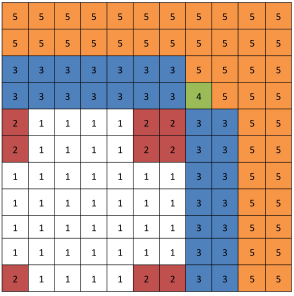
\includegraphics[width=0.4\linewidth]{core}
  \caption{Core Geometry}
  \label{geom}
\end{figure}
\subsection{Mathematical Model}
The PDE describing steady-state neutron transport in the core is the two-group neutron diffusion criticality approximation,
\begin{equation}
-\grad\cdot\qty( D_1(\bar x)\grad\phi_1(\bar x))+\qty(\xs{a}{1}(\bar x)+\xs{s}{1\to2}(\bar x))\phi_1(\bar x) = \frac{1}{k(\phi)}\sum_{g'=1}^2\nu_{g'}\xs{f}{g'}(\bar x)\phi_{g'}(\bar x),
\end{equation}
\begin{equation}
-\grad \cdot\qty(D_2(\bar x)\grad \phi_2(\bar x))+\xs{a}{2}(\bar x)\phi_2(\bar x) = \xs{s}{1\to 2}(\bar x)\phi_1(\bar x),
\end{equation}
where we use the following parametric coefficients: the absorption cross section $\Sigma_{g,a}=\Sigma_{g,c}+\Sigma_{g,f}$; the capture and fission cross sections $\Sigma_{g,c}$ and $\Sigma_{g,f}$; the diffusion coefficient $D_g$ which depends on the scattering cross section of the medium; and the fission multiplication factor $\nu_g$, the ratio of new neutrons per fission-producing neutron.  The solution to this PDE is the neutron scalar flux $\phi_g(\bar x)$.  We apply no-traction conditions on the vacuum boundaries and zero-derivative current on the reflecting boundaries for both energy groups:
 \begin{equation}
\frac{\phi_g}{4}-\frac{D_g}{2}\eval{\pdv{\phi_g}{x_1}}_{\partial \Omega_\text{top}}=0,\hspace{5pt} g=1,2,
\end{equation}
\begin{equation}
\frac{\phi_g}{4}-\frac{D_g}{2}\eval{\pdv{\phi_g}{x_2}}_{\partial \Omega_\text{right}}=0,\hspace{5pt} g=1,2,
\end{equation}
\begin{equation}
-D_g\eval{\pdv{\phi_g}{x_1}}_{\partial \Omega_\text{bottom}}=0,\hspace{5pt} g=1,2,
\end{equation}
\begin{equation}
-D_g\eval{\pdv{\phi_g}{x_2}}_{\partial \Omega_\text{left}}=0,\hspace{5pt} g=1,2.
\end{equation}

The material properties are shown in Table \ref{tab:coremats}, and the domain $\Omega=[0,200\text{ cm}]^2$.  The reference flux solutions are plotted in Fig. \ref{benchflux}, and for the reference problem $k$=1.00007605445.

\begin{table}[h]
\centering
\begin{tabular}{c c | c c c c}
Region & Group & $D_g$ & $\Sigma_{a,g}$ & $\nu\Sigma_{f,g}$ & $\Sigma_s^{1,2}$ \\ \hline
1 & 1 & 1.255 & 8.252e-3 & 4.602e-3 & 2.533e-2 \\
 & 2 & 2.11e-1 & 1.003e-1 & 1.091e-1 & \\ \hline
2 & 1 & 1.268 & 7.181e-3 & 4.609e-3 & 2.767e-2 \\
 & 2 & 1.902e-1 & 7.047e-2 & 8.675e-2 & \\ \hline
3 & 1 & 1.259 & 8.002e-3 & 4.663e-3 & 2.617e-2 \\
 & 2 & 2.091e-1 & 8.344e-2 & 1.021e-1 & \\ \hline
4 & 1 & 1.259 & 8.002e-3 & 4.663e-3 & 2.617e-2 \\
 & 2 & 2.091e-1 & 7.3324e-2 & 1.021e-1 & \\ \hline
5 & 1 & 1.257 & 6.034e-4 & 0 & 4.754e-2 \\
 & 2 & 1.592e-1 & 1.911e-2 & 0 & 
\end{tabular}
\caption{Reference Material Properties for Benchmark Core}
\label{tab:coremats}
\end{table}
\begin{figure}[h]
\centering
  \begin{subfigure}[b]{0.45 \textwidth}
   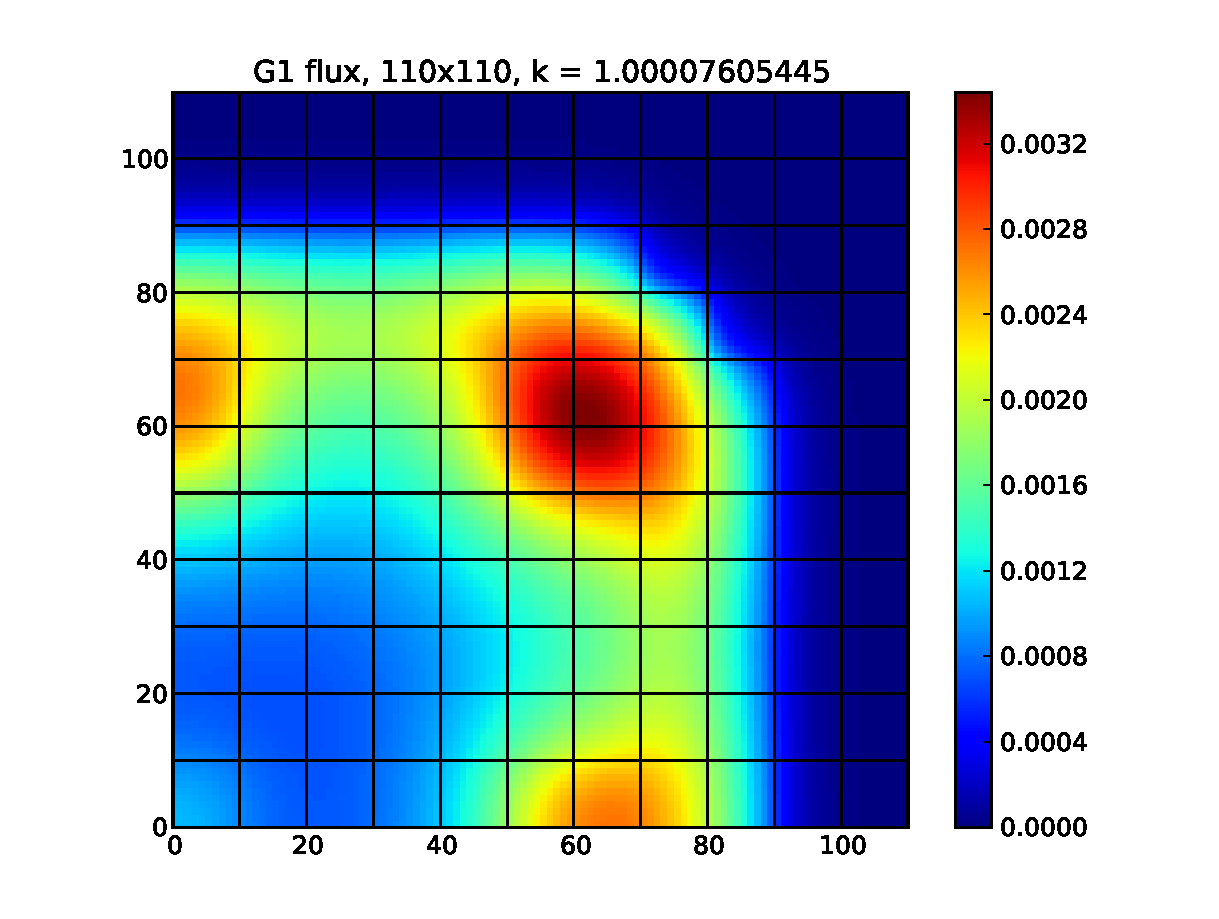
\includegraphics[width=\textwidth]{g1_50_flux}
   \caption{$\phi$, Group 1}
   \label{g1}
  \end{subfigure}
  \begin{subfigure}[b]{0.45 \textwidth}
   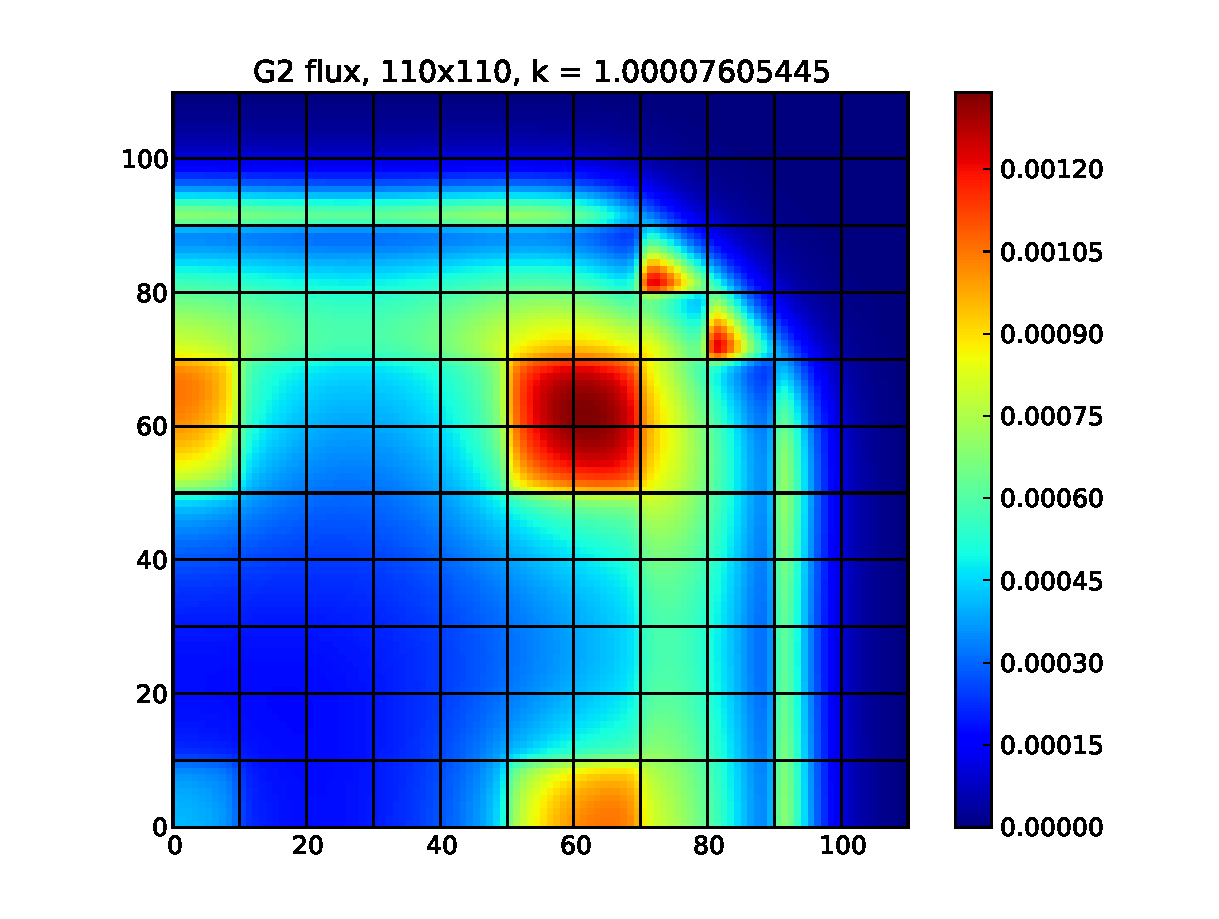
\includegraphics[width=\textwidth]{g2_50_flux}
   \caption{$\phi$, Group 2}
   \label{g2}
  \end{subfigure}
  \caption{Reference Flux Profiles}
  \label{benchflux}
\end{figure}

\subsection{Deterministic Solver}
The criticality eigenvalue and quantity of interest $k(\phi)$ is converged on iteratively by
\begin{equation}
k^{n+1}=k^n\sum_{g=1}^2\frac{\iint\limits_\Omega\nu\xs{f}{g}\phi_g^{n+1}(\bar x)~d\bar x}{\iint\limits_\Omega\nu\xs{f}{g}\phi_g^{n}(\bar x)~d\bar x}.
\end{equation}
until a convergence tolerance is achieved.  We solve $\phi_1,\phi_2,$ and $k$ nonlinearly and simultaneously using a globally- and locally-conservative finite volume approximation in space.  We solve implicitly with a Jacobian-Free Newton Krylov method, using a GMRES package from nonlinear solver package \texttt{trilinos} \cite{Trilinos-Overview}.

To verify the deterministic solver, we compare flux profiles and $k$ to the original benchmark\cite{benchmark} as well as demonstrate the convergence of $k$ with increasing mesh grid refinement.  The deterministic solver is in agreement with the benchmark, and convergence for $k$ and both group fluxes are demonstrated in Fig. \ref{det-conv}.  Both fluxes as well as the $k$-eigenvalue converge between first and second order.  The finite volume method is second order, but the overall convergence order is reduced by first-order boundary condition treatments.  In all cases, reducing the size of $h=\Delta x=\Delta y$ decreases the error in the solution.  The reference solution is a level of refinement finer than the finest point shown.   The flux error is calculated by considering the maximum error among several point-wise flux values, while $k$ error is the global value for each refinement.
\begin{figure}[h]
\centering
  \begin{subfigure}[b]{0.3 \textwidth}
   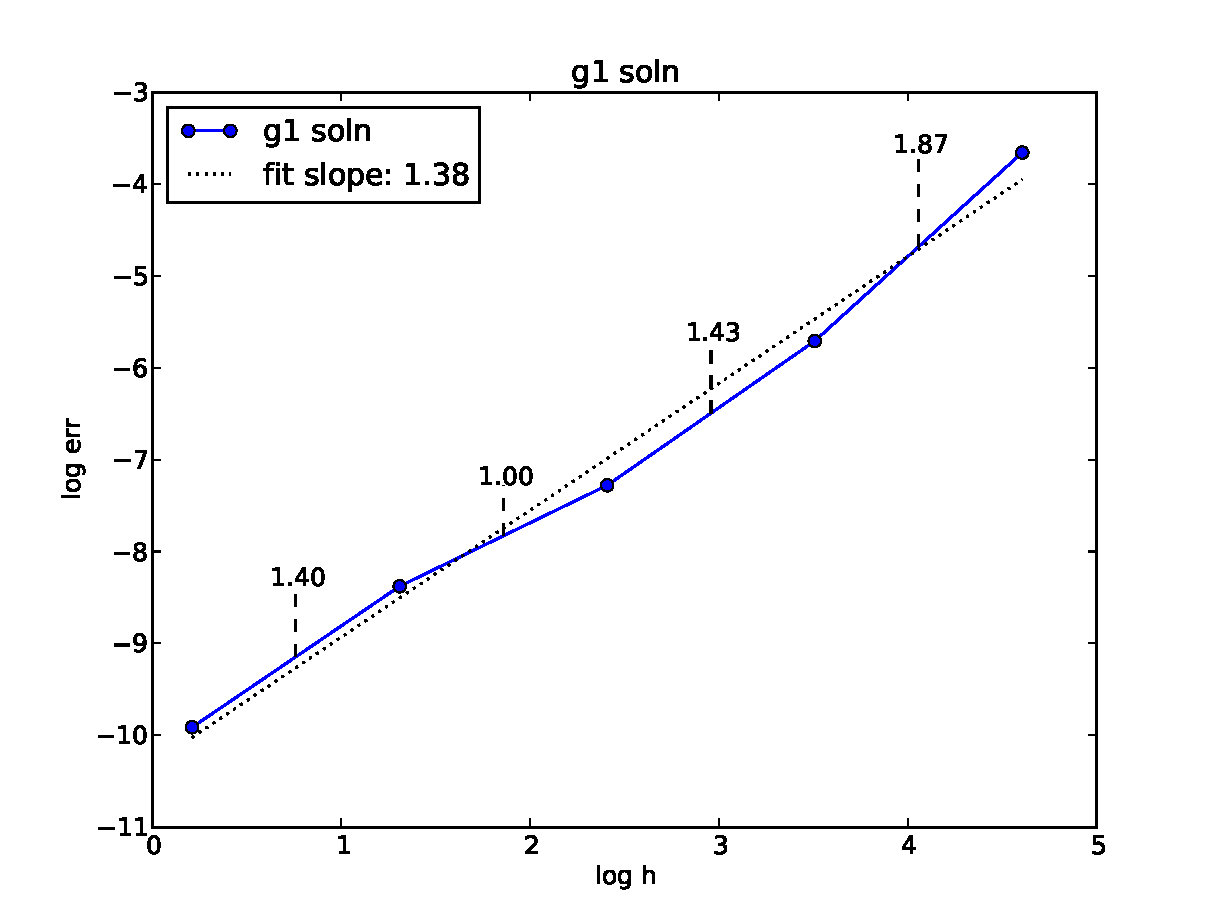
\includegraphics[width=\textwidth]{g1}
   \caption{$\phi$, Group 1}
   \label{g1conv}
  \end{subfigure}
  \begin{subfigure}[b]{0.3 \textwidth}
   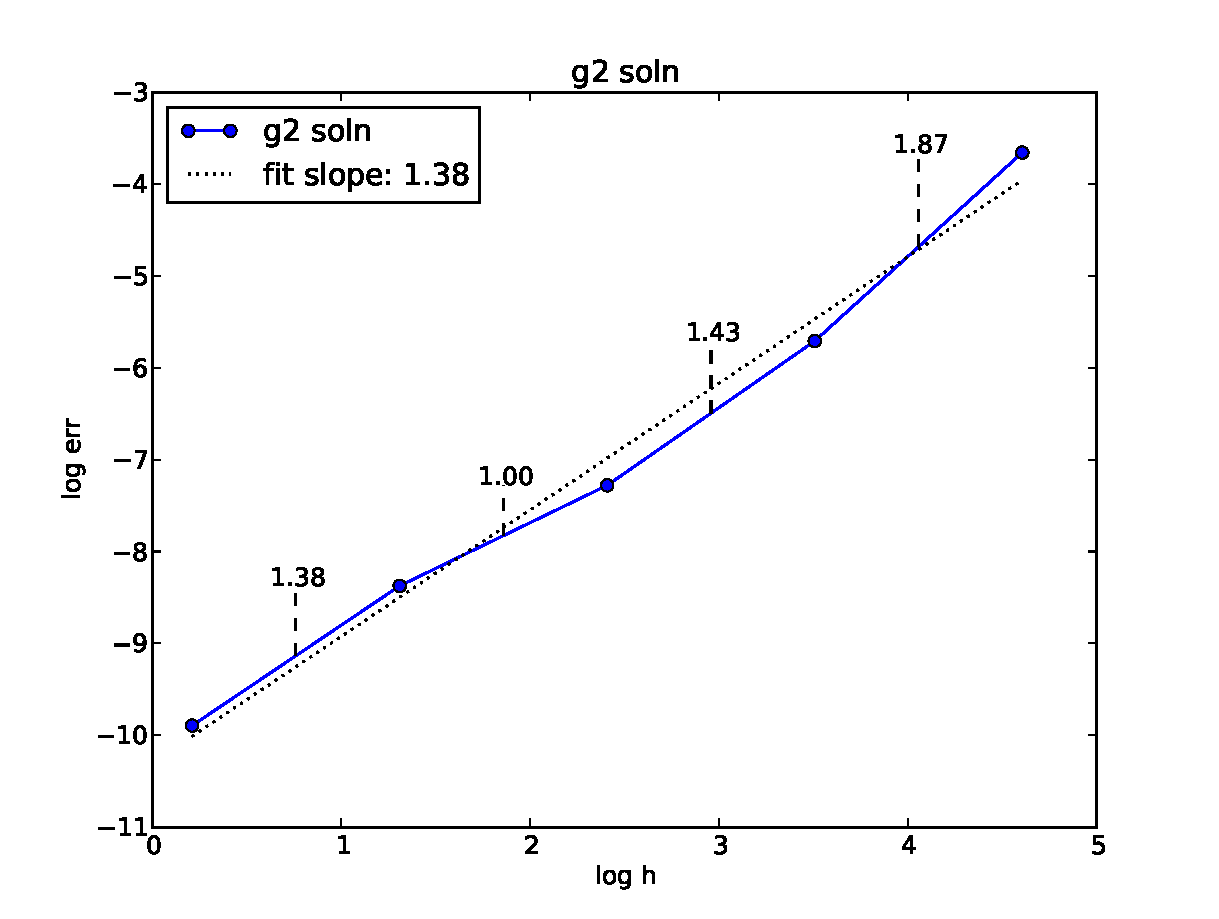
\includegraphics[width=\textwidth]{g2}
   \caption{$\phi$, Group 2}
   \label{g2conv}
  \end{subfigure}
  \begin{subfigure}[b]{0.3 \textwidth}
   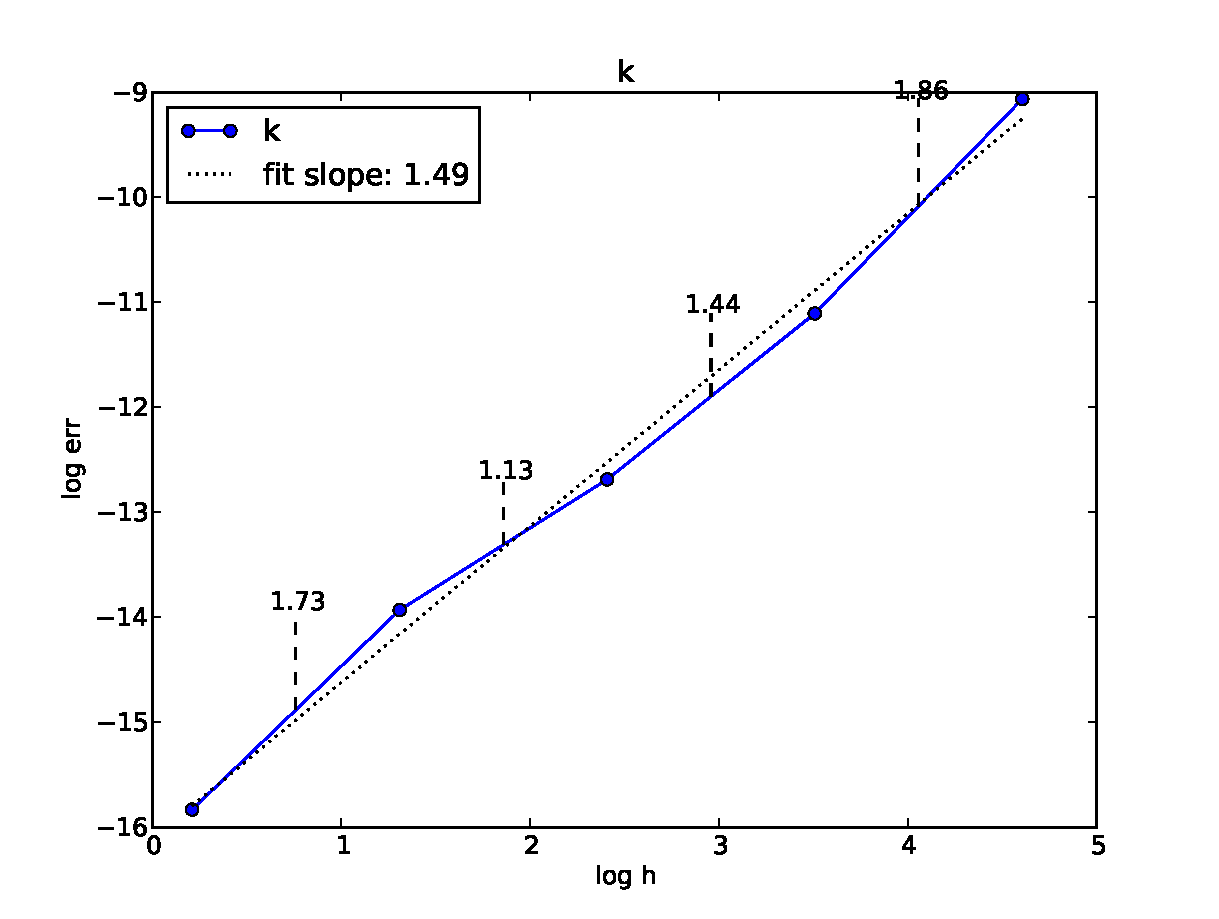
\includegraphics[width=\textwidth]{k}
   \caption{$k$}
   \label{kconv}
  \end{subfigure}
  \caption{Deterministic Solver Convergence}
  \label{det-conv}
\end{figure}

%%%%%%%%%%%%%%%%%%%%%%%%%%%%%%
%%%%%%%%%%%%%%%%%%%%%%%%%%%%%%
%%%%%%%%%%%%%%%%%%%%%%%%%%%%%%

\section{Uncertainty Quantification}
Throughout the remainder of this document, we will represent the solution to the $k$-eigenvalue problem generically as $u(Y)$, where $u$ corresponds to the value of $k$ and $Y$ is the vector of uncertain input parameters.

There are 33 total input parameters in Table \ref{tab:coremats} that can be treated as uncertain.  For simplicity, any uncertainty introduced by these parameters is taken to be uniformly distributed within 10\% of the reference value.  We consider three cases for uncertainty quantification, distinguished chiefly by the number of input parameters with uncertainty ($N$): material 1 uncertainty, where all the material properties for material 1 are treated as uncertain ($N$=7); low-energy group uncertainty, where all material properties for group 2 are treated as uncertain ($N$=13); and full uncertainty, where all material properties are treated as uncertain ($N$=33).

The test for a method's effectiveness will be considering the level of error reached as a function of the number of calls to the deterministic solver required.  While there is some difference in overhead cost between methods, this diminishes for sufficiently costly deterministic solutions.

In general, moments of the quantity of interest $u(Y)$ are obtained by
\begin{equation}
\expv{u(Y)^r} = \int_\Gamma u(Y)^r P(Y) dY,
\end{equation}
where $r$ is the desired moment, $Y=[Y_1,Y_2,\ldots,Y_N]$ are the uncertain inputs, $P(Y)$ is the joint probability distribution of $Y$, and $\Gamma$ is the uncertainty space spanned by $Y$.

\subsection{Monte Carlo}
By way of benchmark, we consider analog Monte Carlo (MC) as a benchmark uncertainty quantification technique.
Analog Monte Carlo determines the moments of a function by randomly sampling from the uncertainty space repeatedly until an accurate idea of the result is obtained.  Monte Carlo benefits from a guaranteed consistent rate of convergence; however, this convergence rate is quite low; it typically converges as 1 over the square root of the number of deterministic solves.
MC approximates moments of $u(Y)$ as
\begin{equation}
\expv{u(Y)^r}\approx \frac{1}{\eta}\sum_{m=1}^\eta u(Y^{(m)})^r,
\end{equation}
where $\eta$ is the total number of samples taken, $m$ is the index of a sample, and $Y^{(m)}$ is a point randomly sampled from $\Gamma$.


\subsection{Stochastic Collocation}
In stochastic collocation, we approximate $u(Y)$ as the sum of $u$ evaluated at $\eta$ collocated points multiplied by multidimensional Lagrangian polynomials.  We make use of the quadrature index $k$, not to be confused with the criticality factor $k(Y)$ (represented by $u(Y)$).
\begin{equation}\label{approx}
u(Y)\approx u_{h,\eta,\Lambda(L)}(Y)=\sum_{k=0}^\eta u(Y^{(k)})\mathcal{L}_k(Y),
\end{equation}
\begin{equation}
\mathcal{L}_k(Y)=\prod_{n=1}^N \mathcal{L}_{k_n}(Y_n),
\end{equation}
\begin{equation}
\mathcal{L}_{k_n}(Y_n)=\prod_{j=1}^i \frac{Y_n-Y_n^{(i)}}{Y_n^{(k_n)}-Y_n^{(i)}},
\end{equation}
\begin{equation}
\expv{u(Y)}\approx\expv{u_h(Y)}=\sum_{k=1}^\eta w_k ~u_h\qty(Y^{(k)}),
\end{equation}
where $u_h(Y)$ is the spatially-discretized PDE solution, and $Y^{(k)}=[Y^{(k_1)},\cdots,Y^{(k_N)}]$ are realizations of $Y$ similar to $Y_m$ in Monte Carlo but chosen at quadrature points $Y^{(k)}$ with corresponding weights $w_k$.  For this study, uniformly-distributed uncertain parameters suggest Gauss-Legendre quadrature to obtain collocation points and weights.  The necessary quadrature points are obtained based on polynomial expansion orders from an index set $\Lambda(L)$.

\subsubsection{Index Set $\Lambda(L)$}
The index set $\Lambda(L)$ provides the basis for most of the polynomial representation, including determining the quadrature set to evaluate the sum in Eq. \ref{approx}.  $L$ is the polynomial degree of the stochastic collocation expansion.  For example, for a single uncertain parameter ($N=1$) and a fourth-order polynomial approximation ($L=4$), $\Lambda$ includes all polynomial orders from 0 to 4, $\qty(\Lambda=[0,1,2,3,4])$.  Each index point $p\in\Lambda$ corresponds to a polynomial expansion moment of order $i$.

In the multivariate case, there are several methods to determine what index set to use.
In the most naive case, $\Lambda(L)$ is a tensor product of polynomial expansion orders,
\begin{equation}
\Lambda_\text{TP}(L)=\Big\{\bar p=[p_1,...,p_N]: \max_{1\leq n\leq N}p_n\leq L \Big\},\hspace{10pt}|\Lambda_\text{TP}(L)|=(L+1)^2.
\end{equation}
For example, for $N=2$ and $L=4$, the index set $\Lambda_\text{TP}(L)$ includes all combinations of the expansion orders $[0,1,2,3,4]\otimes[0,1,2,3,4]$ for a total of 25 polynomial expansion indices.  The collection of expansion points in this example index set is shown in Fig. \ref{TP}.  

Other index sets with less cardinality can be employed to reduce the number of collocation points.  Two in particular are the ``total degree'' set (see Fig. \ref{TD}), which is ideal for quantities that are analytic in stochastic space,
\begin{equation}
\Lambda_\text{TD}(L)=\Big\{\bar p=[p_1,...,p_N]:\sum_{n=1}^N p_n \leq L \Big\},\hspace{10pt}|\Lambda_\text{TD}(L)|={L+N\choose N},
\end{equation}
and the ``hyperbolic cross'' index set (see Fig. \ref{HC}), for quantities that have limited smoothness in stochastic space,
\begin{equation}
\Lambda_\text{HC}(L)=\Big\{\bar p=[p_1,...,p_N]:\prod_{n=1}^N p_n+1 \leq L+1 \Big\},\hspace{10pt}|\Lambda_\text{HC}(L)|\leq (L+1)(1+\log(L+1))^{N-1}.
\end{equation}
Figure \ref{indexsets} shows each of these index sets for $N=2,L=4$.  The savings of total degree and hyperbolic cross help fight the curse of dimensionality present in tensor product. 
\begin{figure}[h]
\centering
  \begin{subfigure}[b]{0.32 \textwidth}
   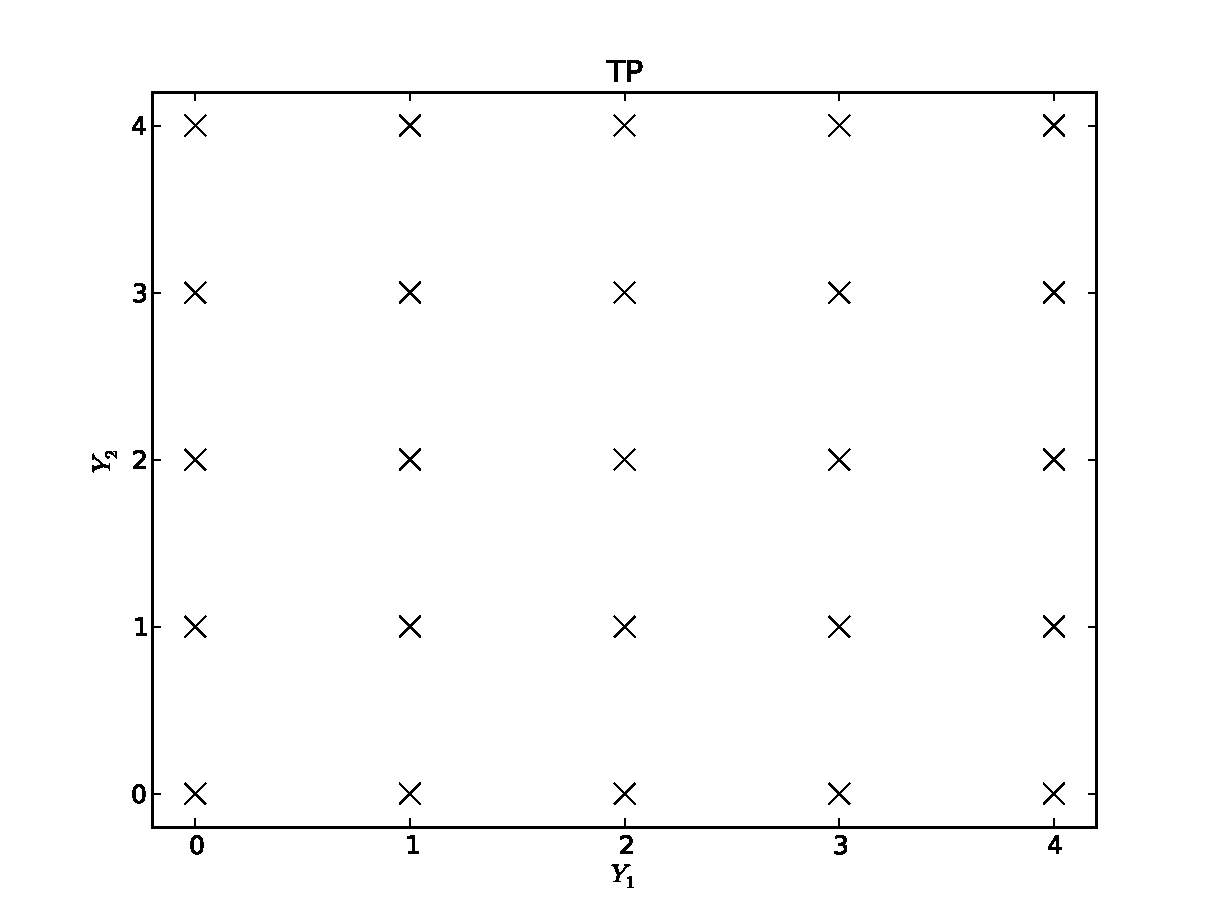
\includegraphics[width=\textwidth]{TP}
   \caption{Tensor Product}
   \label{TP}
  \end{subfigure}
  \begin{subfigure}[b]{0.32 \textwidth}
   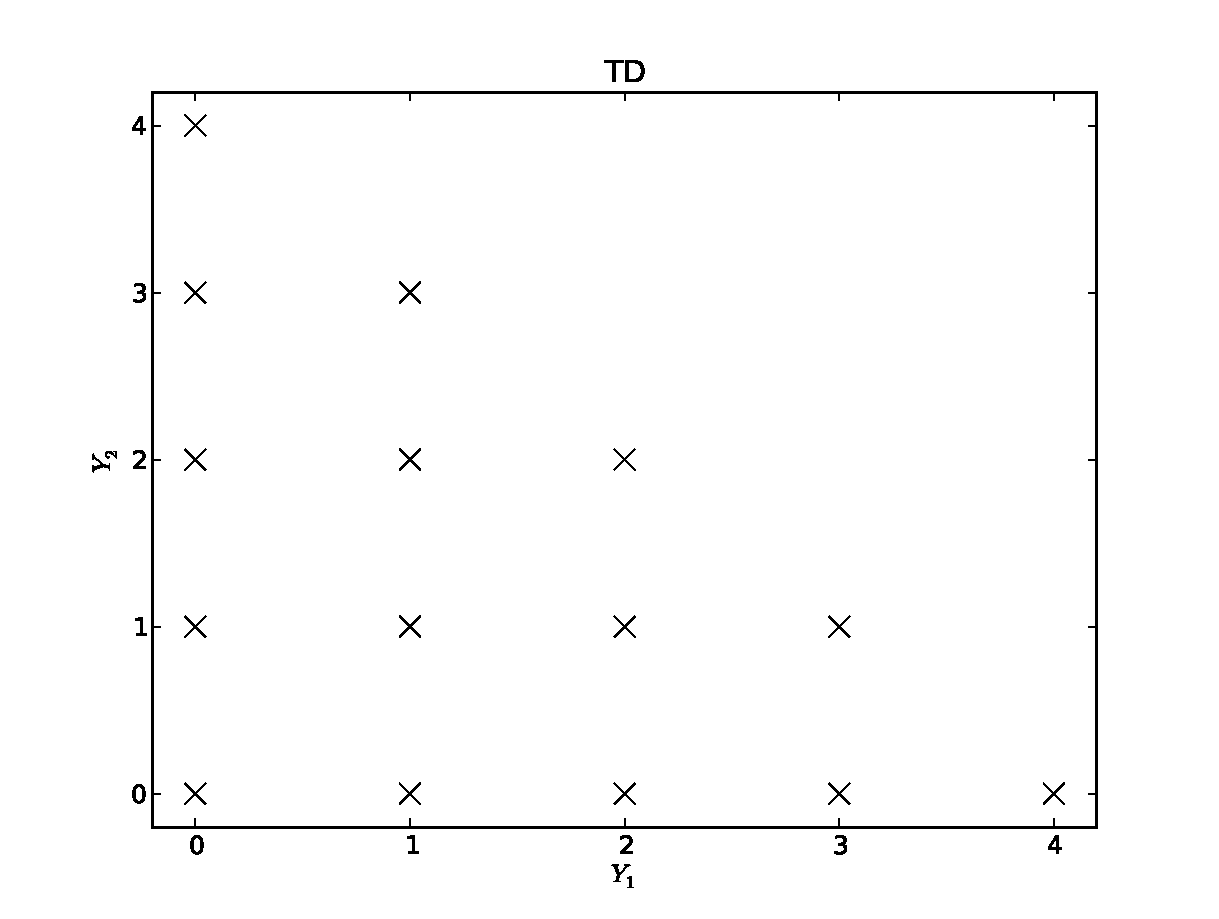
\includegraphics[width=\textwidth]{TD}
   \caption{Total Degree}
   \label{TD}
  \end{subfigure}
  \begin{subfigure}[b]{0.32 \textwidth}
   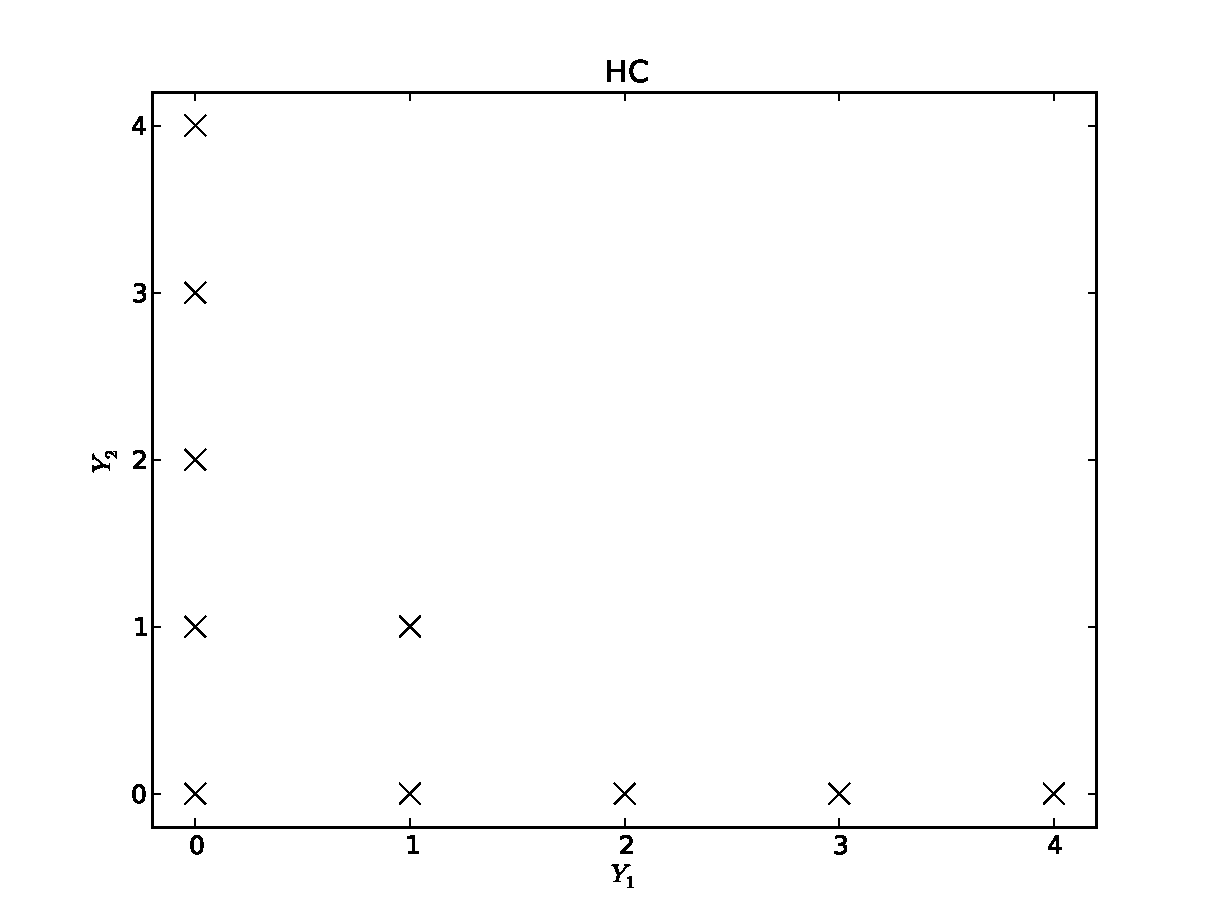
\includegraphics[width=\textwidth]{HC}
   \caption{Hyperbolic Cross}
   \label{HC}
  \end{subfigure}
  \caption{Index Set Examples: $N=2,L=4$}
  \label{indexsets}
\end{figure}

\subsubsection{Sparse Grid Quadrature}
The collocation points used in the Lagrange polynomial expansion are obtained based on the index set chosen.  To uniquely specify an isotropic Smolyak-like sparse grid, it is necessary to determine the number of uncertain variables $N$, the desired expansion order $L$, the index set $\Lambda(L)$, the quadrature rule $p(i)$, and the quadrature points-and-weights generating function for one-dimensional quadratures.
This provides the isotropic sparse grid approximation
\begin{equation}
u(Y)\approx\mathcal{S}_{N,\Lambda(L)}[k](Y)=\sum_{\boldsymbol{i}\in\Lambda(L)}c(\boldsymbol{i})\bigotimes_{n=1}^N\mathcal{U}_{n,p(i_n)}[u](Y),
\end{equation}
\begin{equation}
c(\boldsymbol{i})=\sum_{\substack{\boldsymbol{j}=\{0,1\}^N,\\ \boldsymbol{i}+\boldsymbol{j}\in\Lambda(L)}}(-1)^{|\boldsymbol{j}|_1},
\end{equation}
\begin{align}
\bigotimes_{n=1}^N\mathcal{U}_{n,p(i_n)}[u](Y)&\equiv\sum_{k_1=0}^{p(i_1)}\cdots\sum_{k_N=0}^{p(i_N)}u_h\qty(Y^{(k_1)},\cdots,Y^{(k_N)})\prod_{n=1}^N \mathcal{L}_{k_n}(Y_n),\\
  &=\sum_{k}^{p(\vec i)}u_h\qty(Y^{(k)})\mathcal{L}_k(Y),
\end{align}
where $p(i)$ is the ``quadrature rule'' used to obtain the number of quadrature points for a given expansion order.  While this can be chosen arbitrarily, it is common to select $p(i)=i$ for Gauss quadrature and $p(i)=2^i$ for Clenshaw-Curtis quadrature.
The sparse grid quadrature is obtained through the tensor product of smaller quadratures, which has less cardinality than the full tensor quadrature.  The savings in collocation points are demonstrated in Figure \ref{collsets} for two identically distributed uniform variables, each on [-1,1].  The reduction in collocation points grows with the number of input parameters $N$ and the expansion order $L$.
A visual example of sparse grids for two variables uniformly distributed between -1 and 1 using Gauss-Legendre quadrature is shown in Fig. \ref{collsets}.
\begin{figure}[htb]
\centering
  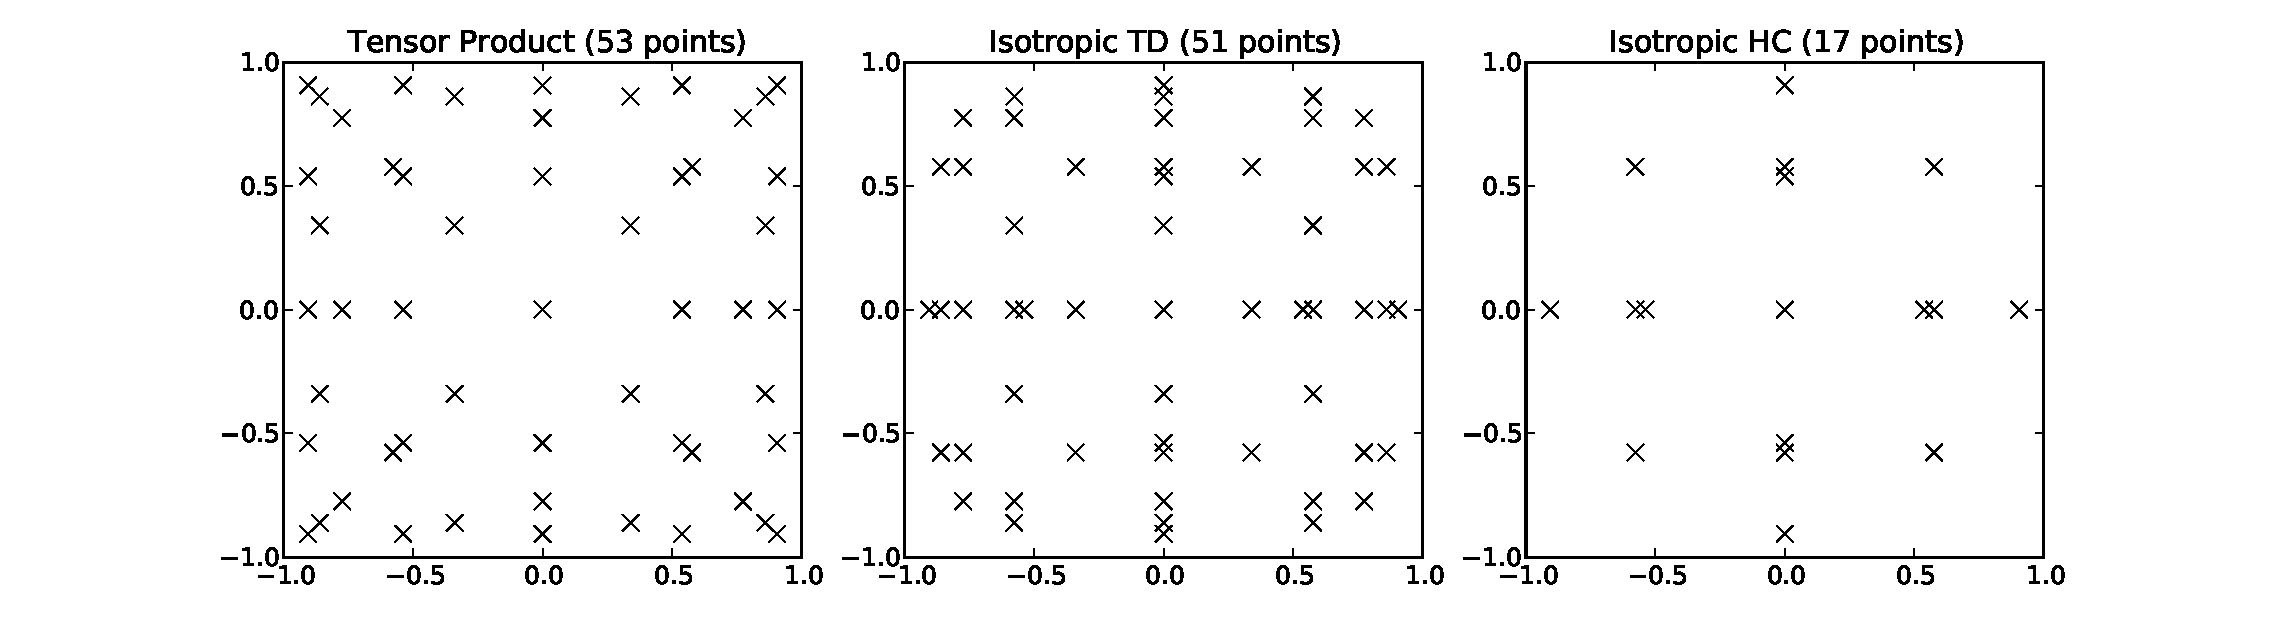
\includegraphics[width=\linewidth]{sparse_plot}
  \caption{Sparse Grids, $N=2,L=4,p(i)=i$, Legendre points}
  \label{collsets}
\end{figure}
For comparison, we show the number of index points for two input spaces of dimensionality $N$ and several expansion levels $L$ for all three index sets, as well as the number of collocation points for total degree and hyperbolic cross rules in Table \ref{compIS}.  We note that accuracy cannot be directly drawn from polynomial expansions; for this problem the same number of collocation points results in a similar magnitude error in both total degree and hyperbolic cross.  This implies, for this problem, that a much lower-order polynomial expansion constructed using the total degree rule is comparable in error to a larger-order polynomial expansion constructed using the hyperbolic cross rule.
\begin{table}[htb]
\centering
\begin{tabular}{c|c|c|c c|c c}
$N$ & $L$ & TP & \multicolumn{2}{|c|}{TD} & \multicolumn{2}{|c}{HC} \\ 
 &  & $\qty|\Lambda(L)|$ & $\qty|\Lambda(L)|$ & $\eta$ & $\qty|\Lambda(L)|$ & $\eta$\\ \hline
3 & 4 & 125    & 35    & 165   & 16 & 31\\
 & 8   & 729    & 165  & 2,097  & 44 & 153\\
 & 16 & 4,913  & 969   & 41,857 & 113 & 513\\ \hline
5 & 2 & 293 & 21 & 61 & 11 & 11\\
 & 4 & 3,125 & 126 & 781 & 31 & 71\\
 & 8 & 59,049 & 1,287 & 28,553 & 111 & 481 
\end{tabular}
\caption{Index Set and Collocation Size Comparison}
\label{compIS}
\end{table}
While the hyberbolic cross collocation points are significantly more sparse than the total degree collocation points, we note that the increased number of polynomial expansion moments in total degree make it much more accurate for the same total polynomial expansion level $L$.  The results of this work demonstrate that for this problem, the same number of collocation points using either total degree or hyperbolic cross results in a similar magnitude of error.

%%%%%%%%%%%%%%%%%%%%%%%%%%%%
%%%%%%%%%%%%%%%%%%%%%%%%%%%%
%%%%%%%%%%%%%%%%%%%%%%%%%%%%

\subsection{Attenuation Problem Results}
Figure \ref{attn} shows the improvement of the various UQ methods discussed as a function of the number of deterministic solves required.  Because each variable contributes identically, anisotropic methods did not show any improvement over collocation.  Given the unlimited smoothness of the uncertainty space, we are not surprised to see the total degree sparse grid for stochastic collocation outperform both Monte Carlo and hyperbolic cross sparse grid.
\begin{figure}[htb]
\centering
  \begin{subfigure}[b]{0.49 \textwidth}
   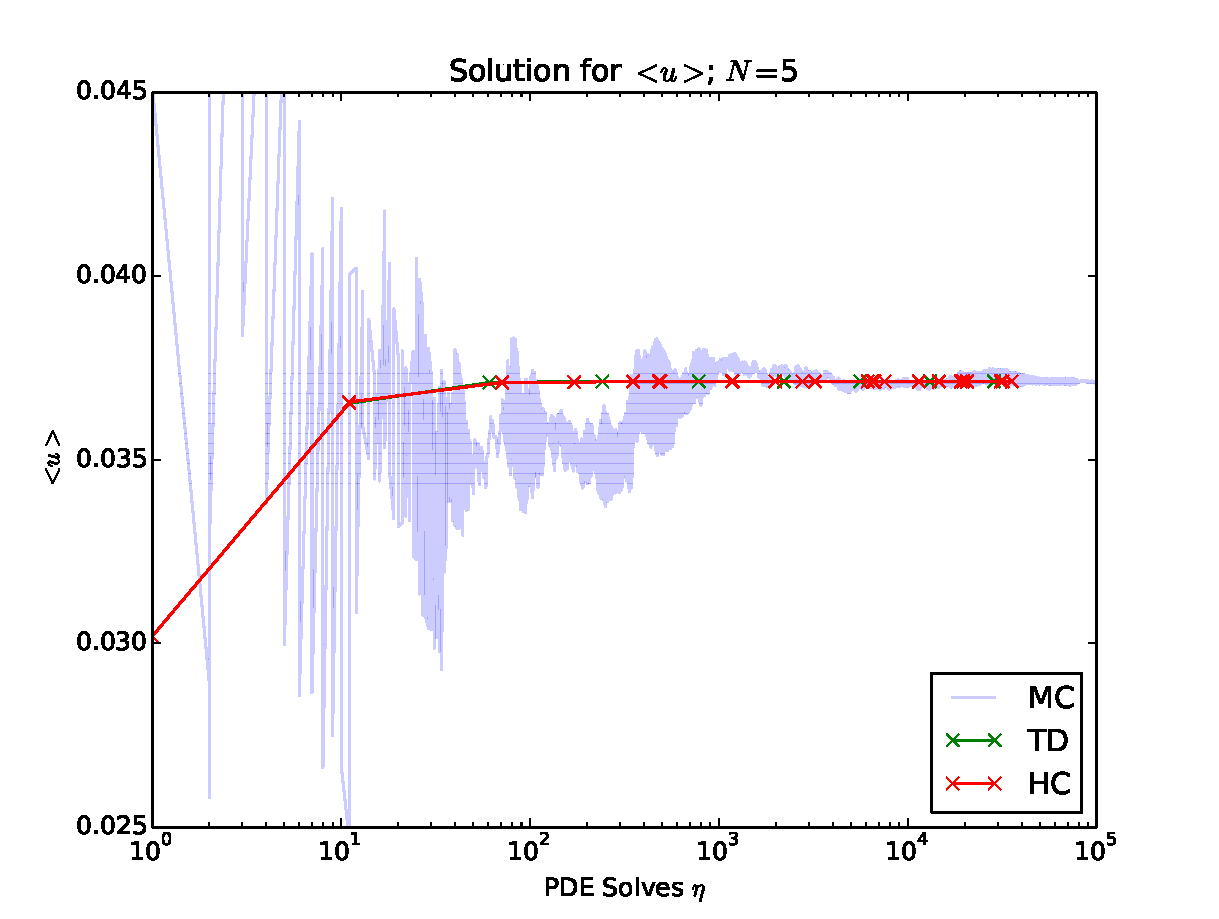
\includegraphics[width=\textwidth]{../graphics/attenuate_N5_soln}
   \caption{Values}
   \label{atn vals}
  \end{subfigure}
  \begin{subfigure}[b]{0.49 \textwidth}
   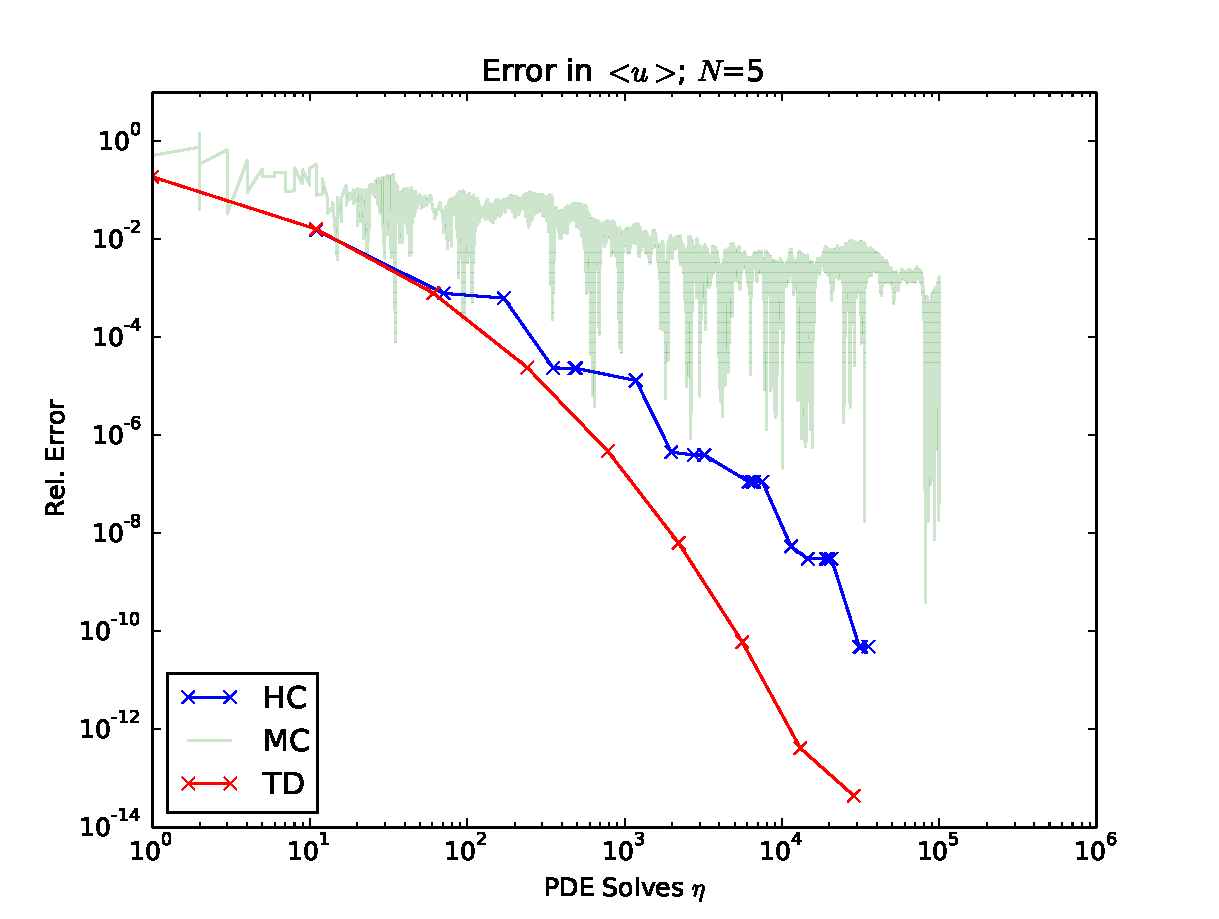
\includegraphics[width=\textwidth]{../graphics/attenuate_N5_conv}
   \caption{Error}
   \label{atn errs}
  \end{subfigure}
  \caption{Attenuation, \expv{u}}
  \label{attn}
\end{figure}
%\begin{figure}[H]
%    \centering
%    %\begin{subfigure}[b]{0.49 \textwidth}
%      \includegraphics[width=0.5\textwidth]{}
%      \caption{$<u>$ Values}
%      \label{atn vals}
%\end{figure}
%\begin{figure}[H]
%\centering
%      \includegraphics[width=0.5\textwidth]{}
%      \caption{Error in $<u>$}
%      \label{atn errs}
%    %\end{subfigure}
%  %\caption{Attenuation UQ Results}
%  %\label{atn results}
%  \end{figure}
\subsection{Projectile Problem Results}
Figure \ref{prj} shows the improvement of the various UQ methods discussed as a function of the number of deterministic solves required.  Because each variable contributes identically, anisotropic methods did not show any improvement over collocation.  The uncertainty space for this problem is significantly less smooth than for the analytic attenuation problem, so we see hyperbolic cross converging more efficiently than total degree.  

There are two particular points of interest in Figure \ref{prj errs}.  First, there is a vertical drop in error at $\eta=11$ solves.  For hyperbolic cross, it is not uncommon for a higher-order polynomial set to require the same number of computational solves as the polynomial order just smaller in order, and yet increase accuracy.  This comes from spending less effort on resolving interactions between uncertainties and more effort on resolving contributions from single inputs.  Second, there is oscillation in the error convergence below an error of about $10^{-5}$.  This is an artifact that arises from the deterministic solver.  Because of the forward-Euler method of the solver, it converges only as well as the time step selected.  In this case, the relative error converged to in the deterministic solver time step was on the order of $10^{-5}$, so the stochastic solver cannot converge the uncertain space any further, and any apparent convergence is incidental.  Tightening the tolerance in the deterministic solver extends the convergence range of the stochastic solver.
\begin{figure}[htb]
\centering
  \begin{subfigure}[b]{0.49 \textwidth}
   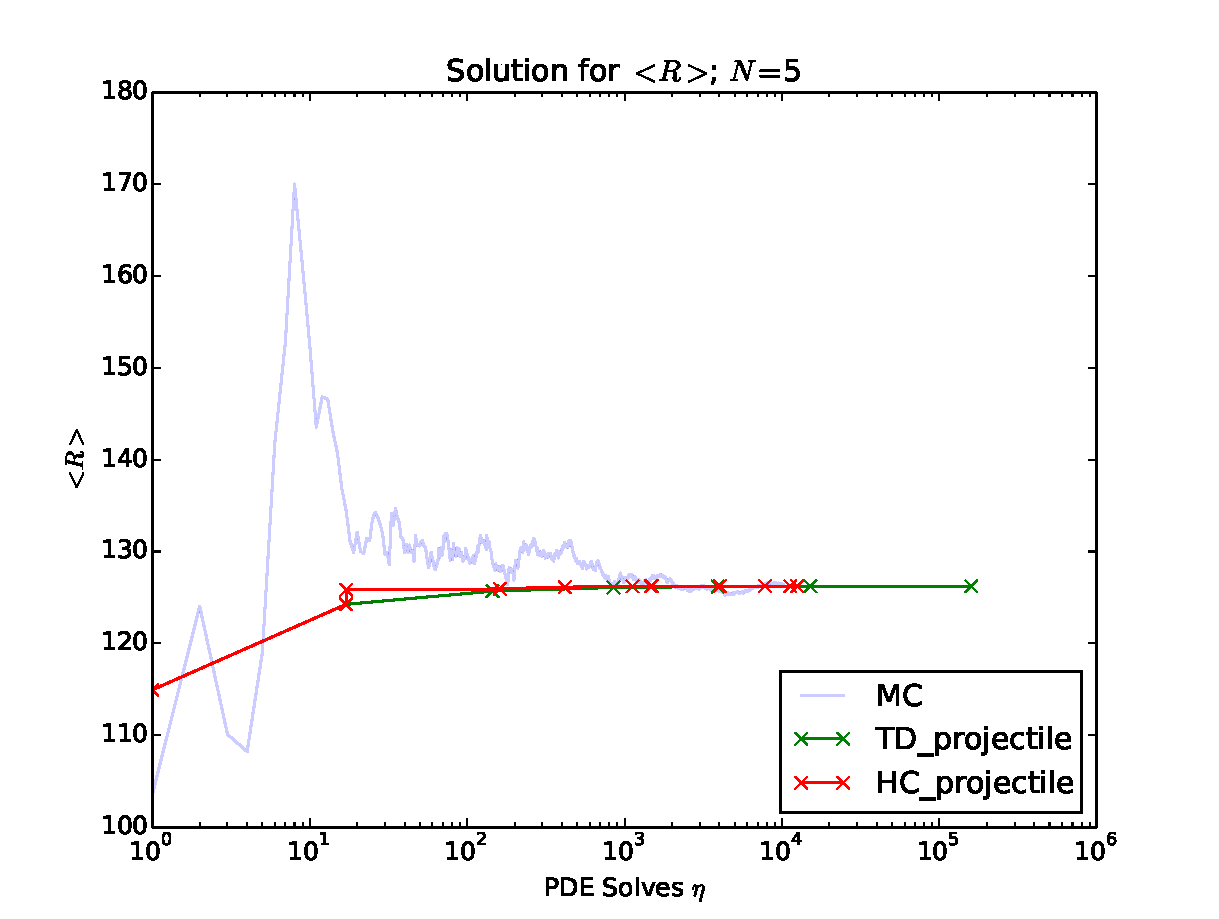
\includegraphics[width=\textwidth]{../graphics/projectile_solns}
   \caption{Values}
   \label{prj vals}
  \end{subfigure}
  \begin{subfigure}[b]{0.49 \textwidth}
   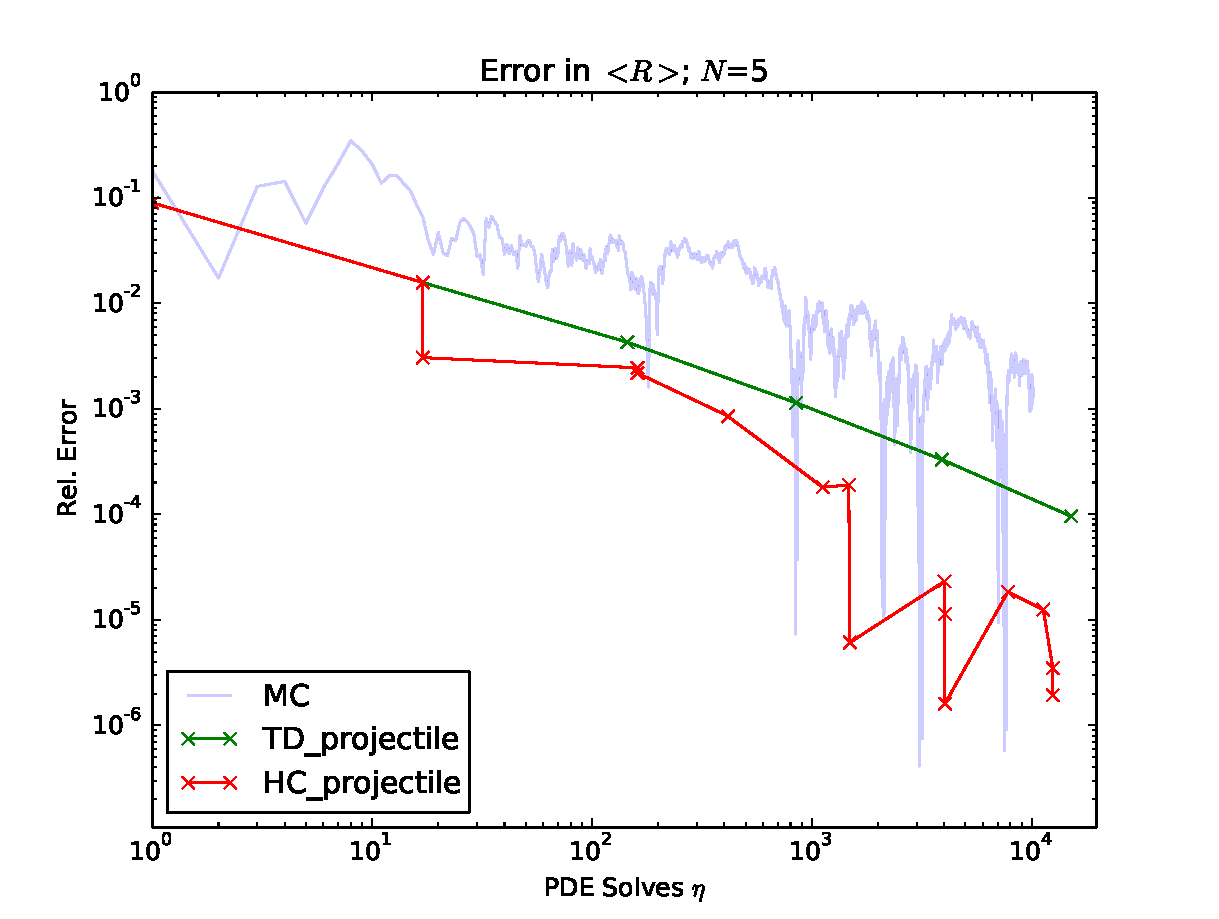
\includegraphics[width=\textwidth]{../graphics/projectile_errs}
   \caption{Error}
   \label{atn errs}
  \end{subfigure}
  \caption{Projectile, \expv{R}}
  \label{prj}
\end{figure}
%\begin{figure}[H]
%    \centering
%    %\begin{subfigure}[b]{0.49 \textwidth}
%      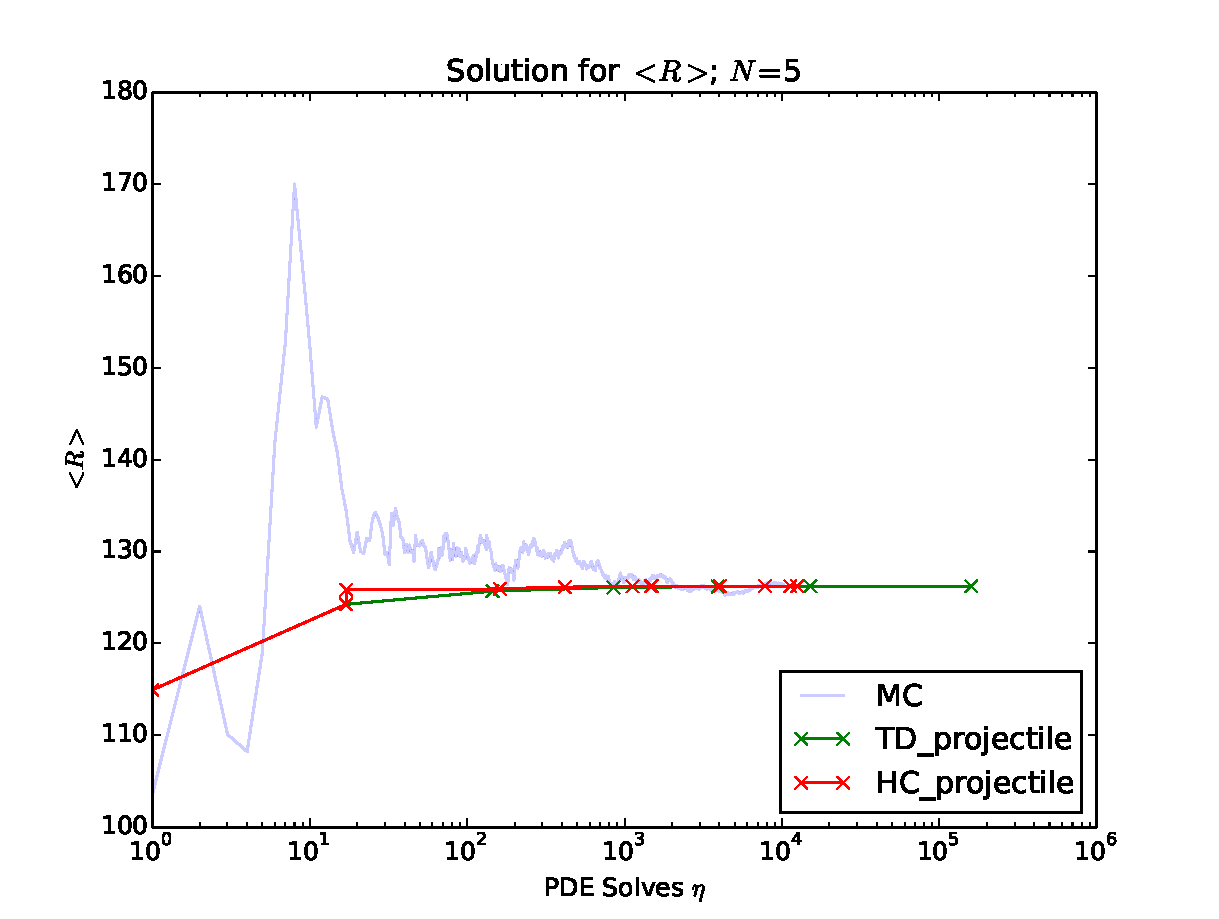
\includegraphics[width=0.5\textwidth]{../graphics/projectile_solns}
%      \caption{$<R>$ Values}
%      \label{prj vals}
%\end{figure}
%\begin{figure}[H]
%\centering
%      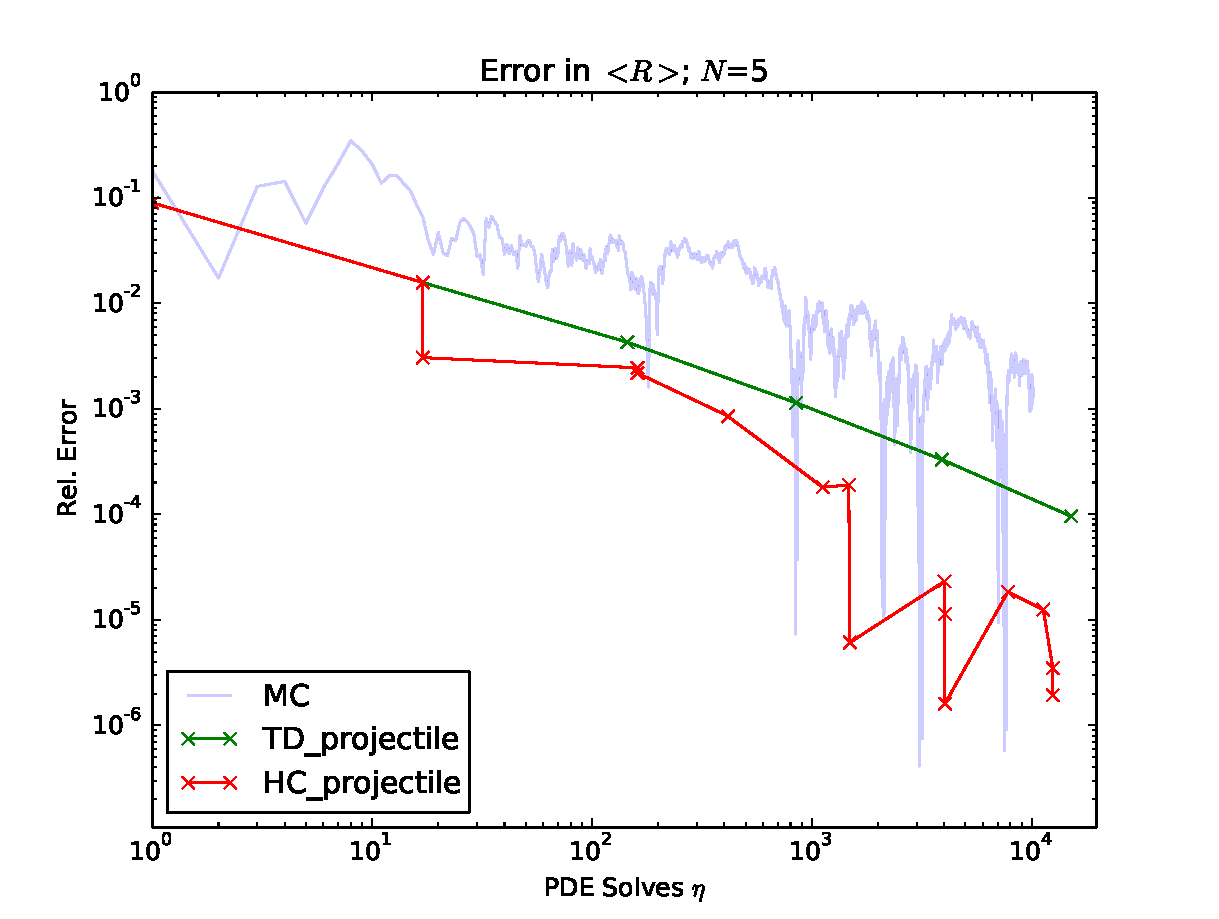
\includegraphics[width=0.5\textwidth]{../graphics/projectile_errs}
%      \caption{Error in $<R>$}
%      \label{prj errs}
%    %\end{subfigure}
%  %\caption{Attenuation UQ Results}
%  %\label{atn results}
%  \end{figure}


\subsection{Diffusion Solver Results}
In order to compare magnitude of error, we use a ``benchmark'' solution generated with a high number of collocation points using isotropic sparse grid stochastic collocation as a reference solution.  Monte Carlo and stochastic collocation solutions for varying numbers of PDE solves are computed, and relative error is plotted as a function of number of solves.  The error is in the moments $r$ of the quantity of interest $k(Y)=u(Y)$, and is given by
\begin{equation}
\epsilon_h^{(r)}=\frac{|\expv{u^{(r)}}-\expv{u_\text{ref}^{(r)}}|}{\expv{u_\text{ref}^{(r)}}},
\end{equation}
\begin{equation}
\expv{u^{(r)}}\approx\expv{S_{N,\Lambda_\text{TD}(L)}[u](Y)^{(r)}}=\sum_{k=1}^\eta w_k ~u^{(r)}\qty(Y^{(k)}),
\end{equation}
where the weights $w_k$ and points $Y^{(k)}$ come from the multivariate quadrature used in stochastic collocation.

Figs. \ref{n1}-\ref{n5} show the comparison of Monte Carlo convergence to stochastic collocation for $N=1,3,5$ where $N$ is the number of uncertain parameters.  Both total degree (TD) and hyperbolic cross (HC) index sets have been included for $N>1$ (they are indistinguishable for $N=1$).  Additionally, we include two low-anisotropy anisotropic grids.

Because of the regularity of $k(Y)=u(Y)$, the total degree index set is as cost effective as the hyperbolic cross index set.  For a less regular stochastic solution, we expect hyperbolic cross would be more efficient.  We also expect the convergence rate to diminish with increasing $N$, and that trend can be seen in the figures for the mean and variance of $k(Y)$. Both the magnitude of the error as well as the convergence rate of stochastic collocation outperforms Monte Carlo for any number of runs.  In addition, heuristic selection of importance weighting improved the accuracy of sparse grid methods by approximately half an order of magnitude.
%\begin{figure}[H]
%\centering
%  \begin{subfigure}[b]{0.49 \textwidth}
%   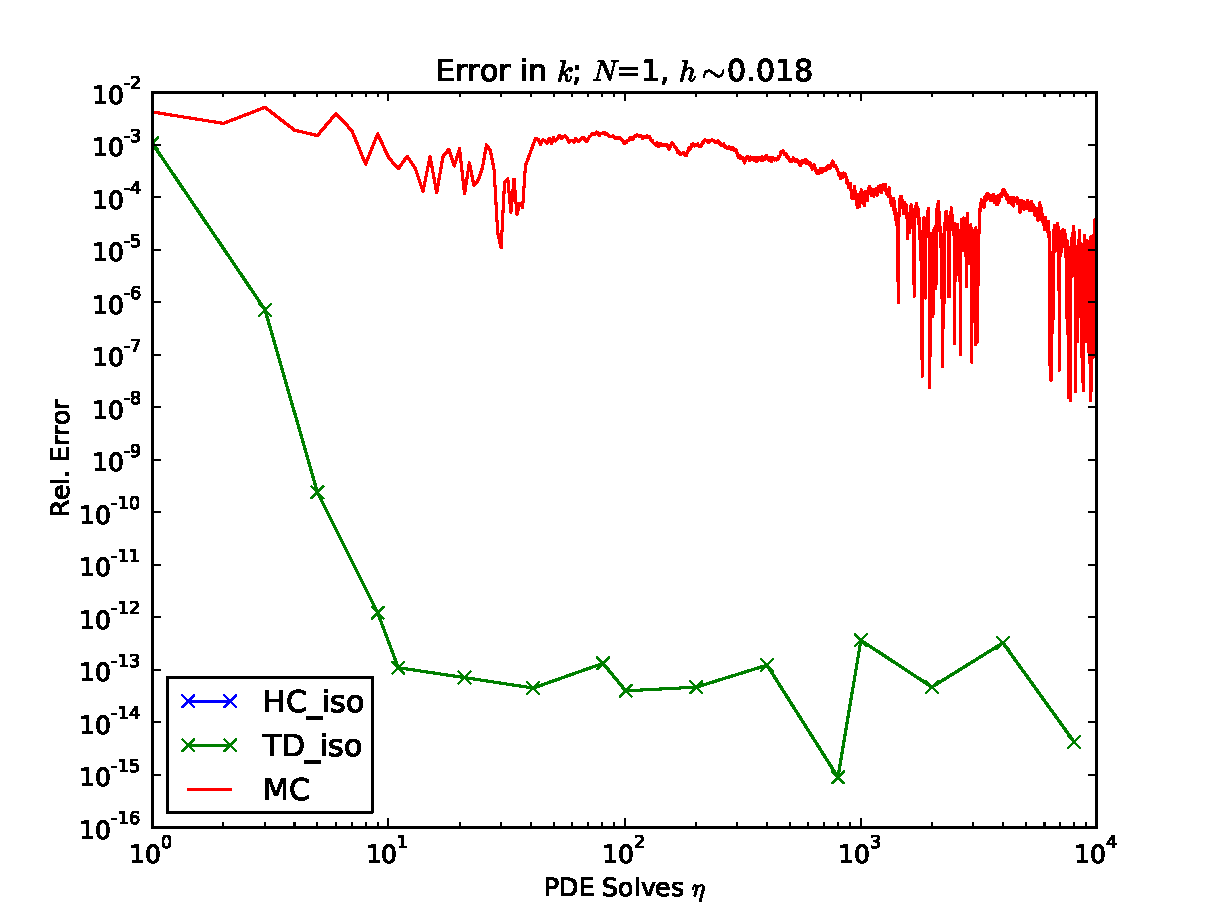
\includegraphics[width=\textwidth]{N1_h5_MCHC}
%   \caption{Mean}
%   \label{n1mean}
%  \end{subfigure}
%  \begin{subfigure}[b]{0.49 \textwidth}
%   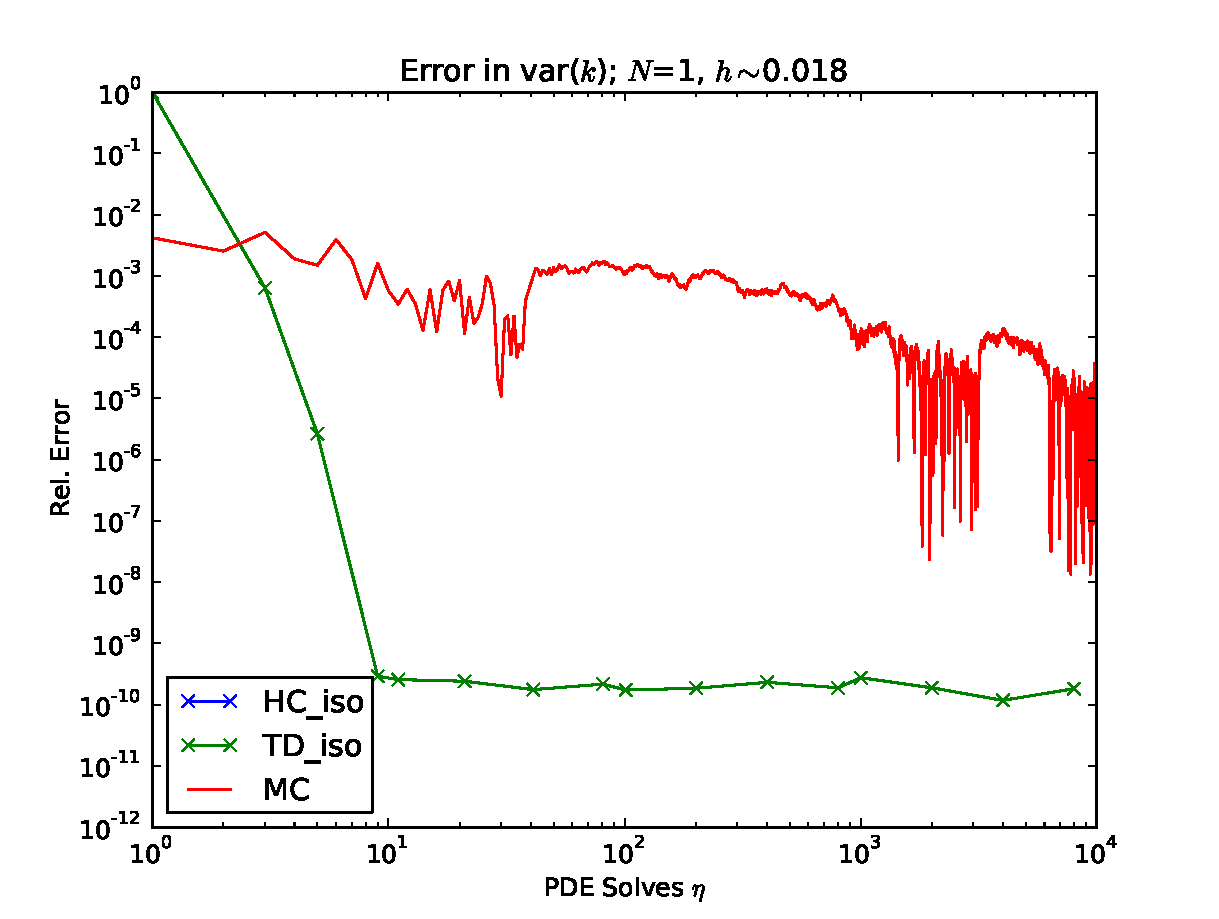
\includegraphics[width=\textwidth]{N1_h5_MCHC_2}
%   \caption{Variance}
%   \label{n1var}
%  \end{subfigure}
%  \caption{$N=1$}
%  \label{n1}
%\end{figure}
%
%\begin{figure}[H]
%\centering
%  \begin{subfigure}[b]{0.49 \textwidth}
%   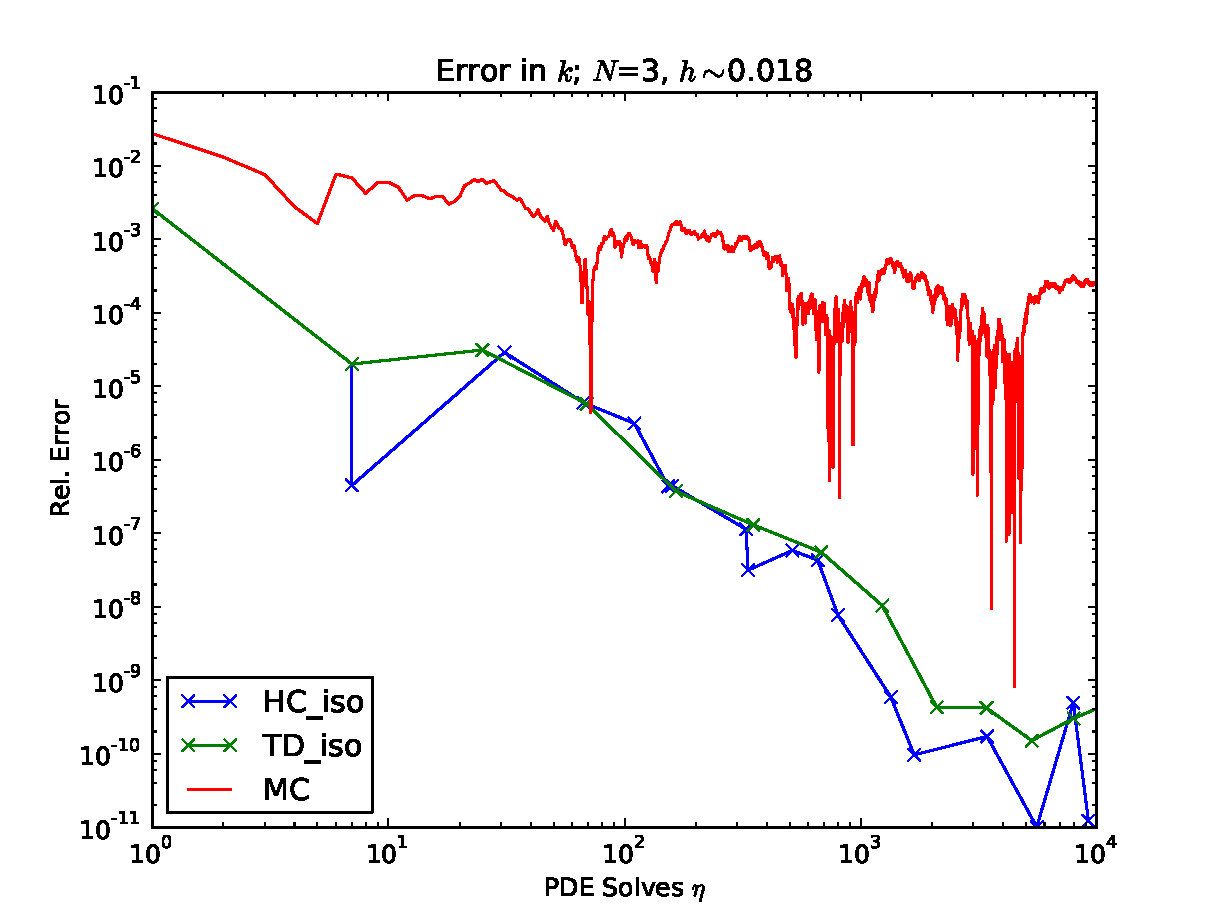
\includegraphics[width=\textwidth]{N3_h5_MCHC}
%   \caption{Mean}
%   \label{n3mean}
%  \end{subfigure}
%  \begin{subfigure}[b]{0.49 \textwidth}
%   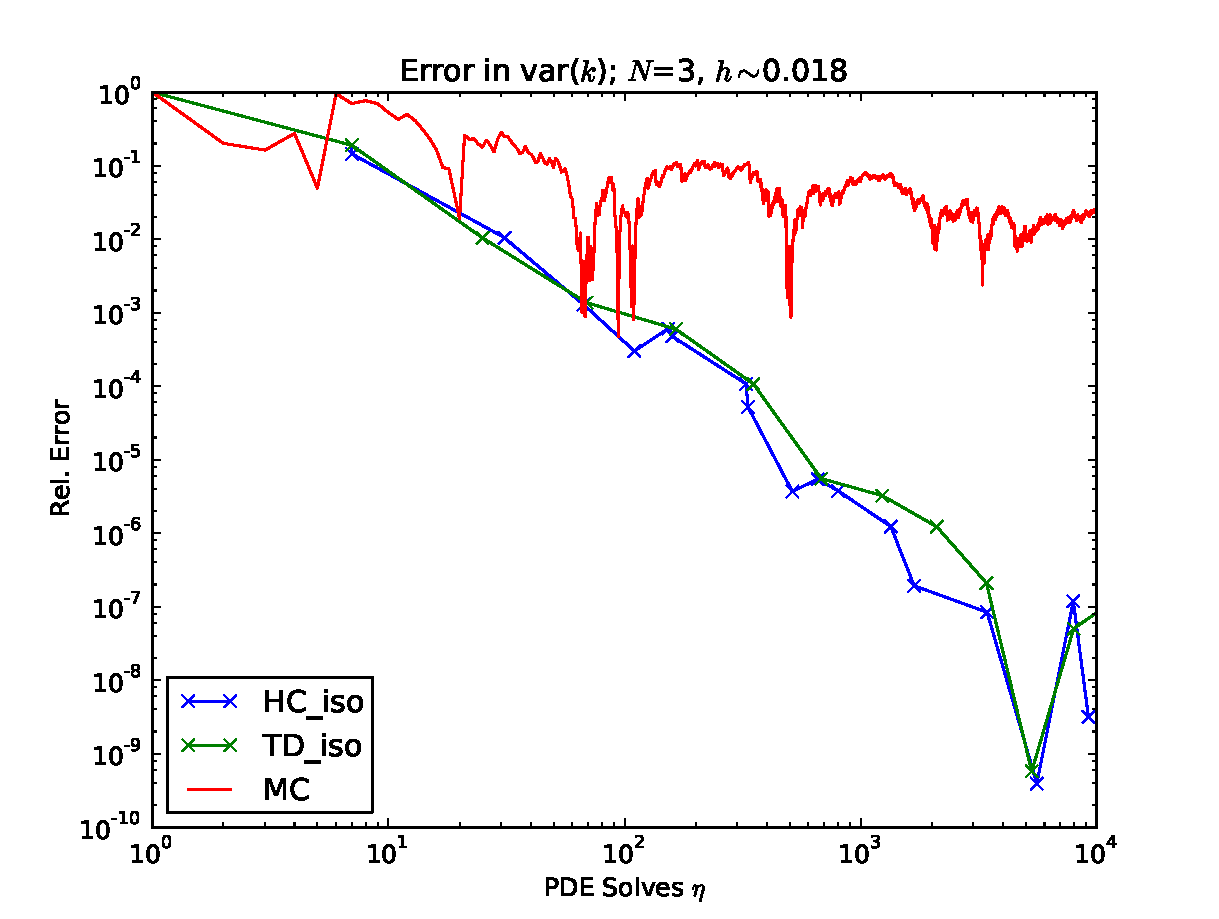
\includegraphics[width=\textwidth]{N3_h5_MCHC_2}
%   \caption{Variance}
%   \label{n3var}
%  \end{subfigure}
%  \caption{$N=3$}
%  \label{n3}
%\end{figure}

\begin{figure}[h]
\centering
  \begin{subfigure}[b]{0.49 \textwidth}
   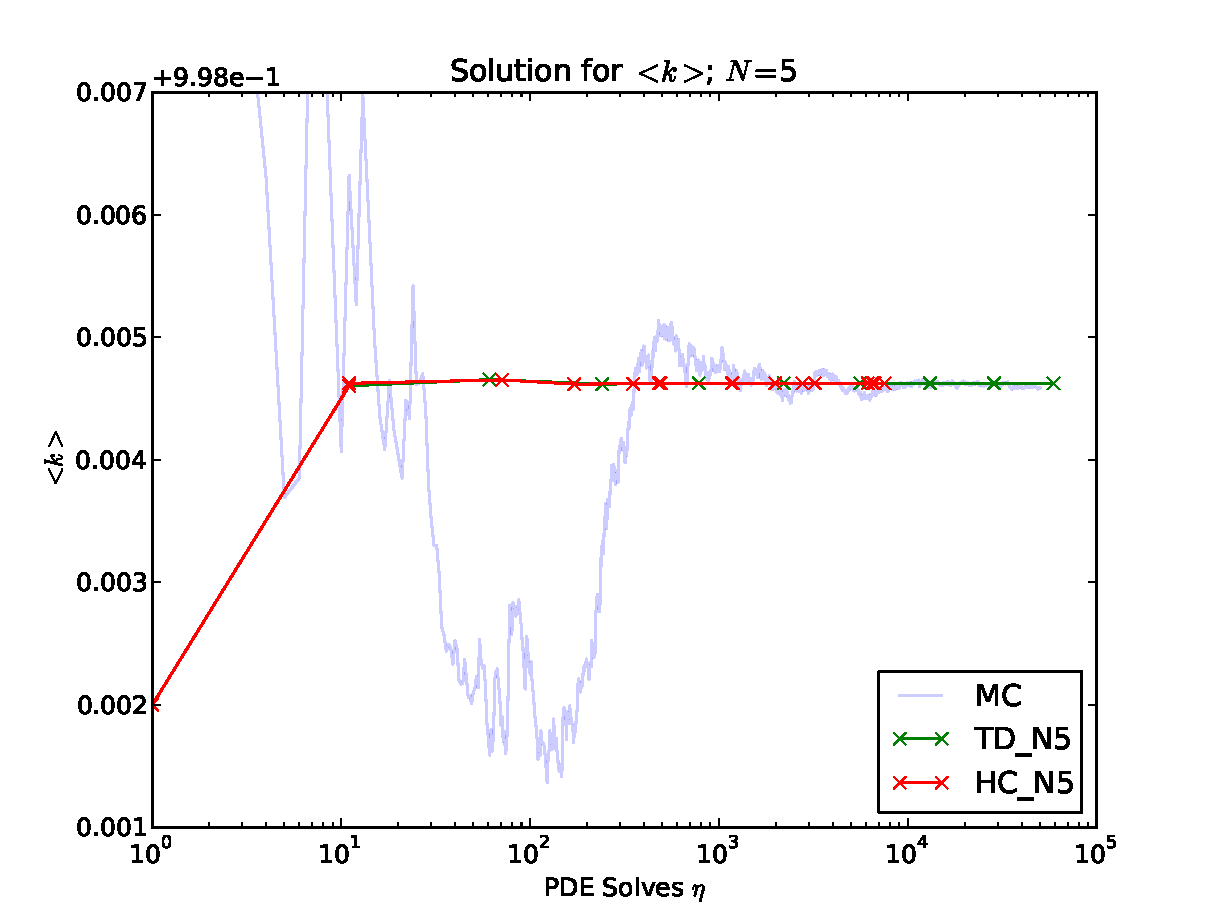
\includegraphics[width=\textwidth]{../graphics/soln_5}
   \caption{Values}
   \label{n5mean}
  \end{subfigure}
  \begin{subfigure}[b]{0.49 \textwidth}
   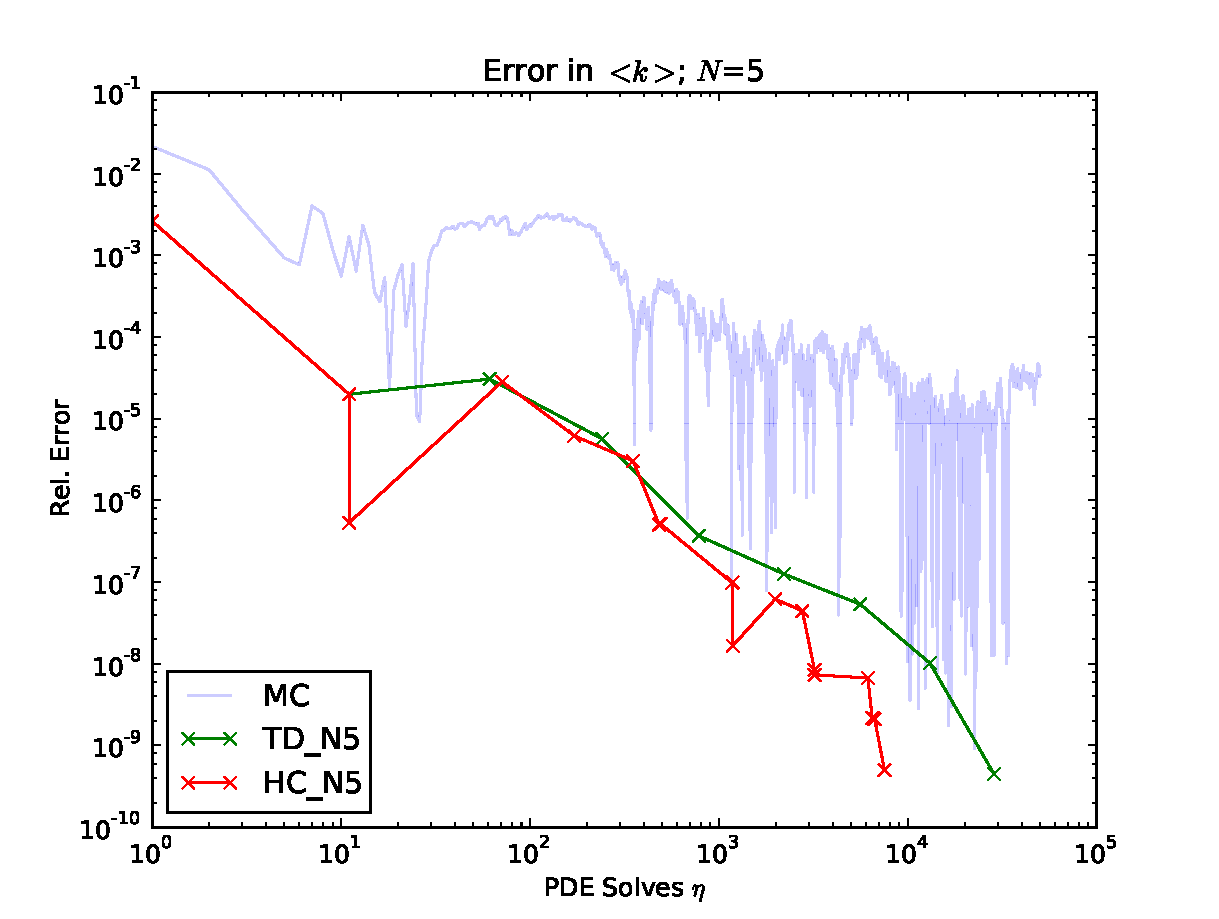
\includegraphics[width=\textwidth]{../graphics/err_5}
   \caption{Errors}
   \label{n5mean}
  \end{subfigure}
  \caption{Diffusion, $N=5$, Mean}
  \label{n5}
\end{figure}

\begin{figure}[h]
\centering
  \begin{subfigure}[b]{0.49 \textwidth}
   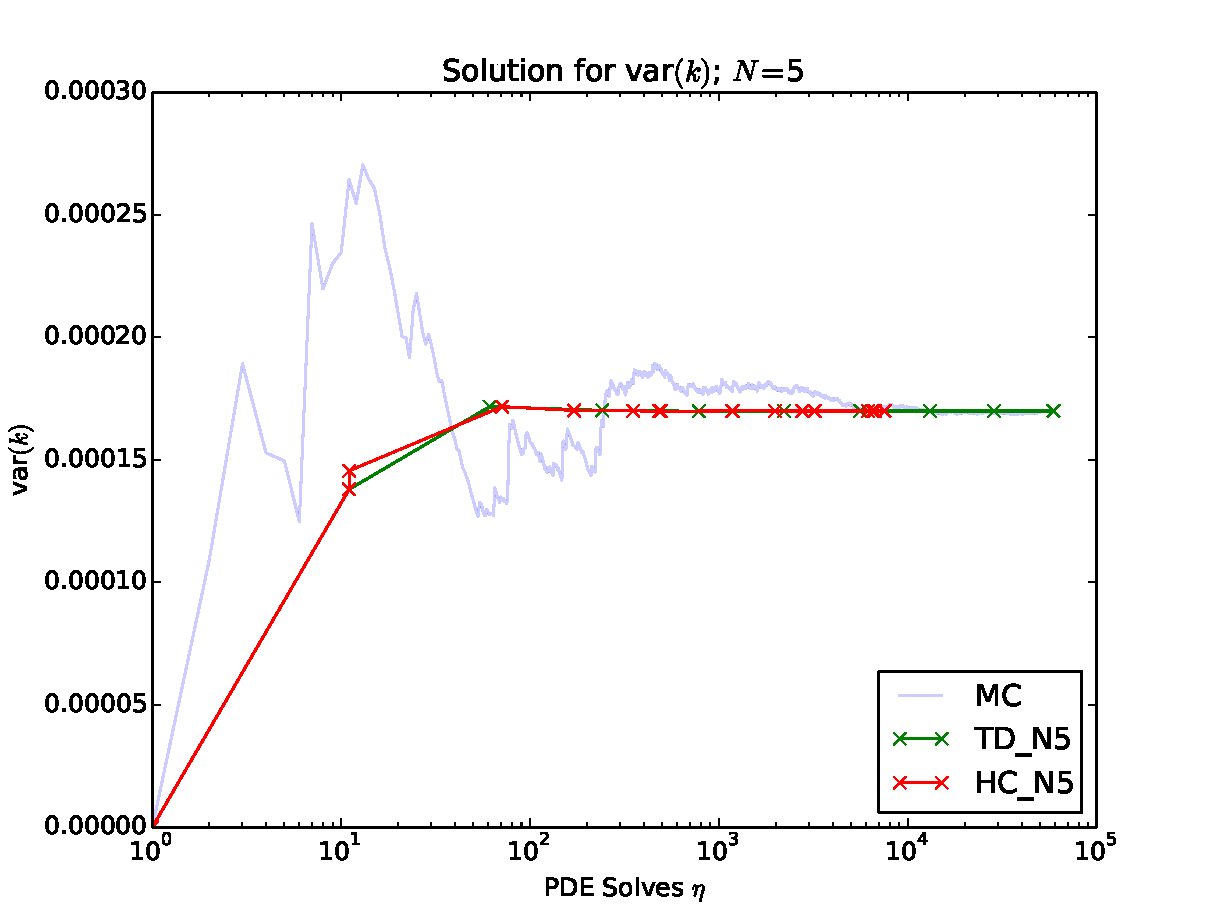
\includegraphics[width=\textwidth]{../graphics/N5_iso_var_vals}
   \caption{Values}
   \label{n5var}
  \end{subfigure}
  \begin{subfigure}[b]{0.49 \textwidth}
   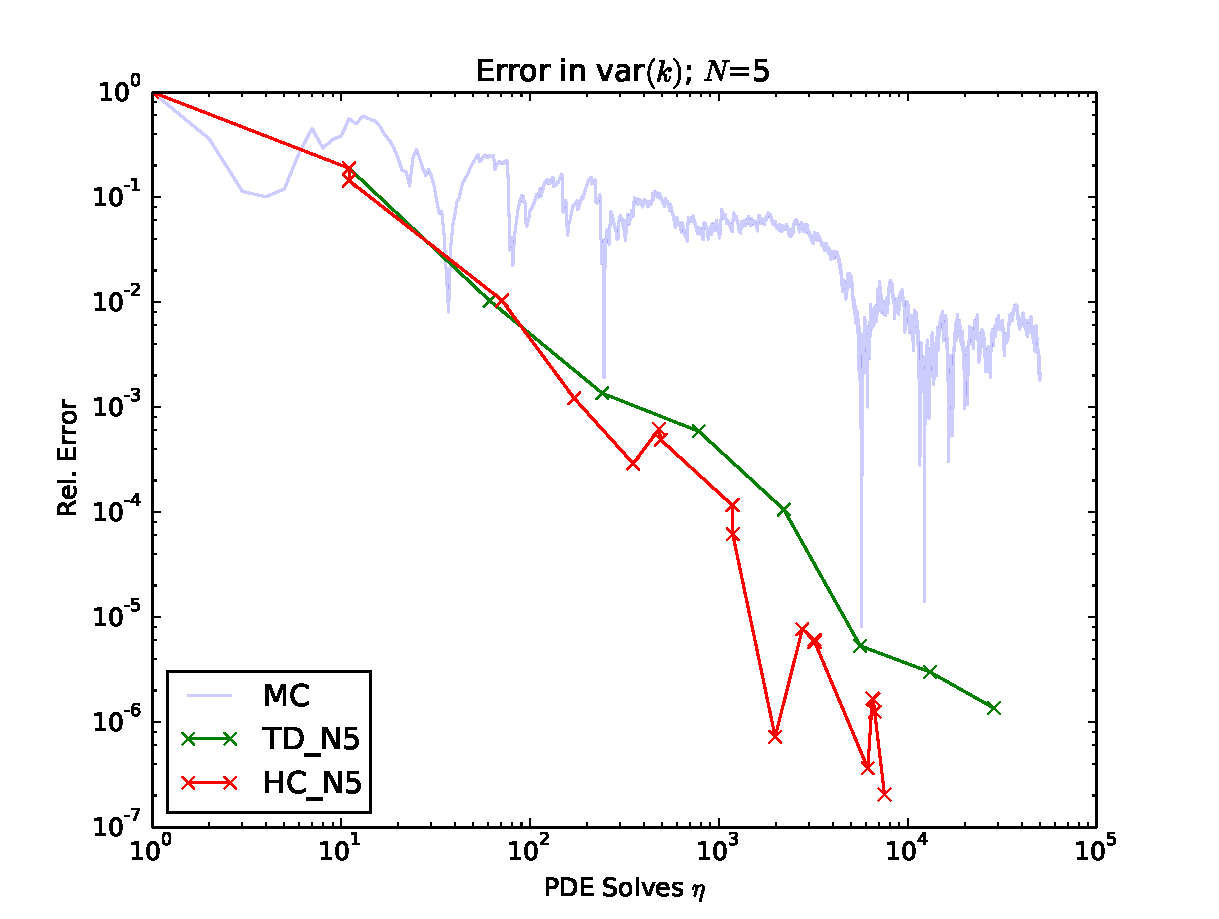
\includegraphics[width=\textwidth]{../graphics/N5_iso_var_errs}
   \caption{Errors}
   \label{n5var}
  \end{subfigure}
  \caption{Diffusion, $N=5$, Variance}
  \label{n5}
\end{figure}

\begin{figure}[h]
\centering
  \begin{subfigure}[b]{0.49 \textwidth}
   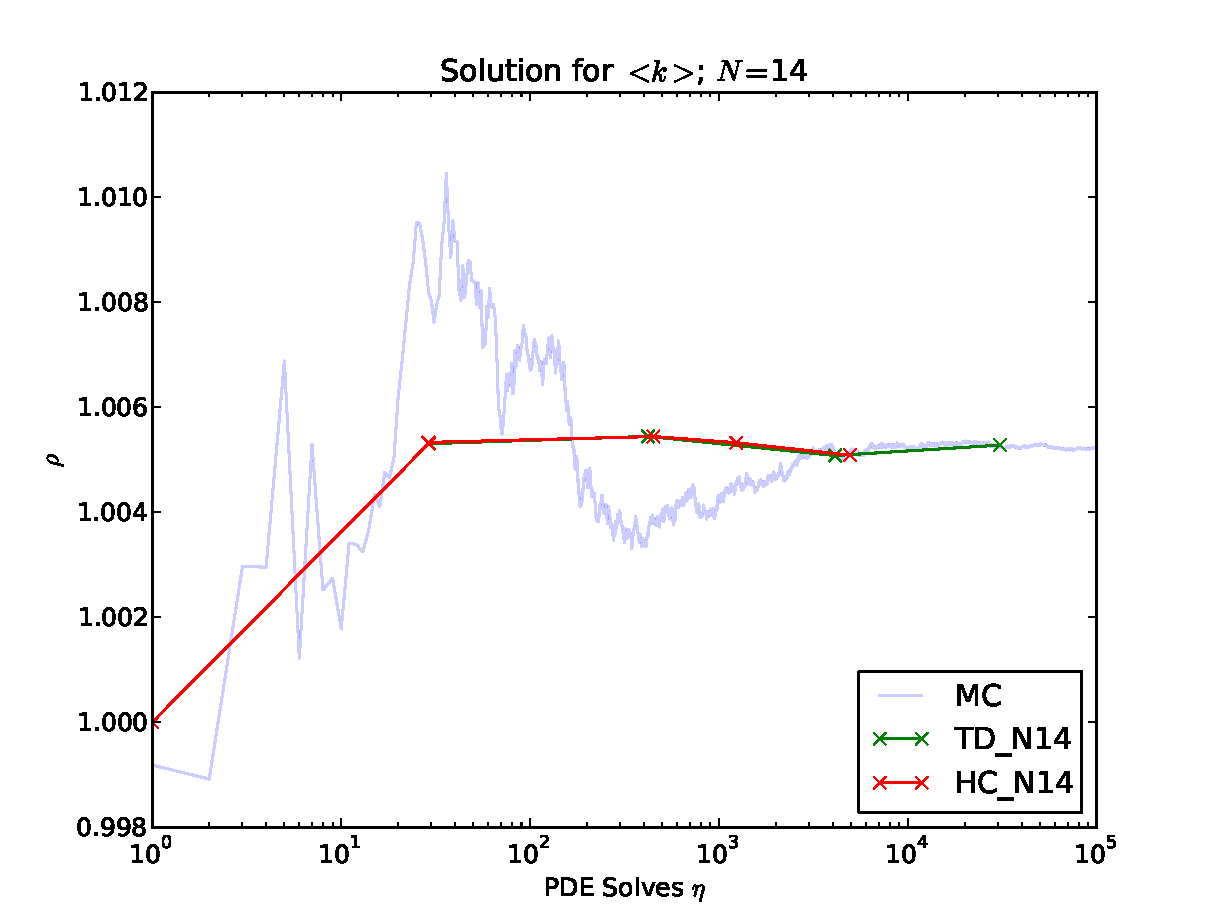
\includegraphics[width=\textwidth]{../graphics/soln_14}
   \caption{Values}
   \label{n14mean}
  \end{subfigure}
  \begin{subfigure}[b]{0.49 \textwidth}
   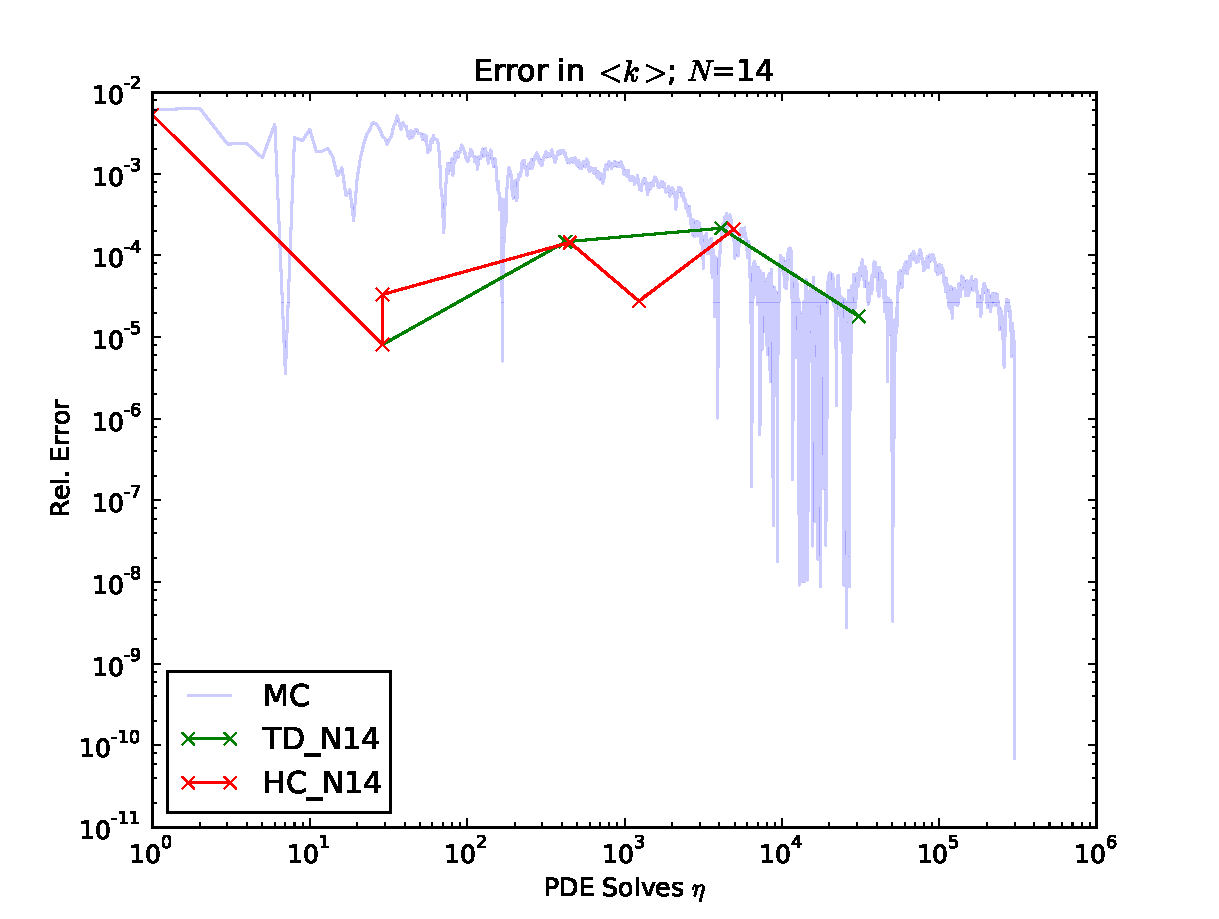
\includegraphics[width=\textwidth]{../graphics/err_14}
   \caption{Errors}
   \label{n14mean}
  \end{subfigure}
  \caption{Diffusion, $N=14$, Mean}
  \label{n14}
\end{figure}

\begin{figure}[h]
\centering
  \begin{subfigure}[b]{0.49 \textwidth}
   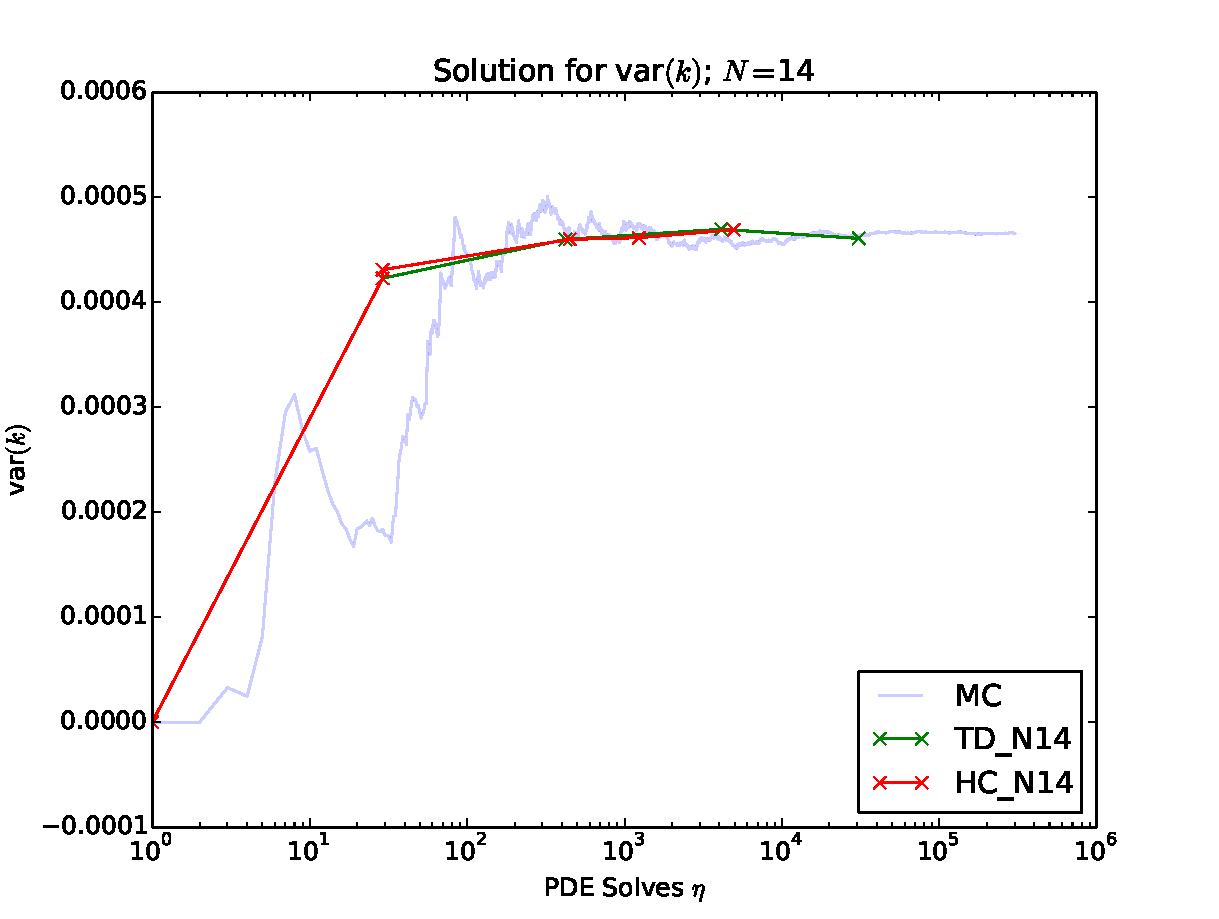
\includegraphics[width=\textwidth]{../graphics/N14_iso_var_vals}
   \caption{Values}
   \label{n14var}
  \end{subfigure}
  \begin{subfigure}[b]{0.49 \textwidth}
   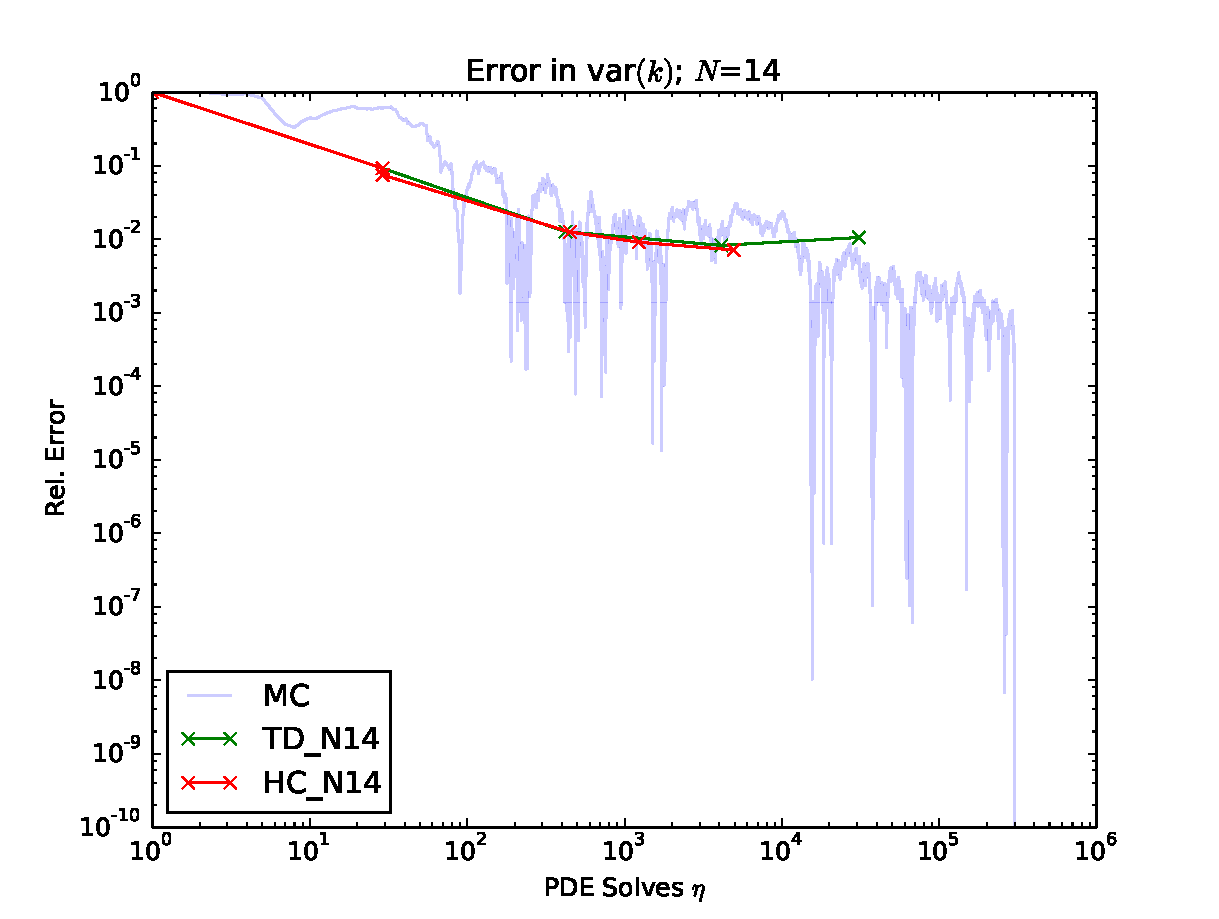
\includegraphics[width=\textwidth]{../graphics/N14_iso_var_errs}
   \caption{Errors}
   \label{n14var}
  \end{subfigure}
  \caption{Diffusion, $N=14$ Variance}
  \label{n14}
\end{figure}

%%%%%%%%%%%%%%%%%%%%%%%%%%%%%%%%%%
%%%%%%%%%%%%%%%%%%%%%%%%%%%%%%%%%%
%%%%%%%%%%%%%%%%%%%%%%%%%%%%%%%%%%

\section{Additional Improvements}
Besides using sparse grid quadrature for stochastic collocation, there are a number of other approaches to stochastic collocation that can further reduce the sample space and improve convergence.

\subsection{Anisotropic Sparse Grid}
One disadvantage of sparse grids as defined above is that it treats all dimensions of uncertainty space equally.  In many cases, however, the sensitivity of the stochastic solution to one dimension is less than another.  For example, we heuristically expect the sensitivity of the $k$-eigenvalue to the reflecting material (material 5) diffusion coefficient to be much less than the sensitivity to the fission cross section in the main fissile material (material 1).  

We can leverage the varying sensitivity by introducing importance parameters $\vec\alpha=[\alpha_1,\cdots,\alpha_N]$ that parametrize the sensitivity of the stochastic solution to each dimension.  Using the one-norm
\begin{equation}
\qty|\vec\alpha|_1\equiv\frac{1}{N}\sum_{n=1}^N \alpha_n,
\end{equation}
these weight parameters adjust the index set rules $\Lambda(L)$ for total degree and hyperbolic cross as
\begin{equation}
\tilde\Lambda_\text{TD}(L)=\Big\{\bar p=[p_1,...,p_N]:\sum_{n=1}^N \alpha_n p_n \leq \qty|\vec\alpha|_1 L \Big\},
\end{equation}
\begin{equation}
\tilde\Lambda_\text{HC}(L)=\Big\{\bar p=[p_1,...,p_N]:\prod_{n=1}^N \qty(p_n+1)^{\alpha_n} \leq \qty(L+1)^{\qty|\vec\alpha|_1} \Big\}.
\end{equation}
In this formulation, greater values of $\alpha_n$ result in less quadrature points for uncertain input $Y_n$.  Smaller values of $\alpha_n$ are assigned to more sensitive dimensions to prioritize collocation points.


\subsection{HDMR}
Despite the gains in efficiency from using anisotropic sparse grids, stochastic collocation still suffers from the curse of dimensionality, becoming computationally unwieldy for more than a dozen uncertain inputs.  We can further improve the efficiency of deterministic uncertainty quantification by making use of high-density model reduction (HDMR) techniques \cite{hdmr}.  These methods have been applied recently to neutronics problems for significant gain in efficiency \cite{hdmr_neutron}.

Cut-HDMR makes use of representative ``slices'' or cuts of the uncertainty space.  This slice in uncertainty space makes use of ``reference values'' for each of the uncertain inputs, often the mean or most likely value for the parameter.  We denote the reference value for input parameter $Y_n$ as $Y_n^{(0)}$.  Cut-HDMR uses reference values for the majority of inputs at a time and varies small numbers of parameters, then constructs the results as a linear sum of the contributions.
It approximates a function as a sum of increasing interactions,
\begin{equation}
u(Y)= H[u](Y)=u_0 + \sum_{n_1=1}^N u_{n_1} + \sum_{n_1=1}^N\sum_{n_2=1}^{n_1} u_{n_1,n_2} + 
                     \sum_{n_1=1}^N\sum_{n_2=1}^{n_1}\sum_{n_3=1}^{n_2}u_{n_1,n_2,n_3}+...,
\end{equation}
\begin{equation}
u_0=u(Y^{(0)}),
\end{equation}
\begin{equation}
u_{n}\equiv u(Y_n) - u_0,
\end{equation}
\begin{equation}
u_{i,j}\equiv u(Y_i,Y_j,\bar Y) - u_i - u_j - u_0,
\end{equation}
and so on.  Here $N$ is the total number of uncertain inputs, and 
\begin{equation}
u(Y_{n})=u\big|_{Y_i=Y_i^{(0)},i\neq n}\equiv u(Y_1^{(0)},Y_2^{(0)},\ldots,Y_n,\ldots,Y_N^{(0)}),
\end{equation}
indicates holding any variables not explicitly listed at the reference value.  For multiple listed uncertain inputs,
\begin{equation}
u(Y_m,Y_{n})\equiv u(Y_1^{(0)},Y_2^{(0)},\ldots,Y_m,\ldots,Y_n,\ldots,Y_N^{(0)}),
\end{equation}
This Cut-HDMR representation allows us to approximate by truncating at a particular interaction level $H$.  For instance, an $H2$ approximation would only include the terms
\begin{equation}
u(Y)\approx H_2[u](Y) = u_0 + \sum_i^N u_i + \sum_i^N\sum_j^{i-1} u_{i,j}.
\end{equation}
A variety of methods can be used to represent $u(Y)$.  In our case, we make use of stochastic collocation on sparse grids, which is most efficient for a moderate number of uncertain inputs.  For example,
\begin{equation}
u(Y)\approx H_2[u](Y)\approx S_0 + \sum_i^N S_i + \sum_i^N\sum_j^{i-1} S_{i,j},
\end{equation}
\begin{equation}
S_0\equiv S[u](\bar Y),
\end{equation}
\begin{equation}
S_i\equiv S[u](Y_i,\bar Y) - S_0,
\end{equation}
\begin{equation}
S_{i,j}\equiv S[u](Y_i,Y_j,\bar Y) - S_i - S_j - S_0.
\end{equation}
Moments $r$ of this HDMR approximation can be obtained simply as - TODO is this true? - 
\begin{equation}
\expv{u(Y)^r}=\expv{H[u](Y)^r}=u_0^r + \sum_i^N u_i^r + \sum_i^N\sum_j^i u_{i,j}^r+...
\end{equation}

\subsubsection{Attenuation Problem Results}
Figures \ref{atn vals hdmr} and \ref{atn errs hdmr} compare the convergence of the additional methods described here as a function of the number of deterministic solves required.  Because each variable contributes identically, anisotropic methods did not show any improvement over collocation and are omitted for this problem.  We note that, for five input parameters, it appears HDMR at best can tie the uncertainty convergence obtained by full collocation.  This is sensible, as using sparse grid quadrature already removes most of the higher-order interactions between variables from consideration.  We expect that as the number of input parameters increases, the benefit of HDMR will as well.
\begin{figure}[h]
    \centering
    \begin{subfigure}[b]{0.49 \textwidth}
      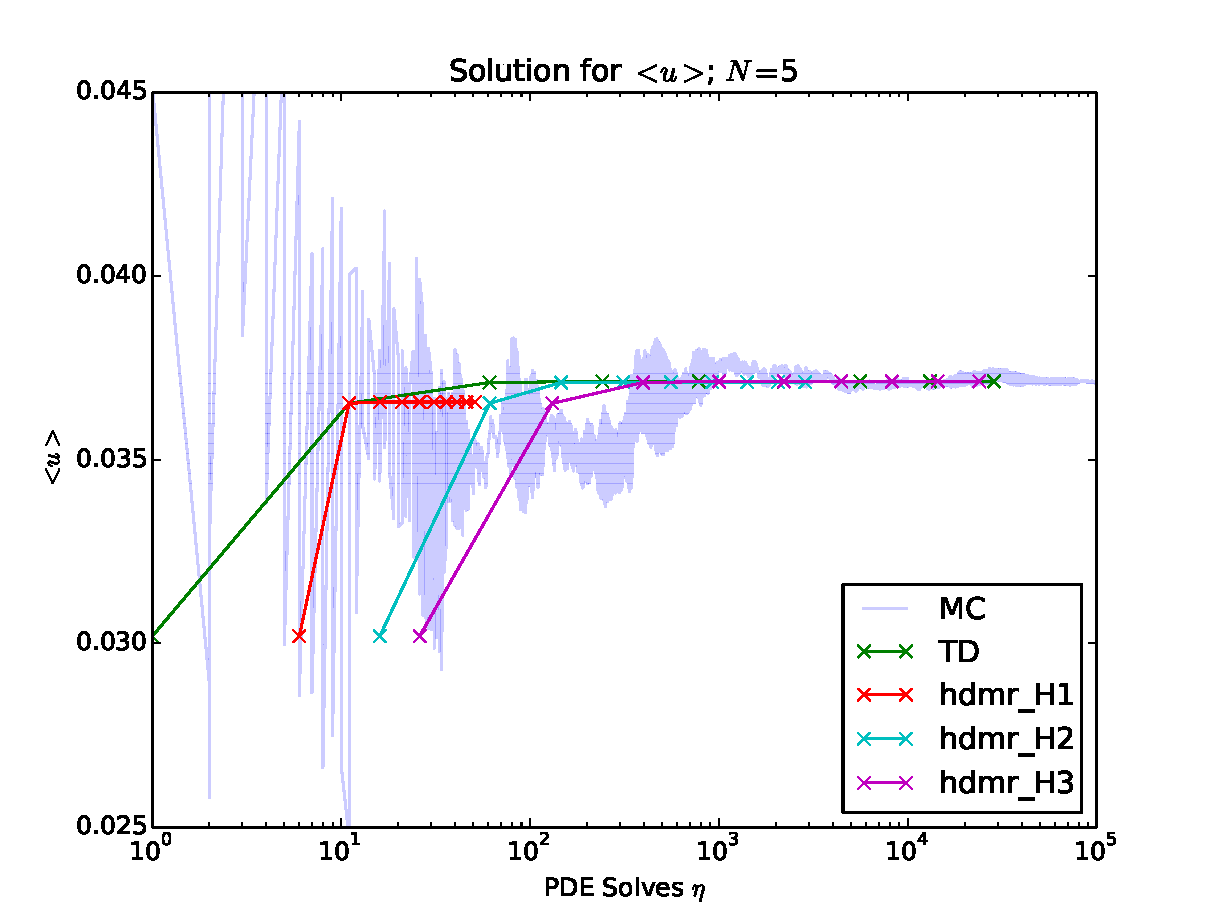
\includegraphics[width=\textwidth]{../graphics/attenuate_N5_soln_hdmr}
      \caption{$<u>$ Values}
      \label{atn vals hdmr}
  \end{subfigure}
\begin{subfigure}[b]{0.49 \textwidth}
\centering
      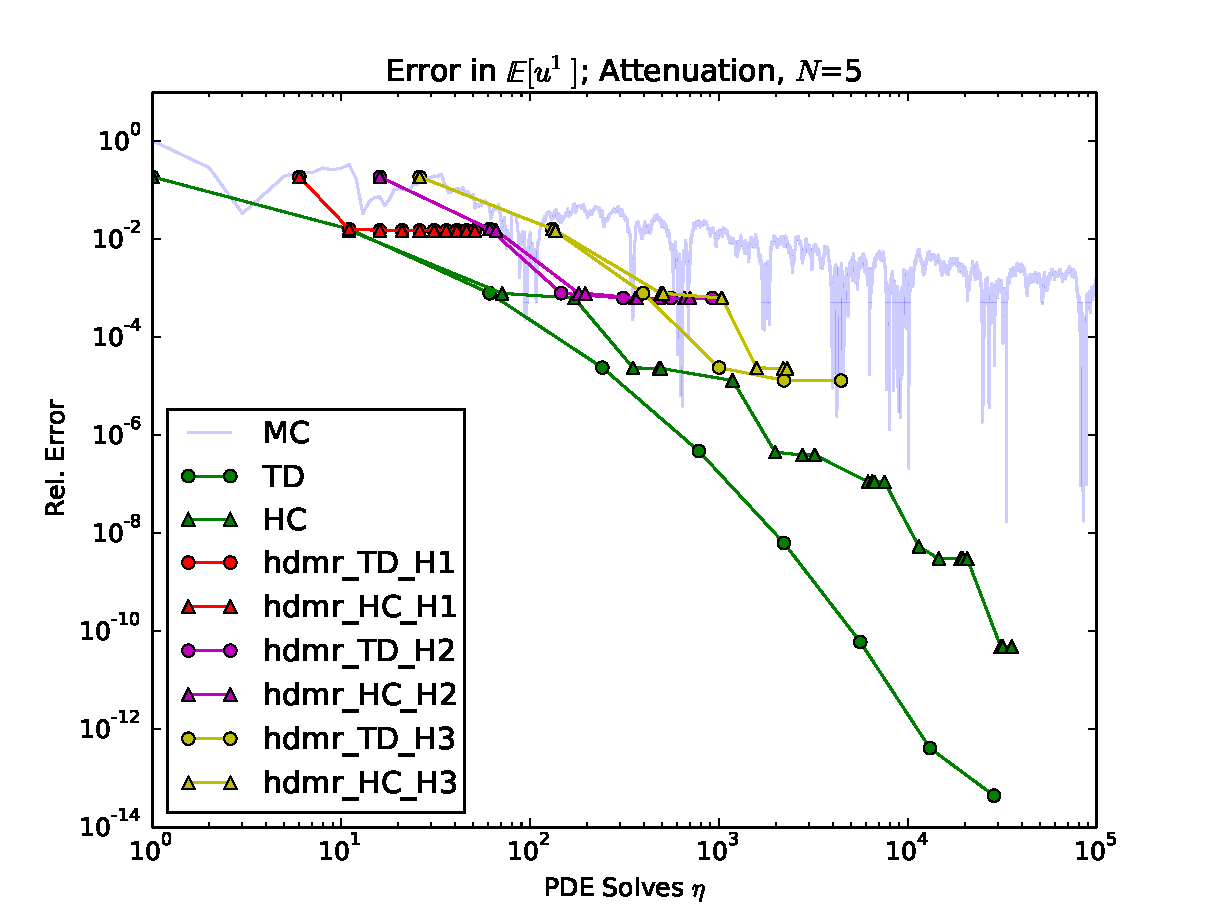
\includegraphics[width=\textwidth]{../graphics/attenuate_N5_conv_hdmr}
      \caption{Error in $<u>$}
      \label{atn errs hdmr}
    \end{subfigure}
  \caption{Attenuation UQ Results, Mean}
  \label{atn results}
  \end{figure}

\begin{figure}[h]
    \centering
    \begin{subfigure}[b]{0.49 \textwidth}
      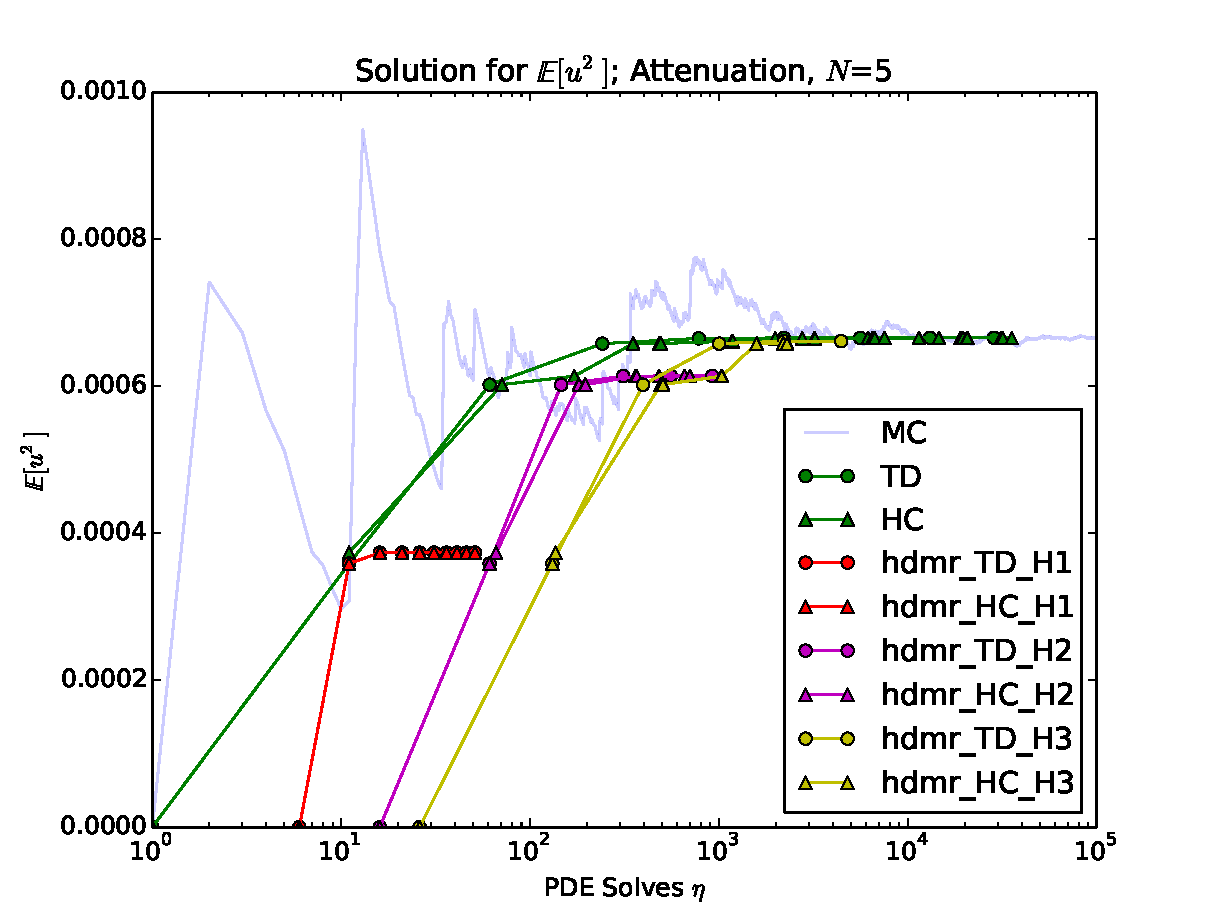
\includegraphics[width=\textwidth]{../graphics/attenuate_N5_soln_hdmr_variance}
      \caption{$<u>$ Values}
      \label{atn vals hdmr}
  \end{subfigure}
\begin{subfigure}[b]{0.49 \textwidth}
\centering
      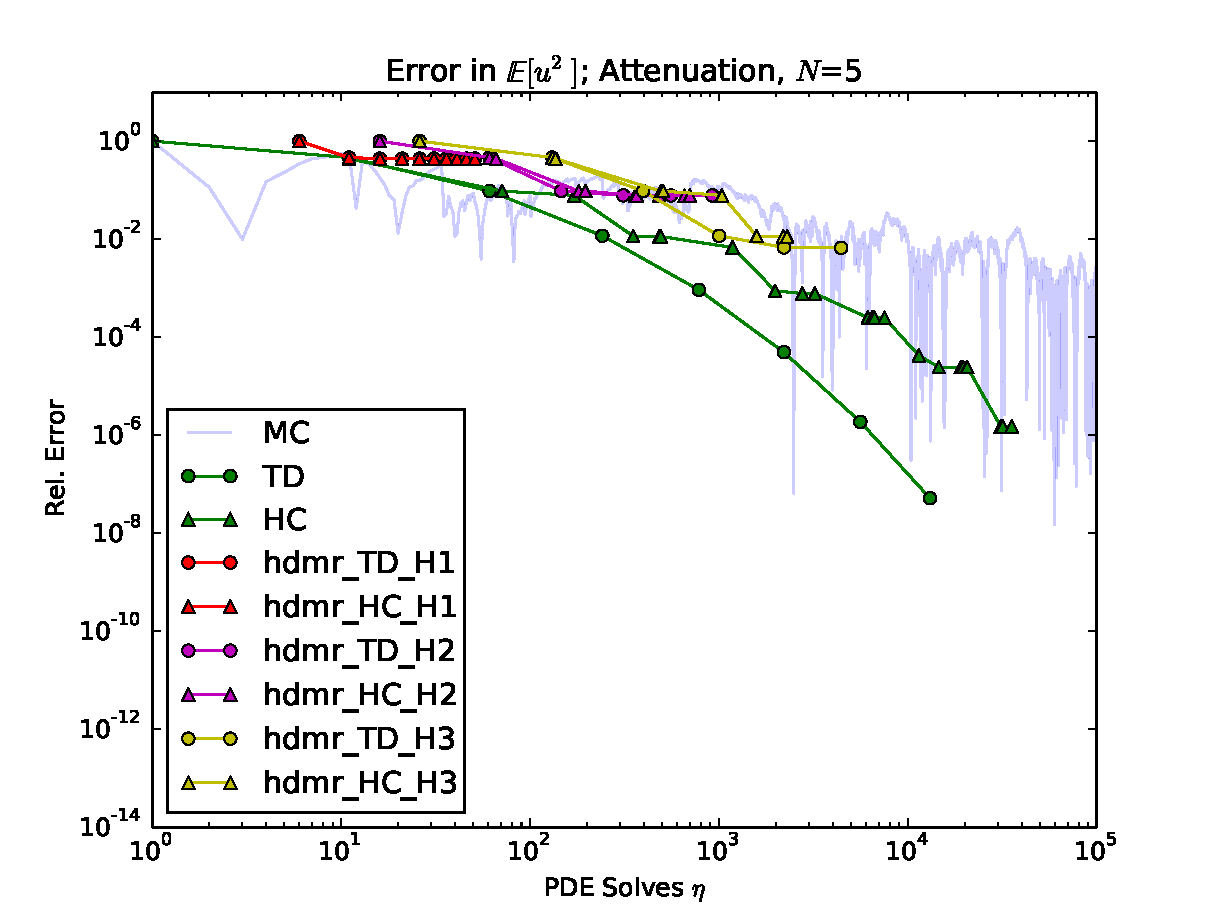
\includegraphics[width=\textwidth]{../graphics/attenuate_N5_conv_hdmr_variance}
      \caption{Error in $<u>$}
      \label{atn errs hdmr}
    \end{subfigure}
  \caption{Attenuation UQ Results, Variance}
  \label{atn results}
  \end{figure}


\subsubsection{Projectile Problem Results}
\begin{figure}[h]
    \centering
    \begin{subfigure}[b]{0.49 \textwidth}
      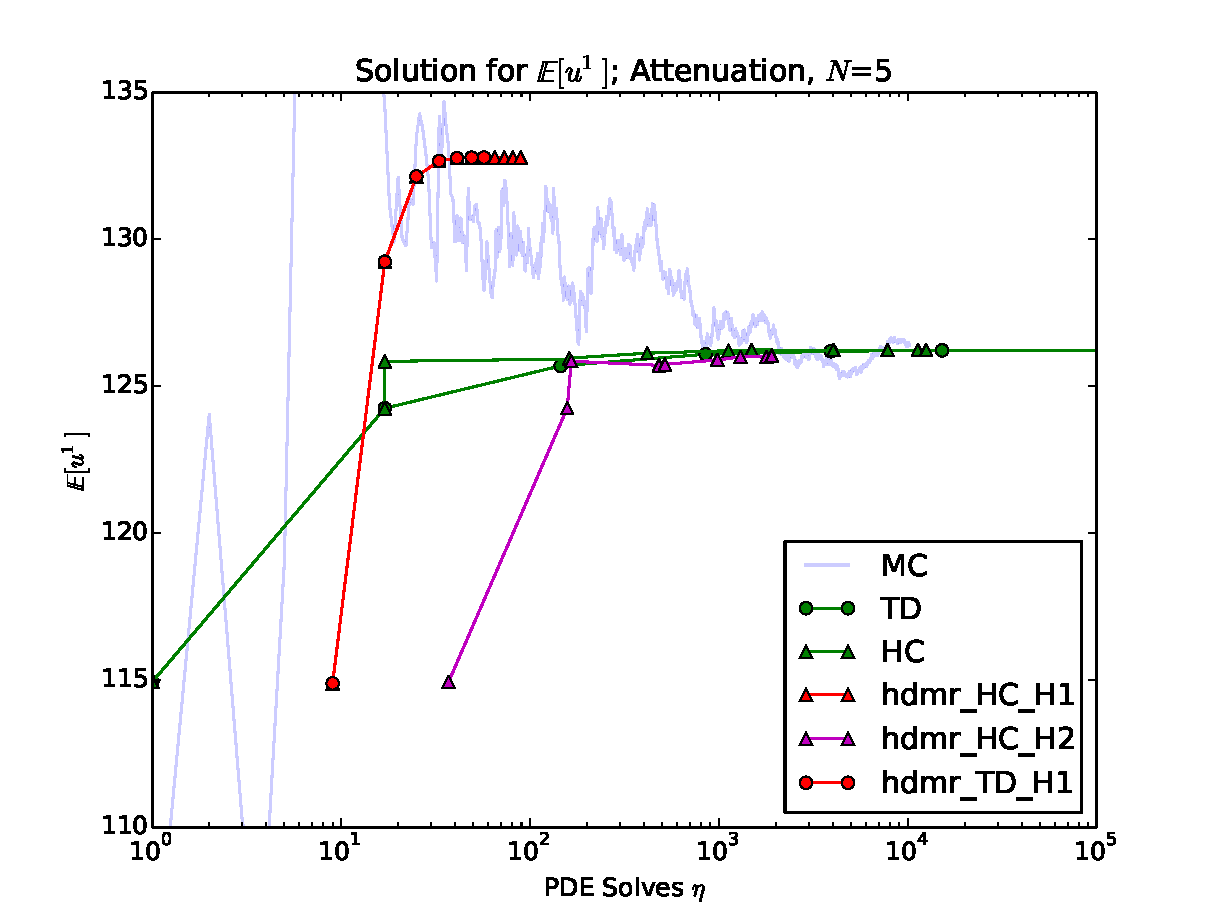
\includegraphics[width=\textwidth]{../graphics/projectile_solns_hdmr}
      \caption{$<u>$ Values}
      \label{atn vals hdmr}
  \end{subfigure}
\begin{subfigure}[b]{0.49 \textwidth}
\centering
      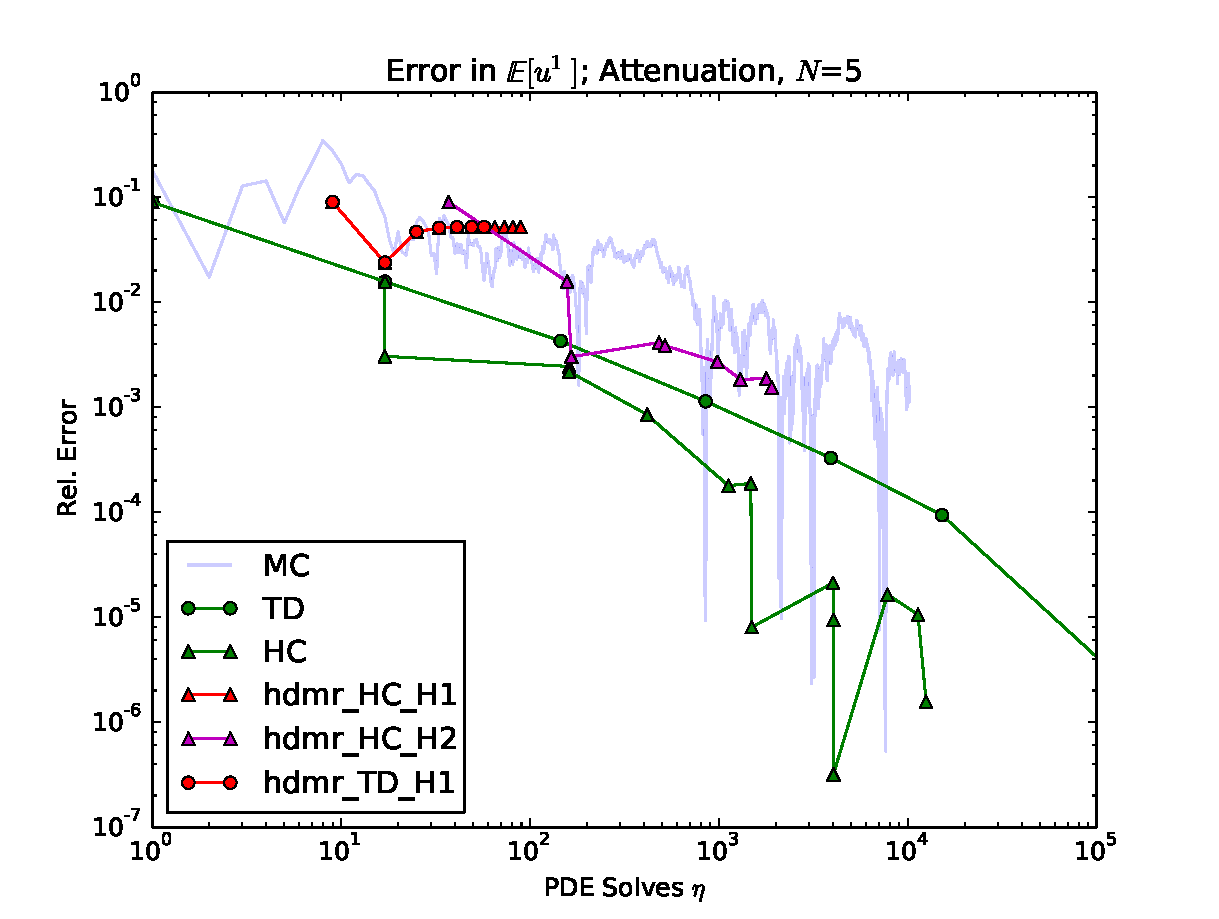
\includegraphics[width=\textwidth]{../graphics/projectile_errs_hdmr}
      \caption{Error in $<u>$}
      \label{atn errs hdmr}
    \end{subfigure}
  \caption{Projectile UQ Results, Mean}
  \label{atn results}
  \end{figure}

\begin{figure}[h]
    \centering
    \begin{subfigure}[b]{0.49 \textwidth}
      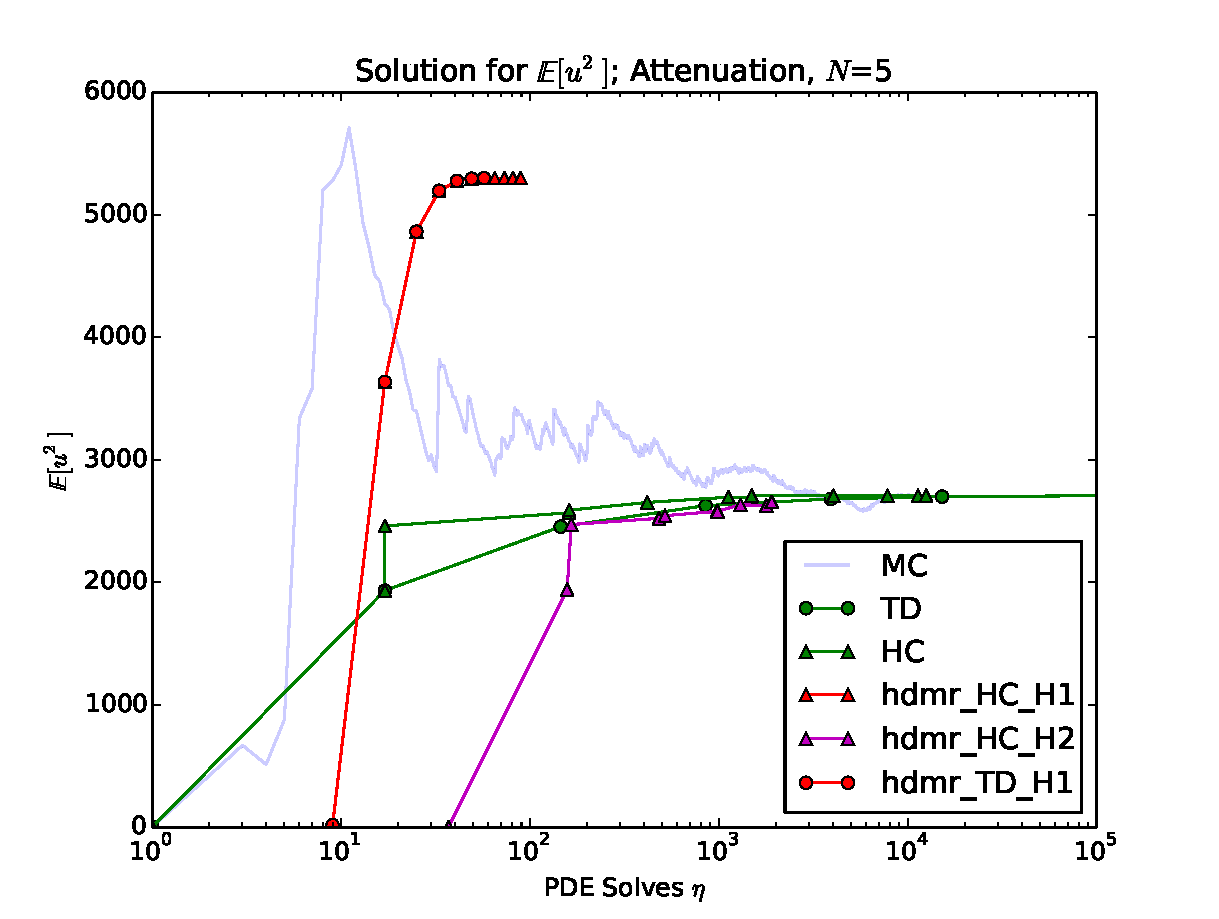
\includegraphics[width=\textwidth]{../graphics/projectile_solns_hdmr_variance}
      \caption{$<u>$ Values}
      \label{atn vals hdmr}
  \end{subfigure}
\begin{subfigure}[b]{0.49 \textwidth}
\centering
      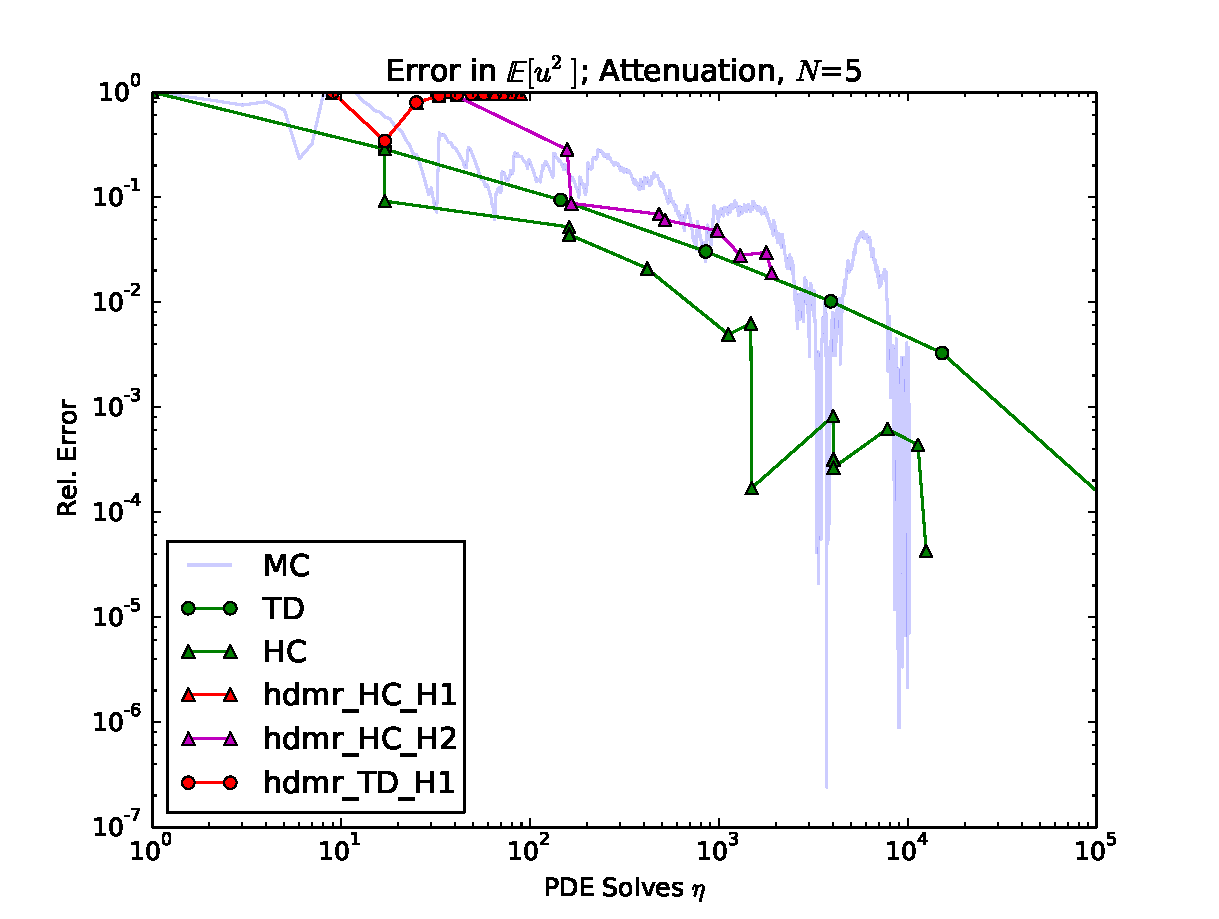
\includegraphics[width=\textwidth]{../graphics/projectile_errs_hdmr_variance}
      \caption{Error in $<u>$}
      \label{atn errs hdmr}
    \end{subfigure}
  \caption{Projectile UQ Results, Variance}
  \label{atn results}
  \end{figure}



\subsubsection{Diffusion Problem Results}
%\begin{figure}[H]
%    \centering
%    \begin{subfigure}[b]{0.49 \textwidth}
%      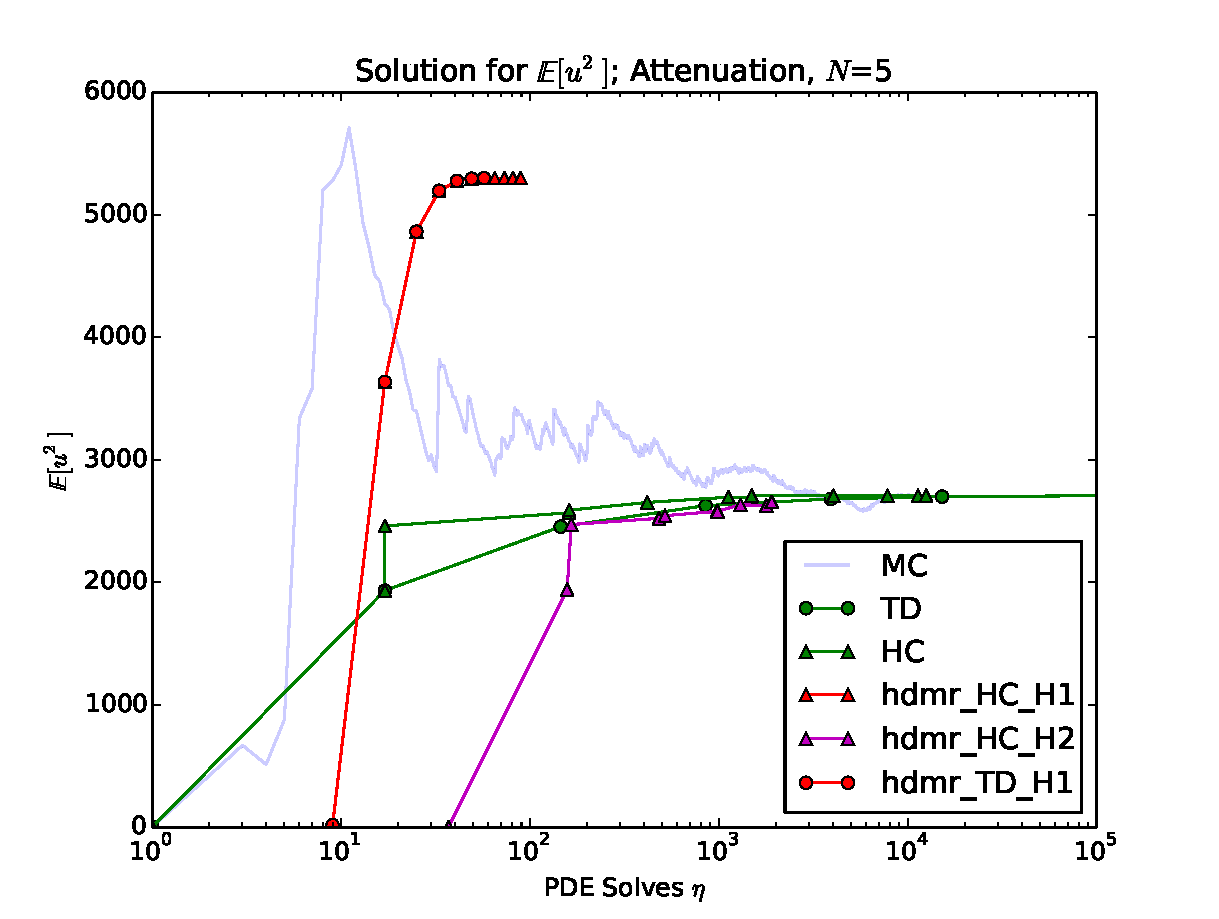
\includegraphics[width=\textwidth]{../graphics/projectile_solns_hdmr_variance}
%      \caption{$<u>$ Values}
%      \label{atn vals hdmr}
%  \end{subfigure}
%\begin{subfigure}[b]{0.49 \textwidth}
%\centering
%      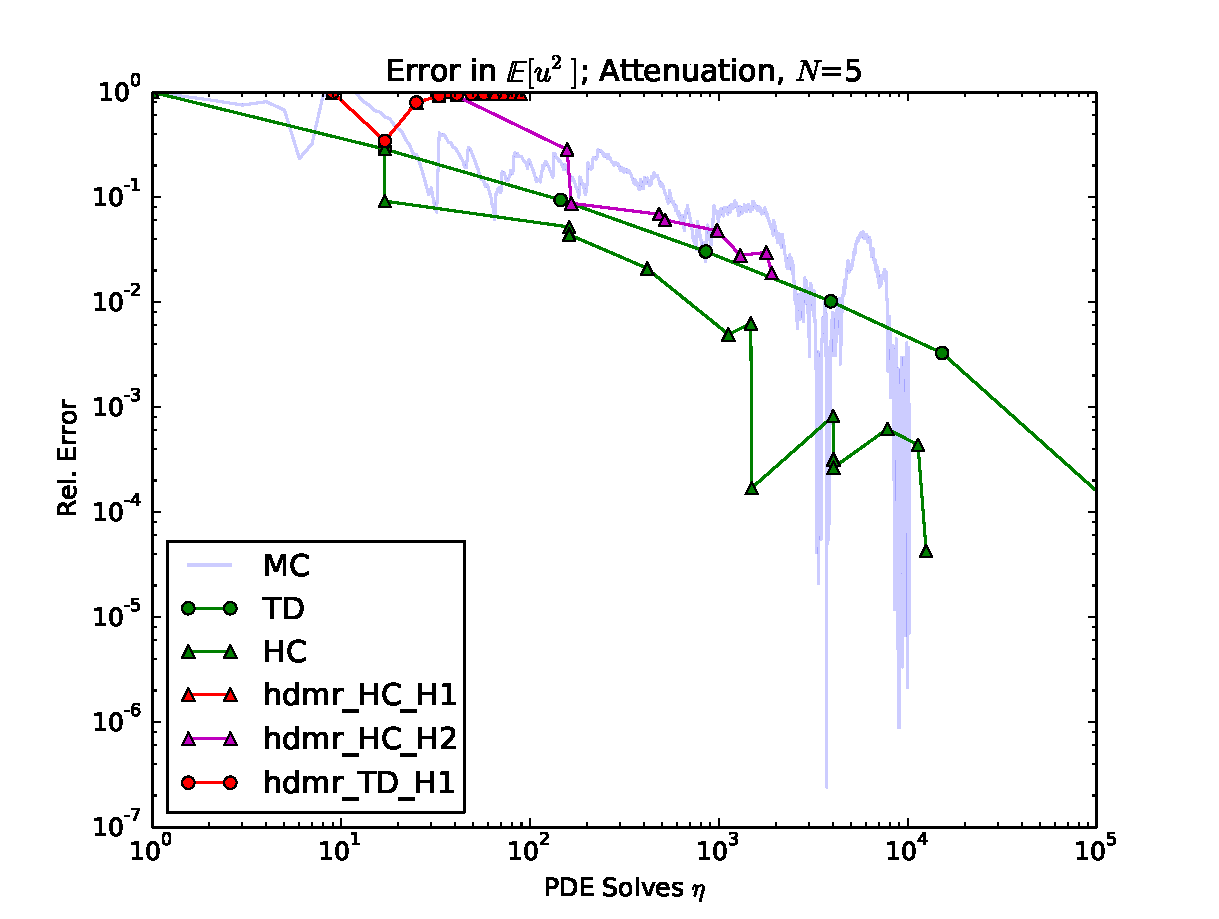
\includegraphics[width=\textwidth]{../graphics/projectile_errs_hdmr_variance}
%      \caption{Error in $<u>$}
%      \label{atn errs hdmr}
%    \end{subfigure}
%  \caption{Projectile UQ Results, Variance}
%  \label{atn results}
%  \end{figure}



\subsection{Anisotropic Sparse Grid}
One disadvantage of sparse grids as defined above is that it treats all dimensions of uncertainty space equally.  In many cases, however, the sensitivity of the stochastic solution to one dimension is less than another.  For example, we heuristically expect the sensitivity of the $k$-eigenvalue to the reflecting material (material 5) diffusion coefficient to be much less than the sensitivity to the fission cross section in the main fissile material (material 1).  

We can leverage the varying sensitivity by introducing importance parameters $\vec\alpha=[\alpha_1,\cdots,\alpha_N]$ that parametrize the sensitivity of the stochastic solution to each dimension.  Using the one-norm
\begin{equation}
\qty|\vec\alpha|_1\equiv\frac{1}{N}\sum_{n=1}^N \alpha_n,
\end{equation}
these weight parameters adjust the index set rules $\Lambda(L)$ for total degree and hyperbolic cross as
\begin{equation}
\tilde\Lambda_\text{TD}(L)=\Big\{\bar p=[p_1,...,p_N]:\sum_{n=1}^N \alpha_n p_n \leq \qty|\vec\alpha|_1 L \Big\},
\end{equation}
\begin{equation}
\tilde\Lambda_\text{HC}(L)=\Big\{\bar p=[p_1,...,p_N]:\prod_{n=1}^N \qty(p_n+1)^{\alpha_n} \leq \qty(L+1)^{\qty|\vec\alpha|_1} \Big\}.
\end{equation}
In this formulation, greater values of $\alpha_n$ result in less quadrature points for uncertain input $Y_n$.  Smaller values of $\alpha_n$ are assigned to more sensitive dimensions to prioritize collocation points.

One method to quantify the sensitivity of the quantity of interest to changes in each input parameter is by using an ANOVA-like approach with a well-converged HDMR calculation.  We derive an importance factor based on the contribution of each single variable to the overall second moment.
\begin{equation}
\expv{u(Y)^2} \approx \expv{H_3[u](Y)^2} =
                    u_0^2 + \sum_{n_1=1}^N u_{n_1}^2 + \sum_{n_1=1}^N\sum_{n_2=1}^{n_1} u_{n_1,n_2}^2 + 
                     \sum_{n_1=1}^N\sum_{n_2=1}^{n_1}\sum_{n_3=1}^{n_2}u_{n_1,n_2,n_3}^2,
\end{equation}
\begin{equation}
\alpha_n = \text{ceil}\left[-\log\left(\frac{u_n^2}{\expv{H[u](Y)^2}}\right)\right].
\end{equation}
While not the only method for calculating weight factors, this formulation ensures positive integers with a minimum of 1 for each weight factor.

We omit results for the attenuation case, as each variable contributes identically and no anisotropy performs better than isotropic sparse grid for this case.

\subsubsection{Projectile Problem}
Table \ref{tab:proj anis} shows values found using an order $H_1[u](Y)$ approximation for the projectile problem.  The drag coefficient $C$ is clearly the input with the most impact, while the gravitational acceleration constant $g$ has the least effect.  We note that these sensitivities are based on the uncertain ranges given above; changing the uncertainty ranges or distribution could impact the weighting factors $\alpha$.  As shown in Figures \ref{proj anis mean} and \ref{proj anis variance}, employing a variance-based anisotropic sparse grid collocation shows orders of magnitude improvement in convergence and overall error when compared to isotropic sparse grid collocation.
\begin{table}[h]
\centering
\begin{tabular}{c|c c|c}
$Y_n$ & $Y_n^2$ & $\frac{Y_n^2}{H_1^2[u](Y)}$ & $\alpha_n$ \\ \hline
$m$ & 2.57E4 & 6.2E-5 & 5 \\
$r$ & 2.61E4 & 6.3E-5 & 5 \\
$C$ & 9.45E7 & 2.3E-1 & 1 \\
$\rho$ & 1.52E3 & 3.6E-6 & 6 \\
$v$ & 4.18E1 & 1.0E-7 & 7 \\
$\theta$ & 1.93E7 & 4.6E-2 & 2 \\
$g$ & 2.77E-3 & 6.6E-12 & 12 \\
$y_i$ & 1.56E4 & 5.7E-5 & 5
\end{tabular}
\caption{Anisotropies for Projectile Problem}
\label{tab:proj anis}
\end{table}
\begin{figure}[h]
    \centering
    \begin{subfigure}[b]{0.49 \textwidth}
      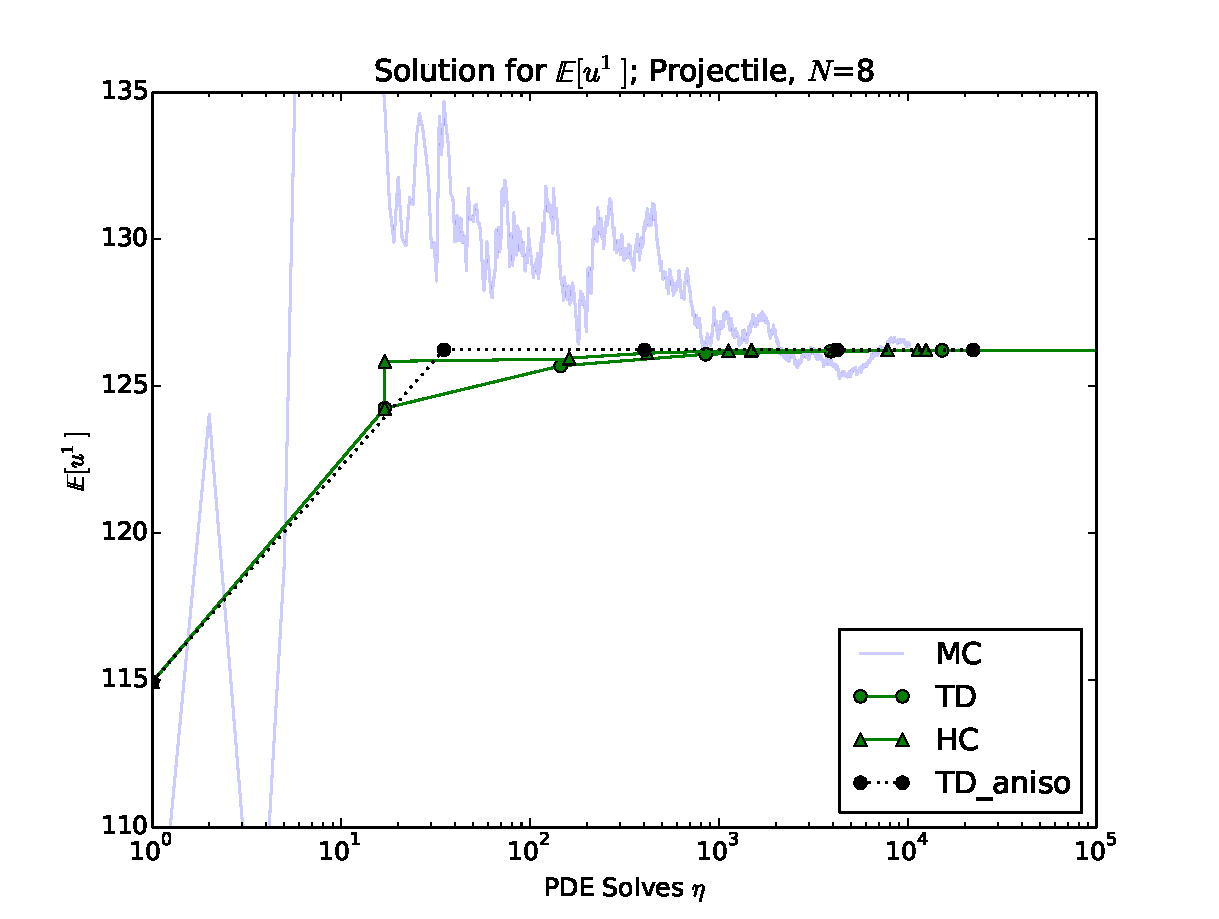
\includegraphics[width=\textwidth]{../graphics/projectile_solns_aniso}
      \caption{Values}
      \label{atn vals hdmr}
  \end{subfigure}
\begin{subfigure}[b]{0.49 \textwidth}
\centering
      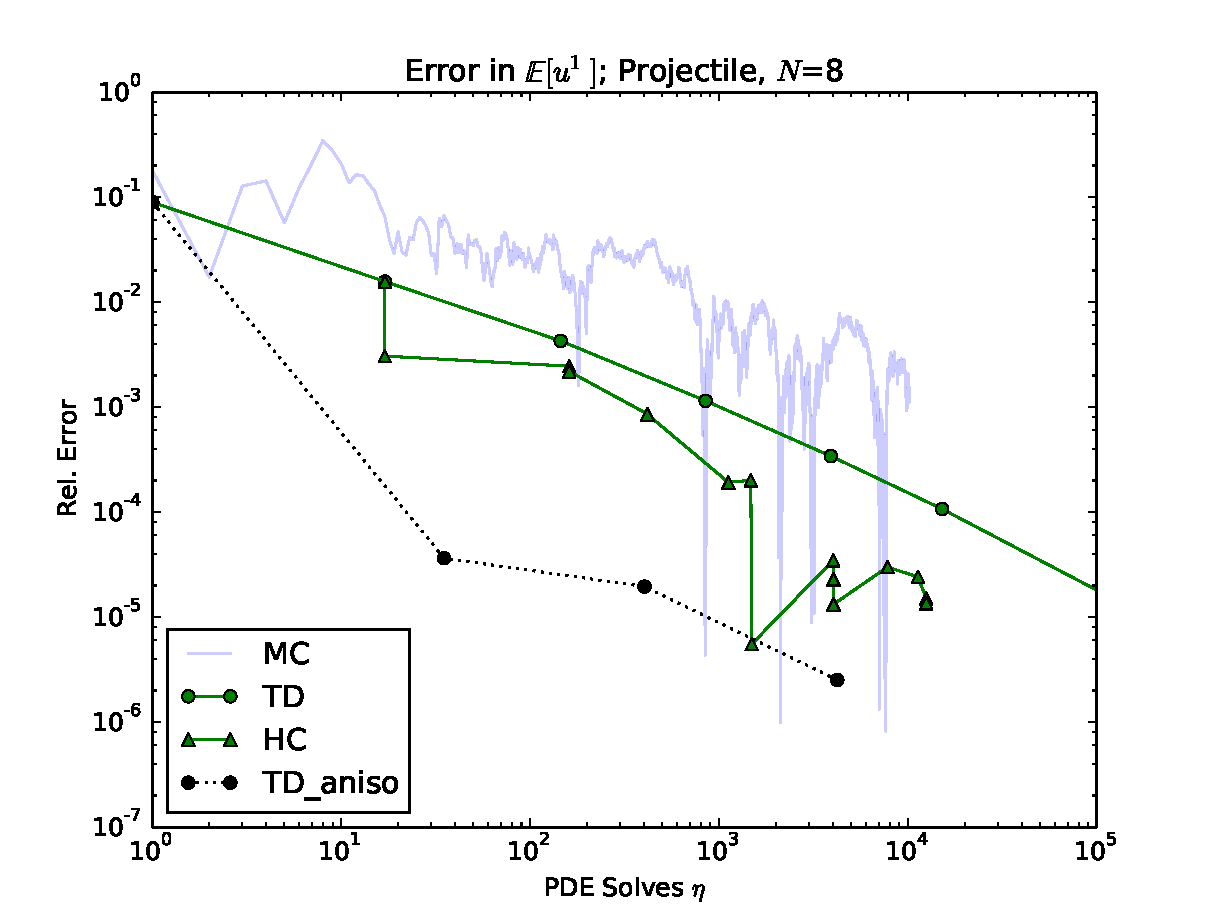
\includegraphics[width=\textwidth]{../graphics/projectile_errs_aniso}
      \caption{Error}
      \label{atn errs hdmr}
    \end{subfigure}
  \caption{Projectile UQ Results, Mean}
  \label{proj anis mean}
  \end{figure}

\begin{figure}[h]
    \centering
    \begin{subfigure}[b]{0.49 \textwidth}
      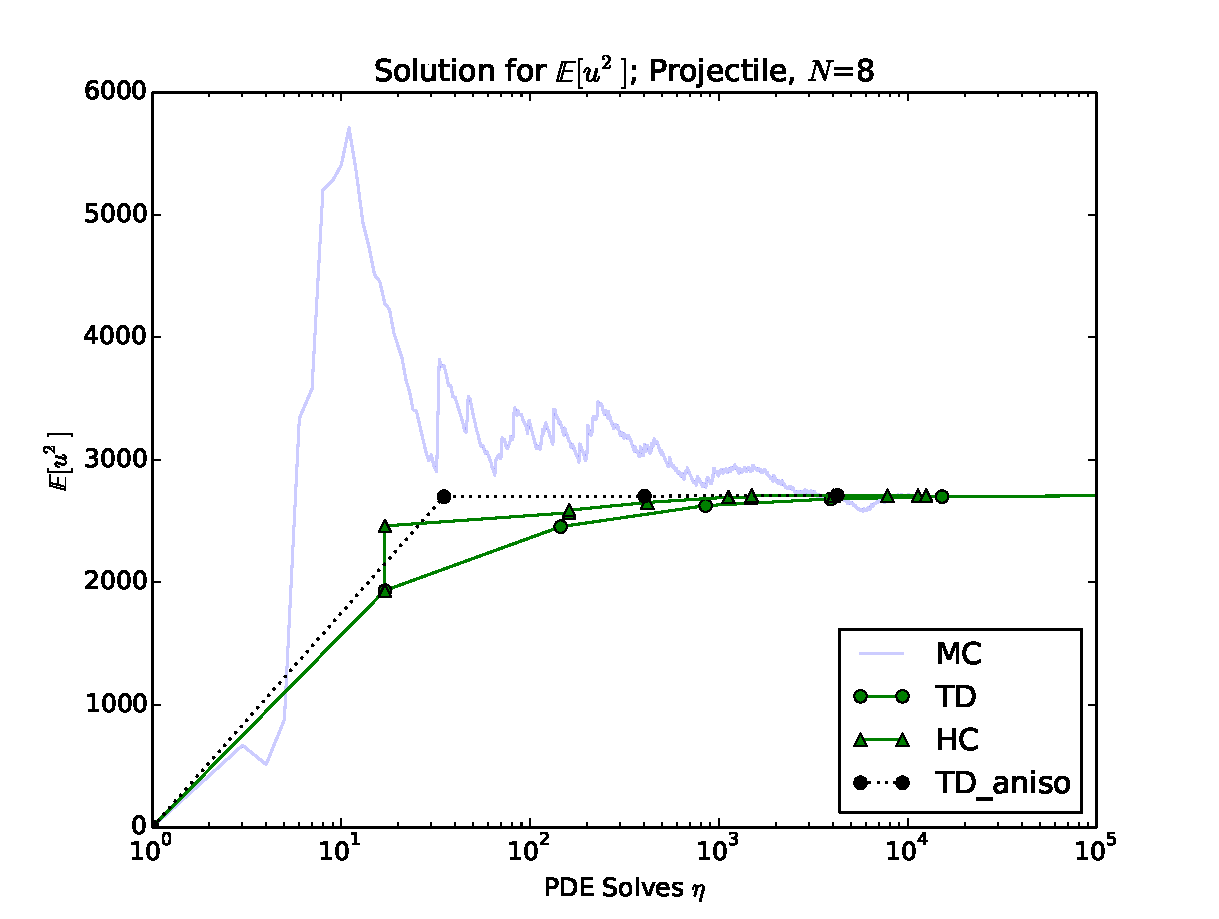
\includegraphics[width=\textwidth]{../graphics/projectile_solns_aniso_variance}
      \caption{Values}
      \label{atn vals hdmr}
  \end{subfigure}
\begin{subfigure}[b]{0.49 \textwidth}
\centering
      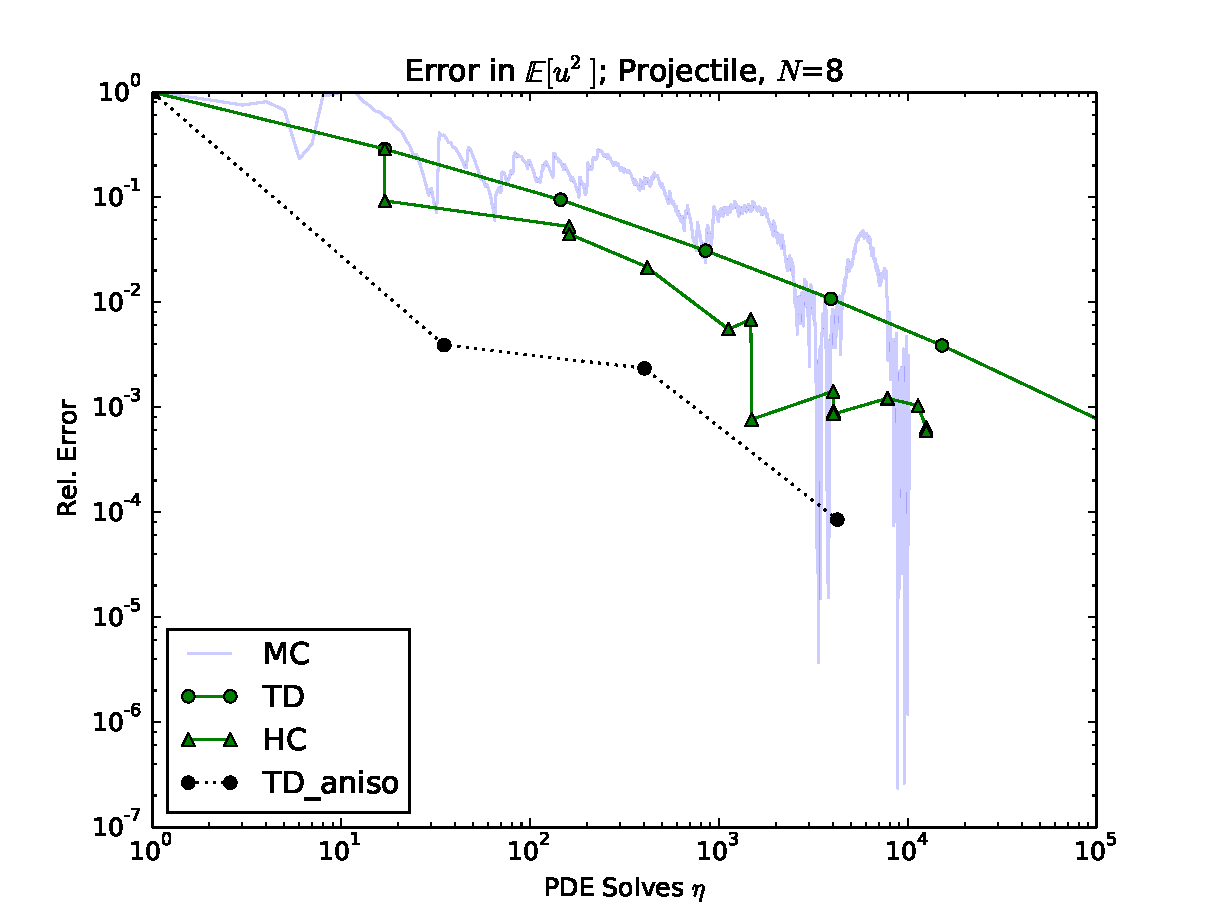
\includegraphics[width=\textwidth]{../graphics/projectile_errs_aniso_variance}
      \caption{Error}
      \label{atn errs hdmr}
    \end{subfigure}
  \caption{Projectile UQ Results, Variance}
  \label{proj anis variance}
  \end{figure}

\subsubsection{Diffusion Problem, $N=5$}
Table \ref{tab:diff5 anis} shows values found using an hdmr-based $H_1[u](Y)$ approximation for the diffusion problem.  As expected, the capture and fission cross sections in the most prevalent materials have the greatest effect on the $k$-eigenvalue.
As shown in Figures \ref{diff5 anis mean} and \ref{diff5 anis variance}, employing a variance-based anisotropic sparse grid collocation shows some improvement over an isotropic sparse grid.  There also is some indication of the resolution of the benchmark solution; the convergence of the mean becomes unstable around 10$^{-7}$ (10$^{-5}$ for the variance).  We expect a further-resolved benchmark would demonstrate continued convergence in all methods.

TODO Update table values with new ANOVA run

\begin{table}[h]
\centering
\begin{tabular}{c|c c|c}
$Y_n$ & $Y_n^2$ & $\frac{Y_n^2}{H_1^2[u](Y)}$ & $\alpha_n$ \\ \hline
$D^{(1)}_2$ & 1.75E-13 & 1.8E-13 & 13 \\
$\Sigma_{c,2}^{(1)}$ & 9.86E-6 & 9.9E-6 & 6 \\
$\Sigma_{f,2}^{(1)}$ & 4.80E-6 & 4.8E-6 & 6 \\
$D^{(4)}_2$ & 2.12E-14 & 2.1E-14 & 14 \\
$\Sigma_{c,2}^{(4)}$ & 2.05E-9 & 2.1E-9 & 9 \\
$\Sigma_{f,2}^{(4)}$ & 4.59E-10 & 4.6E-10 & 10 \\
$D^{(5)}_2$ & 6.18E-13 & 6.2E-13 & 13 
\end{tabular}
\caption{Anisotropies for Projectile Problem}
\label{tab:diff5 anis}
\end{table}
\begin{figure}[h]
    \centering
    \begin{subfigure}[b]{0.49 \textwidth}
      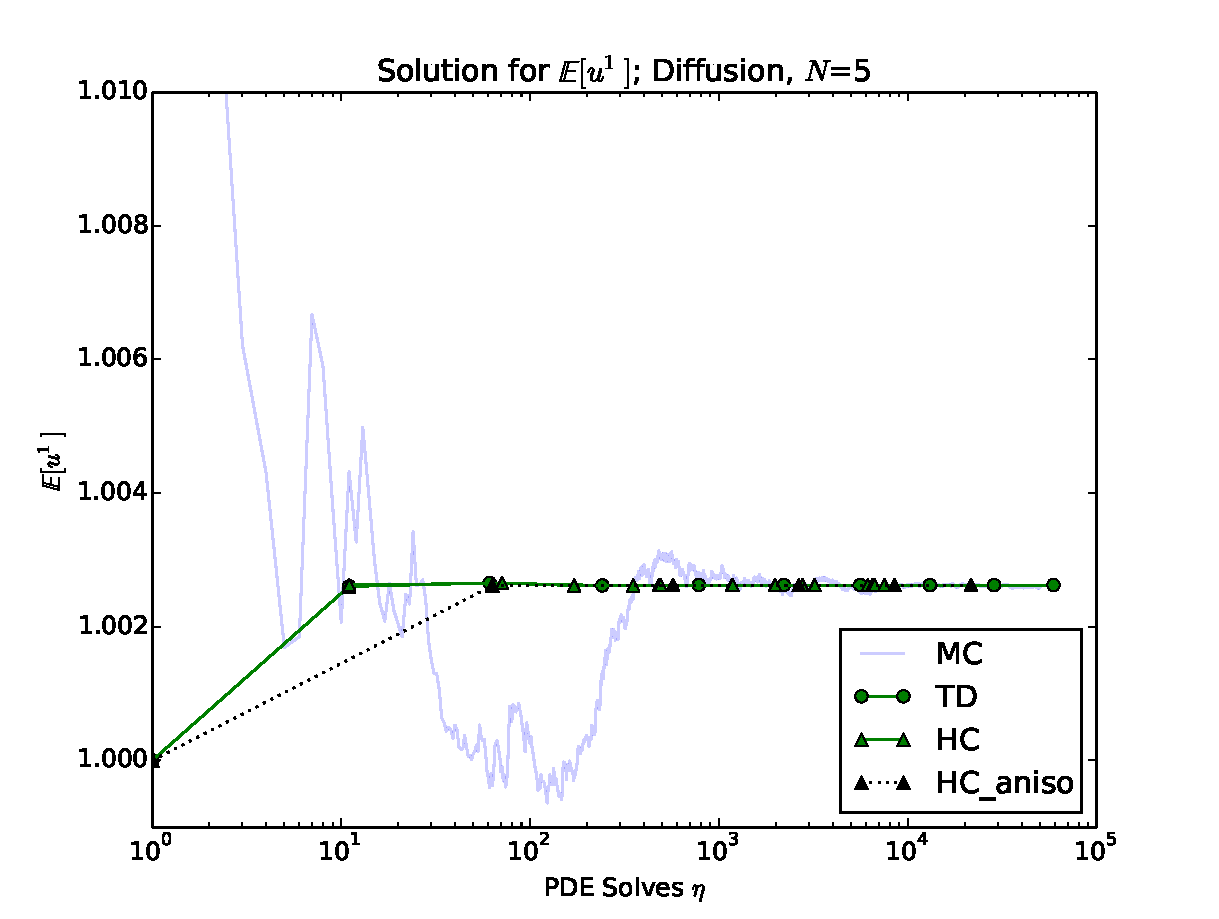
\includegraphics[width=\textwidth]{../graphics/N5_aniso_vals}
      \caption{Values}
      \label{atn vals hdmr}
  \end{subfigure}
\begin{subfigure}[b]{0.49 \textwidth}
\centering
      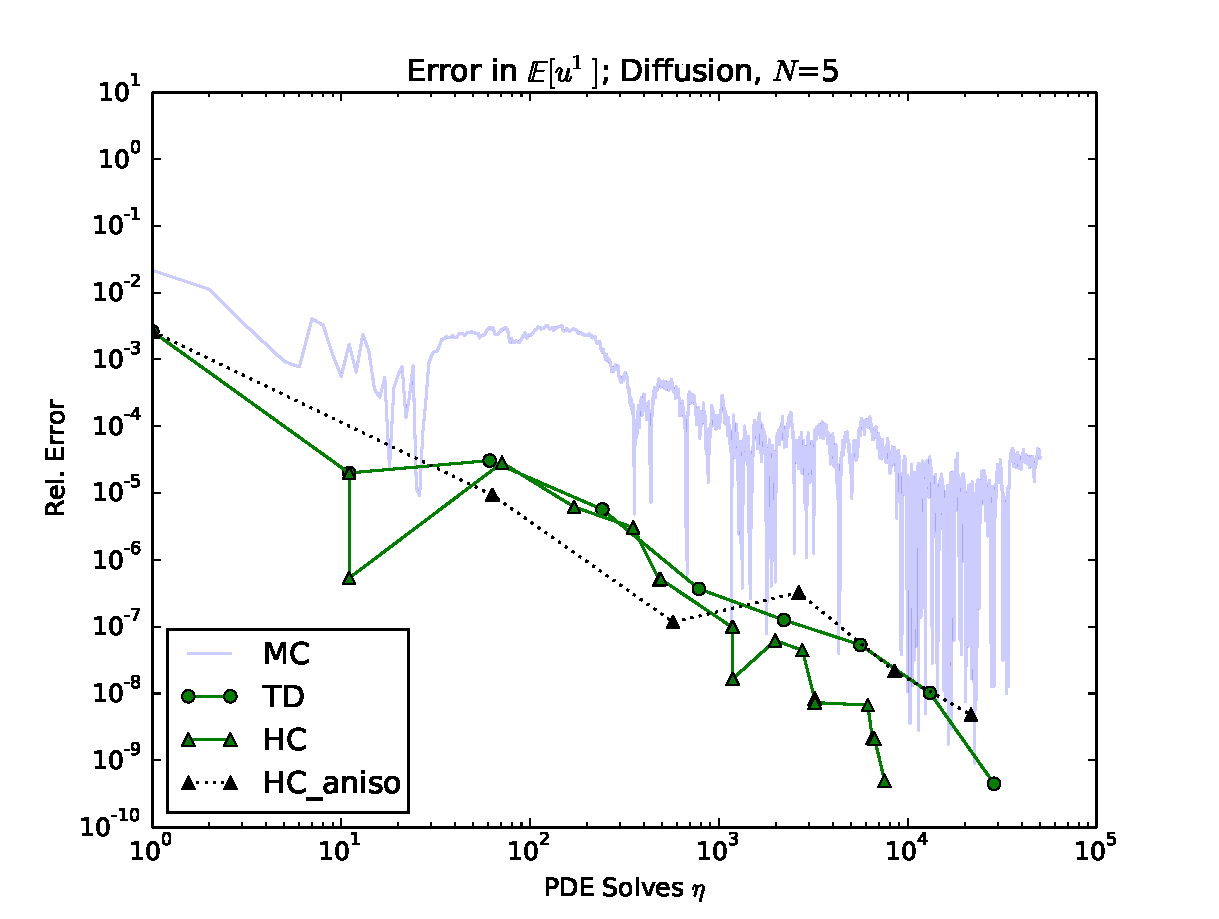
\includegraphics[width=\textwidth]{../graphics/N5_aniso_errs}
      \caption{Error}
      \label{atn errs hdmr}
    \end{subfigure}
  \caption{Diffusion ($N=5$) UQ Results, Mean}
  \label{diff5 anis mean}
  \end{figure}

\begin{figure}[h]
    \centering
    \begin{subfigure}[b]{0.49 \textwidth}
      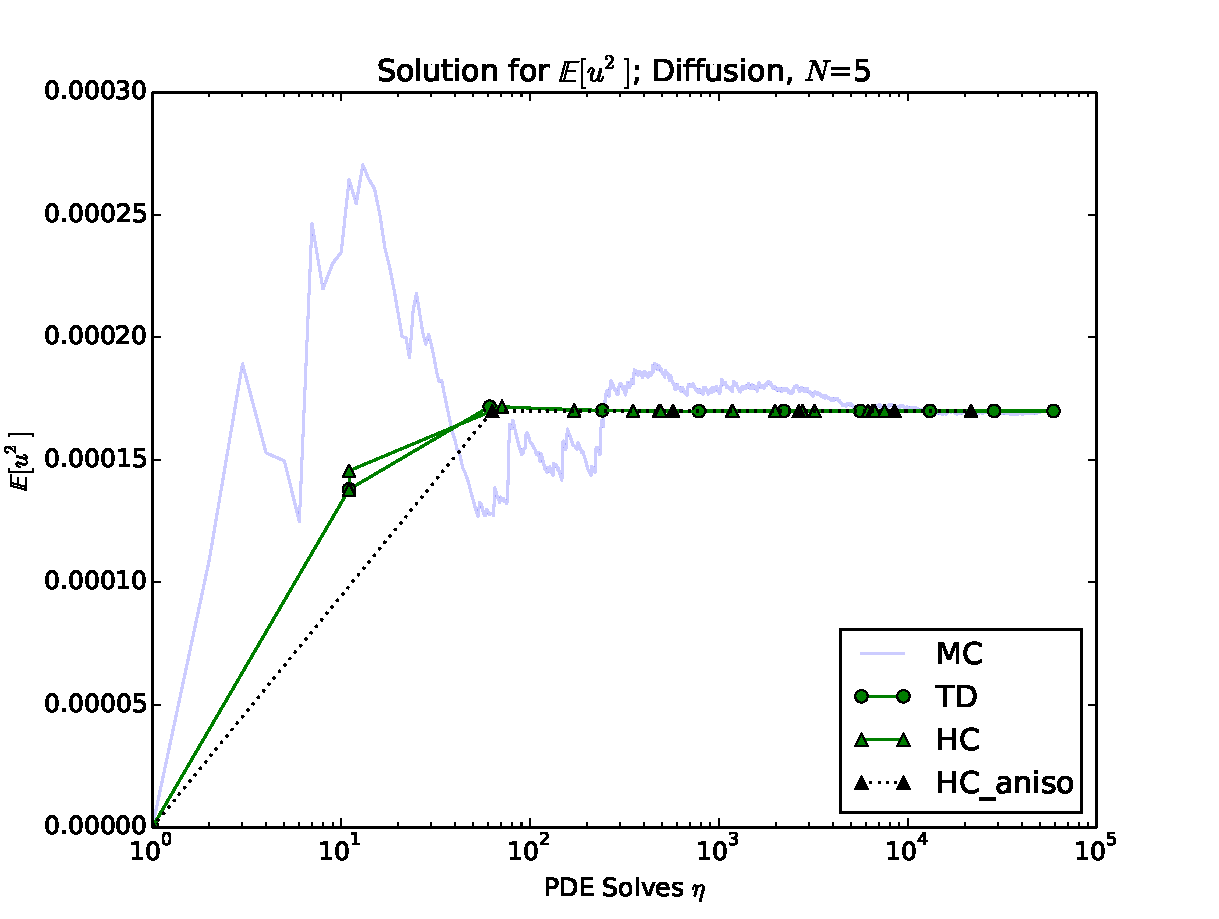
\includegraphics[width=\textwidth]{../graphics/N5_aniso_var_vals}
      \caption{Values}
      \label{atn vals hdmr}
  \end{subfigure}
\begin{subfigure}[b]{0.49 \textwidth}
\centering
      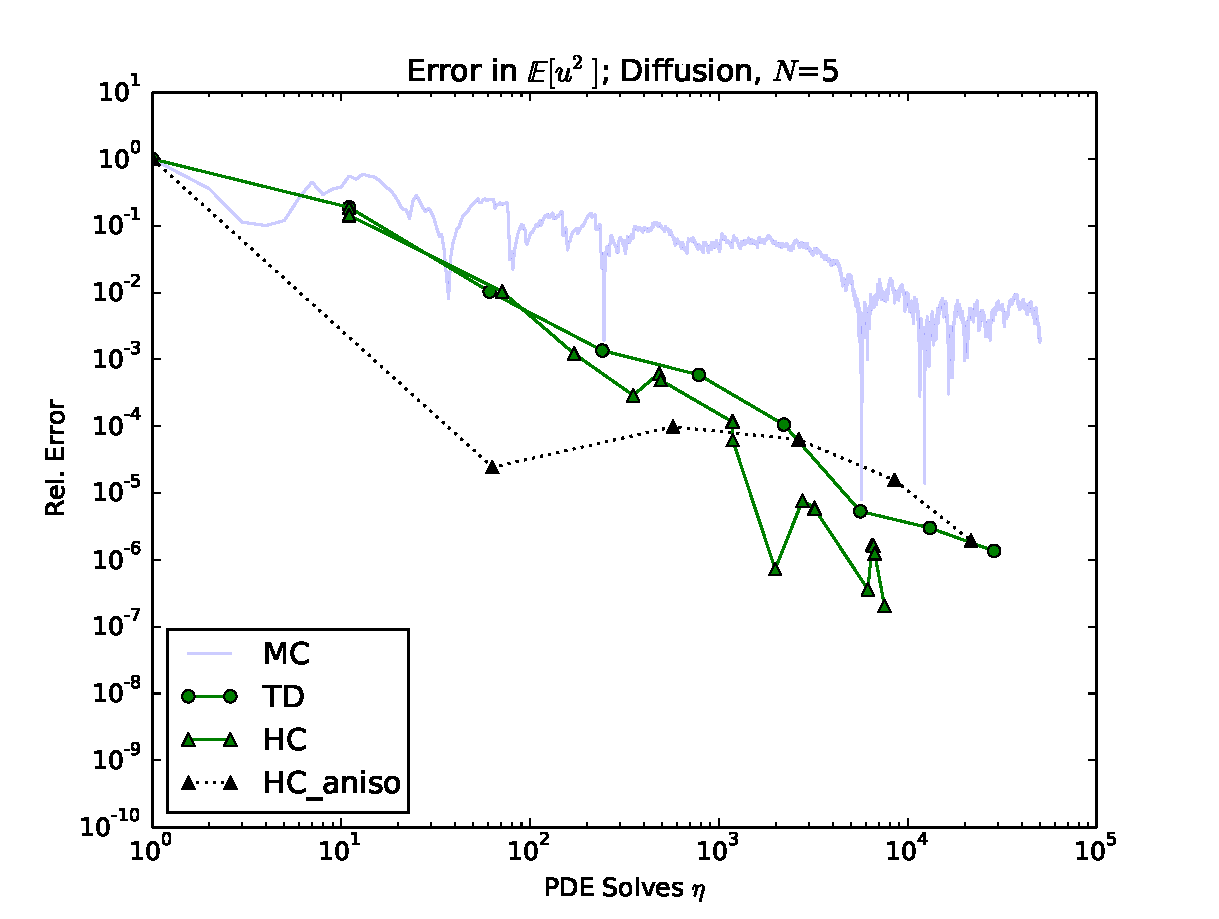
\includegraphics[width=\textwidth]{../graphics/N5_aniso_var_errs}
      \caption{Error}
      \label{atn errs hdmr}
    \end{subfigure}
  \caption{Diffusion ($N=5$) UQ Results, Variance}
  \label{diff5 anis variance}
  \end{figure}


\subsubsection{Diffusion Problem, $N=14$}
Table \ref{tab:diff14 anis} shows values found using an $H_1[u](Y)$ approximation for the projectile problem.  As expected, the capture and fission cross sections in the most prevalent materials have the greatest effect on the $k$-eigenvalue.

As shown in Figures \ref{diff14 anis mean} and \ref{diff14 anis variance}, employing a variance-based anisotropic sparse grid collocation shows some improvement over an isotropic sparse grid.
\begin{table}[h]
\centering
\begin{tabular}{c|c c|c}
$Y_n$ & $Y_n^2$ & $\frac{Y_n^2}{H_1^2[u](Y)}$ & $\alpha_n$ \\ \hline
$D^{(1)}_2$ & 1.75E-13 & 1.8E-13 & 13 \\
$\Sigma_{c,2}^{(1)}$ & 9.86E-6 & 9.9E-6 & 6 \\
$\Sigma_{f,2}^{(1)}$ & 4.80E-6 & 4.8E-6 & 6 \\
$D^{(2)}_2$ & 1.76E-13 & 1.8E-13 & 13 \\
$\Sigma_{c,2}^{(2)}$ & 1.44E-6 & 1.4E-6 & 6 \\
$\Sigma_{f,2}^{(2)}$ & 2.67E-7 & 2.7E-7 & 7 \\
$D^{(3)}_2$ & 2.78E-14 & 2.8E-14 & 14 \\
$\Sigma_{c,2}^{(3)}$ & 6.24E-6 & 6.2E-6 & 6 \\
$\Sigma_{f,2}^{(3)}$ & 2.20E-6 & 2.2E-6 & 6 \\
$D^{(4)}_2$ & 2.12E-14 & 2.1E-14 & 14 \\
$\Sigma_{c,2}^{(4)}$ & 2.05E-9 & 2.1E-9 & 9 \\
$\Sigma_{f,2}^{(4)}$ & 4.59E-10 & 4.6E-10 & 10 \\
$D^{(5)}_2$ & 6.18E-13 & 6.2E-13 & 13 \\
$\Sigma_{c,2}^{(5)}$ & 3.24E-10 & 3.2E-10 & 10
\end{tabular}
\caption{Anisotropies for Projectile Problem}
\label{tab:diff14 anis}
\end{table}
\begin{figure}[h]
    \centering
    \begin{subfigure}[b]{0.49 \textwidth}
      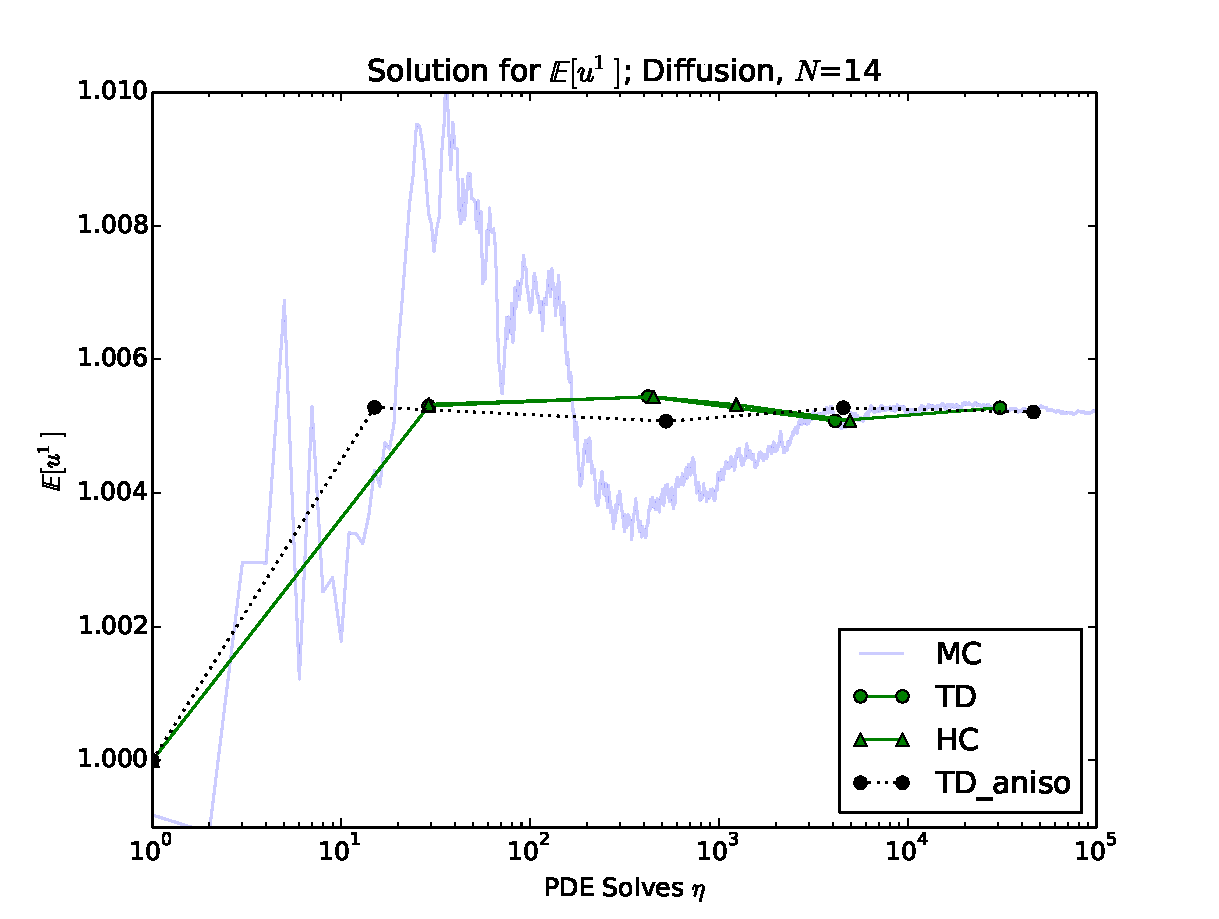
\includegraphics[width=\textwidth]{../graphics/N14_aniso_vals}
      \caption{Values}
      \label{atn vals hdmr}
  \end{subfigure}
\begin{subfigure}[b]{0.49 \textwidth}
\centering
      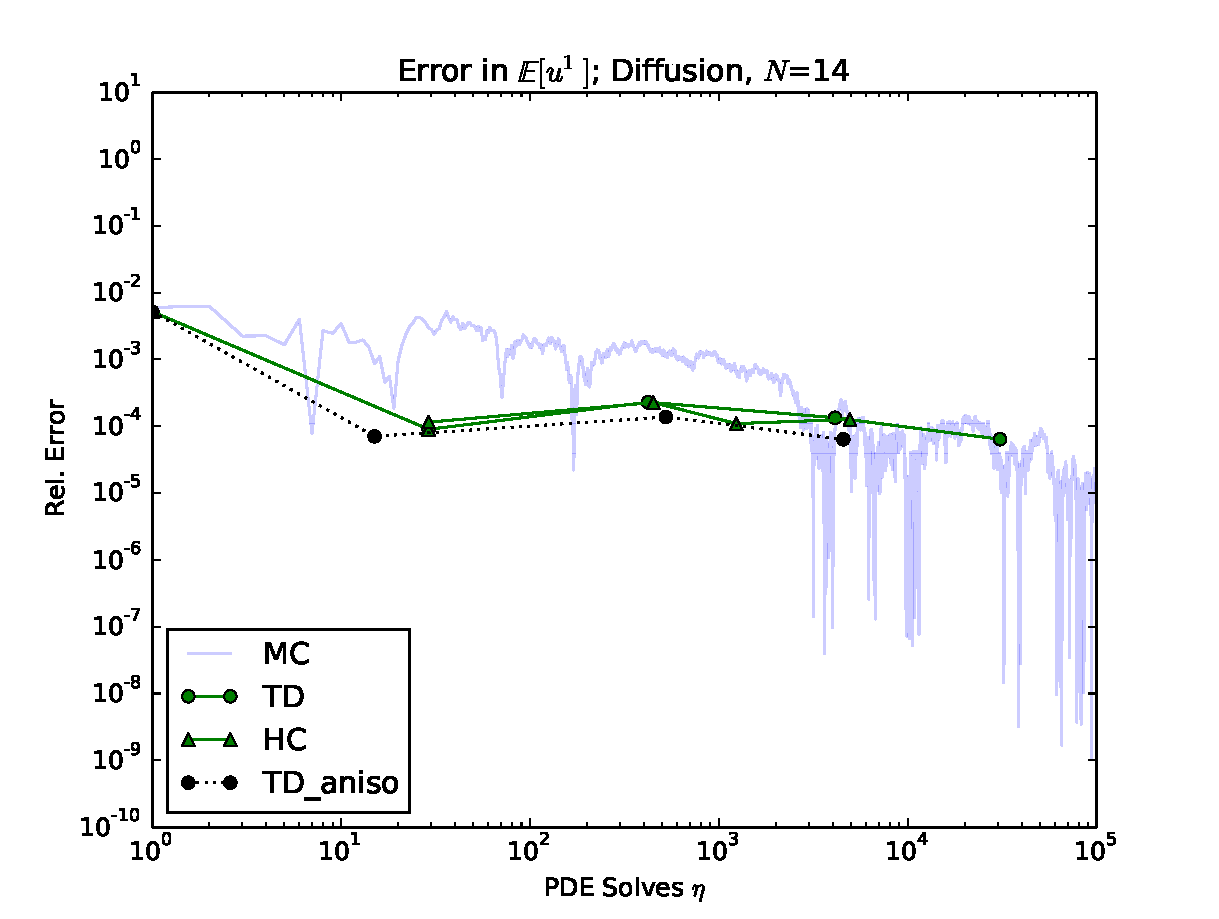
\includegraphics[width=\textwidth]{../graphics/N14_aniso_errs}
      \caption{Error}
      \label{atn errs hdmr}
    \end{subfigure}
  \caption{Diffusion ($N=14$) UQ Results, Mean}
  \label{diff14 anis mean}
  \end{figure}

\begin{figure}[h]
    \centering
    \begin{subfigure}[b]{0.49 \textwidth}
      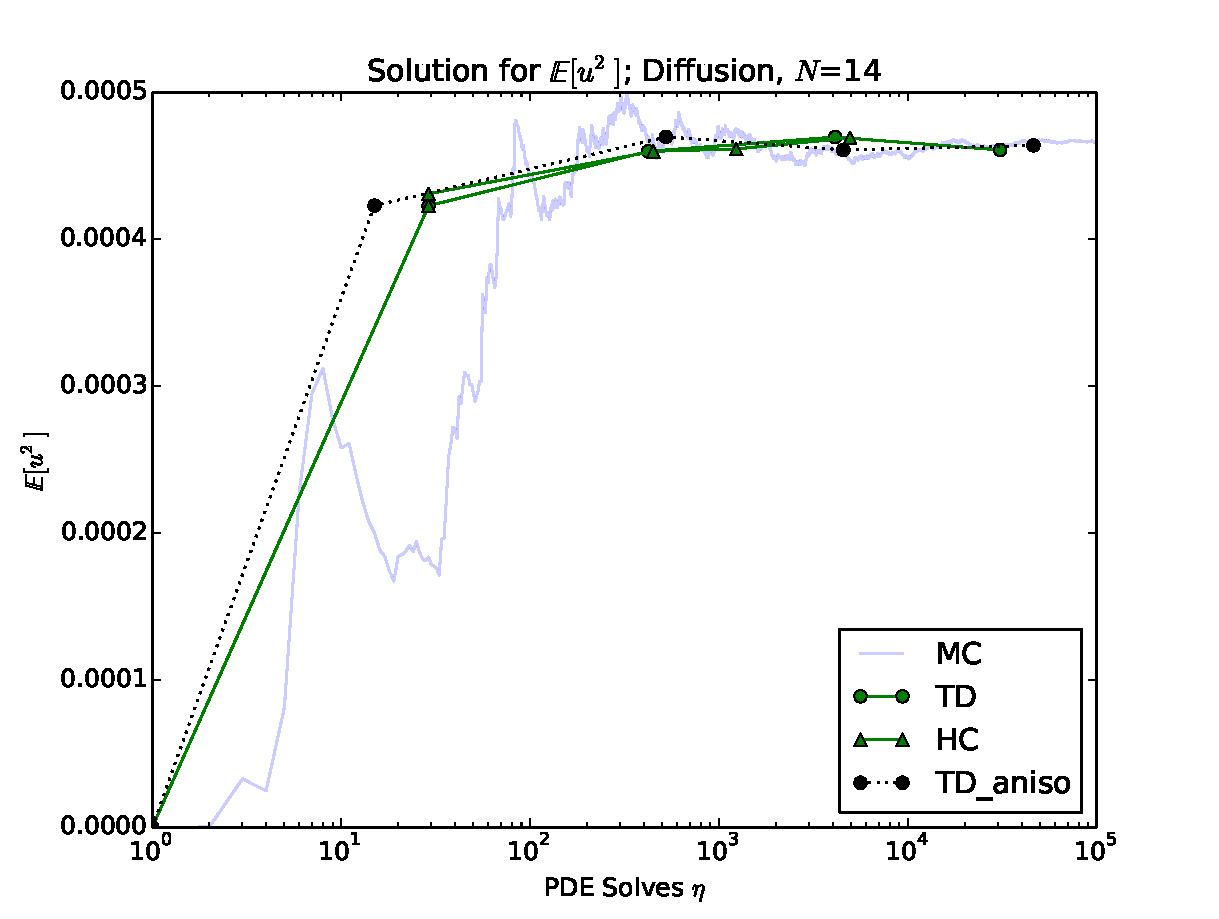
\includegraphics[width=\textwidth]{../graphics/N14_aniso_var_vals}
      \caption{Values}
      \label{atn vals hdmr}
  \end{subfigure}
\begin{subfigure}[b]{0.49 \textwidth}
\centering
      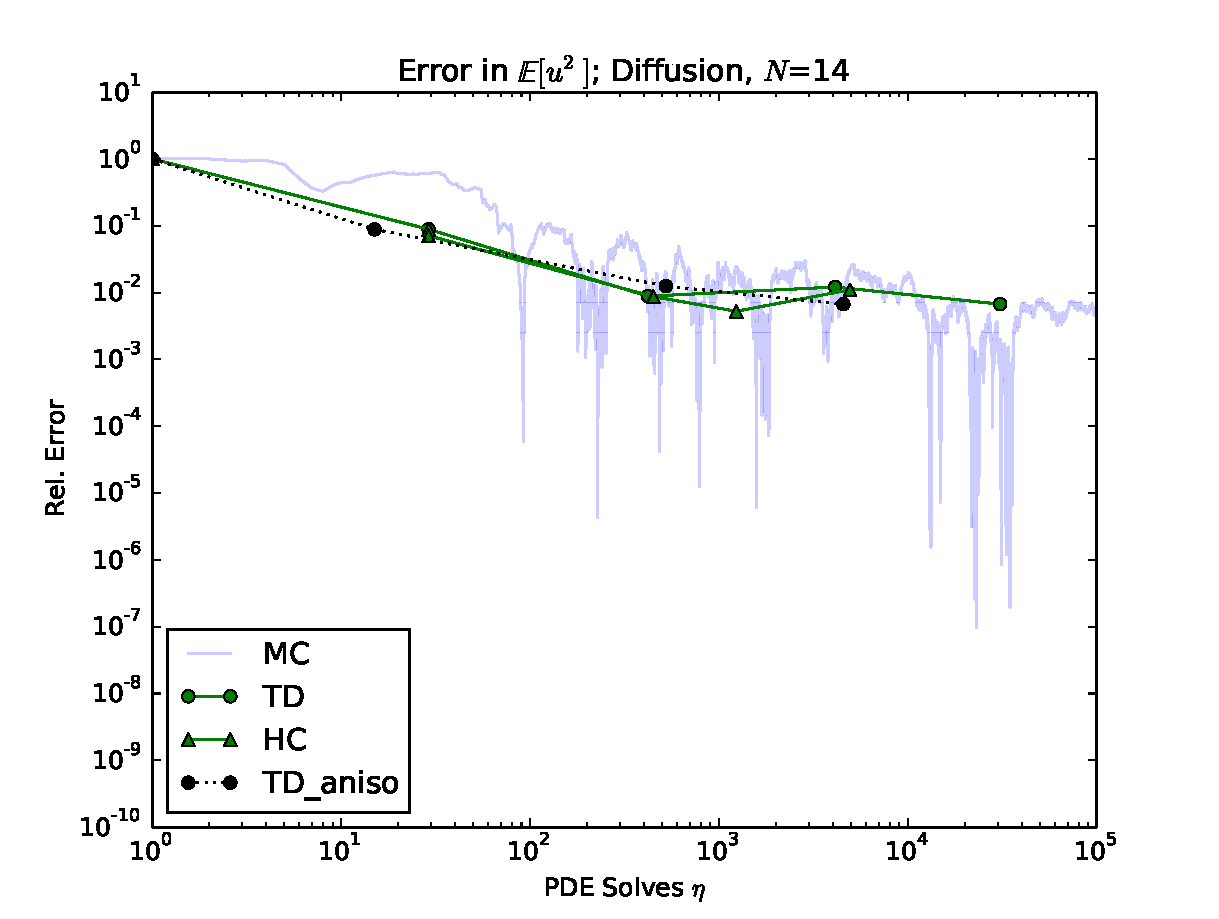
\includegraphics[width=\textwidth]{../graphics/N14_aniso_var_errs}
      \caption{Error}
      \label{atn errs hdmr}
    \end{subfigure}
  \caption{Diffusion ($N=14$) UQ Results, Variance}
  \label{diff14 anis variance}
  \end{figure}


\section{Conclusion}
TODO\\Ongoing:
\begin{itemize}
\item Adaptive Anisotropic Sparse Grid
\item Adaptive HDMR
\end{itemize}
%
%\subsection{Selecting Anisotropy}
%Because of the heuristic nature of anisotropy importance weights, we present here several weight choices and the effect on absolute error and convergence.  We consider four cases along with Monte Carlo and isotropic sparse grids.  Each case is labeled by its importance weights in order of the input parameters listed in Table \ref{params}. The choice of weights is informed by considering the convergence rate of each individual parameter alone with increasing quadrature order, as shown in Fig. \ref{indconv}.  We surmise from this figure that the material 1 cross sections converge the slowest, while the material 5 diffusion coefficient converges most quickly.  We choose the sample cases 1-1-2-2-4 and 1-1-4-4-8 to put increasing weight on the material 1 cross sections and remove weight from the material 5 diffusion coefficient.  In addition, we choose the case 1-1-2-1-1 as an example of a somewhat arbitrary choice of coefficient to remove weight from.  Lastly, we intentionally choose a poor weighting scheme with 8-8-4-4-1 to show worst-case effects of including poor importance weights.  The results are compared in Figs. \ref{aniso1} and \ref{aniso2} for the mean and variance. 
%\begin{figure}[H]
%\centering
%   \includegraphics[width=0.5\textwidth]{coefficient_decay2}
%   \caption{Independent Stochastic Convergence}
%   \label{indconv}
%\end{figure}
%\begin{figure}[H]
%\centering
%  \begin{subfigure}[b]{0.49 \textwidth}
%   \includegraphics[width=\textwidth]{N5_h5_aniso1}
%   \caption{Mean}
%   \label{aniso1}
%  \end{subfigure}
%  \begin{subfigure}[b]{0.49 \textwidth}
%   \includegraphics[width=\textwidth]{N5_h5_aniso2}
%   \caption{Variance}
%   \label{aniso2}
%  \end{subfigure}
%  \caption{$N=5$, Anisotropics}
%  \label{aniso}
%\end{figure}
%
%
%\section{Discussion}
%There are a few important considerations when analyzing Figs. \ref{n1}-\ref{aniso}.\\
%
%First, there is a noticeable plateau in error convergence in many of the stochastic collocation plots.  Thus far this seems to be an artifact of the algorithm, originating in single-point versus double-point precision round off.  Ongoing efforts include finding any conversion of scalars from standard double precision to single precision within the algorithm.\\
%
%Additionally, the number of PDE solves for stochastic collocation is determined based on the maximum expansion level $L$.  For higher $N$, increasing $L$ by only one value increases the number of PDE solves much more than increasing $L$ by one for small $N$.  As a result, there are few data points to power fit for $N=5$, and the plateau just mentioned around $\epsilon=10^{-8}$ is more difficult to distinguish from standard convergence.  Resolving the issues leading to the plateau should also resolve this difficulty in fitting points.  Based on trends with the variance and mean from the other plots, we expect a convergence rate of order -3 for the mean when $N=5$.\\
%
%We can see the possible benefit and harm of applying importance weighting to an anisotropic grid in Figs. \ref{aniso}.  Any application of anisotropic sparse grids in line with our heuristic assessment significantly improves the magnitude of error for a given number of PDE solves.  Even the arbitrarily-chosen 1-1-2-1-1 shows improvements over standard isotropic HC.  We note, however, that the convergence of 1-1-2-2-4 is quite similar to 1-1-4-4-8.  This suggests that with 1-1-2-2-4 we have achieved an optimum efficiency that isn't improved with further anisotropy.  However, the anisotropy intentionally chosen poorly shows much worse convergence than the isotropic case, and for the variance is on par with Monte Carlo.\\
%
%Given these limitations, it is clear that for the uncertain spaces presented, stochastic collocation shows much better convergence and magnitude of error for the same cost when compared with Monte Carlo.  In addition, using judgement to apply an importance weight to variables yields additional rewards in efficiency.
%
%\section{Ongoing Work}
%The work presented here considers a maximum number of uncertain variables $N=5$.  While demonstrative of expected savings for larger input spaces, showing the convergence rates of isotropic and anisotropic sparse grids for large $N$ is desirable.  We expect to see diminishing returns in using stochastic collocation as the input space grows in dimensionality.\\
%
%One effective method for very large numbers of uncertain inputs is HDMR, which uses sets of low-order stochastic interactions between a few variables at a time to approximate the full stochastic problem.  In the event the number of uncertain parameters becomes very large, HDMR could prove less costly than stochastic collocation for many problems. \\
%
%Lastly, our work so far has been demonstrated exclusively with uniformly-distributed random variables as input parameters.  To more accurately approximate the shape of an arbitrary probability distribution, we intend to implement Beta-distributed random variables using Jacobi quadrature, with two shaping parameters $\alpha,\beta$.  The Beta distribution is also distributed finitely between two points, but $\alpha,\beta$ can be adjusted to accommodate a wide range of uncertain distributions including uniform and truncated Gaussian normal distributions.  While Beta distributions cannot exactly replicate all other distributions, we expect it can replicate them without introducing a greater error than introduced by the Monte Carlo and stochastic collocation methods presented.
%
\section{Acknowledgments}
This research was supported by research grants from Idaho National Laboratory.

\setlength{\baselineskip}{12pt}

\bibliographystyle{mc2015}
%\bibliography{references}

%\newpage
\bibliography{../bibliography/uq}
%\bibliographystyle{plain}
\end{document}